\documentclass[pdftex,12pt,a4paper]{report}

\usepackage[pdftex]{graphicx}
\usepackage[ansinew]{inputenc}
\usepackage{geometry}
\usepackage{bbold}
\usepackage{program}
\usepackage[page]{appendix}
\usepackage{subcaption}
\usepackage{url}
\usepackage{textcomp}
\usepackage{gensymb}
% float forces latex to place image right "HERE"
\usepackage{float}
% math utility package
\usepackage{savesym}
\savesymbol{implies}
\savesymbol{overset}
\usepackage{amsmath}
\usepackage{mathtools}
\savesymbol{lneq}
\usepackage{amssymb}
\usepackage[]{algorithm2e}
\usepackage{lscape}
\usepackage{graphicx}
\usepackage{hyperref}
\geometry{a4paper,left=2.5cm,right=2.5cm, top=2.5cm, bottom=3cm}
\newcommand{\HRule}{\rule{\linewidth}{0.5mm}}
\SetKwInOut{Parameter}{Parameters}

% definitions for pseudocode
\newcommand{\forcond}{$i=0$ \KwTo $k - 1$}

% declare macros
%\DeclarePairedDelimiter\ceil{\lceil}{\rceil}
%\DeclarePairedDelimiter\floor{\lfloor}{\rfloor}

% definition for ToC

\usepackage{lipsum}% http://ctan.org/pkg/lipsum
\usepackage{titletoc}% http://ctan.org/pkg/titletoc
\titlecontents*{chapter}% <section-type>
  [0pt]% <left>
  {}% <above-code>
  {\bfseries\chaptername\ \thecontentslabel\quad}% <numbered-entry-format>
  {}% <numberless-entry-format>
  {\bfseries\hfill\contentspage}% <filler-page-format>

\begin{document}
\begin{titlepage}

%%LR
\sffamily

\begin{center}


% Oberer Teil der Titelseite:

\includegraphics[width=0.3\textwidth]{logo2.jpg}
\hfill

\includegraphics[width=0.4\textwidth]{logo1.jpg}  
\\[5cm]

{\Large Department of Mathematics}\\[0.5cm]
{\Large Chair of Mathematical Modeling of Biological Systems}\\[0.5cm]
{Technische Universit\"at M\"unchen}\\[2cm]
{\Large Master's Thesis in Bioinformatics}\\[1.5cm]

% Title
\HRule \\[0.4cm]
{ \huge \bfseries Single-cell analysis of cancer drug response using computer vision and learning algorithms on time-lapse micro-trench data}\\[0.4cm]

\HRule \\[1.5cm]

{\Large Pandu Raharja}\\[2.5cm]

\vfill
\end{center}
\end{titlepage}
%% THIS REMOVES PAGE NUMBER
%%\pagestyle{empty}

%%LR comprehensive title
\begin{titlepage}
{\sffamily


\begin{center}

\includegraphics[width=0.3\textwidth]{logo2.jpg}
\hfill

\includegraphics[width=0.4\textwidth]{logo1.jpg}  
\\[1.5cm]  

{\Large Department of Mathematics}\\[0.5cm]
{\Large Chair of Mathematical Modeling of Biological Systems}\\[0.5cm]
{Technische Universit\"at M\"unchen}\\[1cm]

{\Large Master's Thesis in Bioinformatics}\\[2cm]
{\textbf{\Large Single-cell analysis of cancer drug response using computer vision and learning algorithms on time-lapse micro-trench data}}\\[2cm]
{\textbf{\Large Wirkungsanalyse von Krebsmedikamenten in Einzeller Aufl\"osung durch die Anwendung von Computer-Vision- und Machine-Learning-Algorithmen auf Microtrench- Videoaufnahme}}\\[4cm]

\end{center}
\begin{center}\Large
  \begin{tabular}{ll}
    Author:& Pandu Raharja\\
    Supervisor: &  Prof. Dr. Fabian Theis, Dr. Carsten Marr\\
    Advisor:        &  Prof. Dr. Fabian Theis\\
    & Prof. Dr. Dmitrij Frishman\\
    Submitted:     &  15.12.2017
  \end{tabular}
\end{center}

}% end title page

\end{titlepage}


%%%%%%%%%%%%%%%%%%%%%%%%%%%%%%%%%
% thesis content starts here
%%%%%%%%%%%%%%%%%%%%%%%%%%%%%%%%%

{\parindent 0cm
%%%%%%%%%%%%%%%%%%%%%%%%%%deutsche Version%%%%%%%%%%%%%%%%%%%%%%%%%%%%%%
  
  \section*{Selbst\"andigkeitserkl\"arung}
  Ich erkl\"are hiermit, dass ich die vorliegende Arbeit selbst\"andig verfasst 
  und nur unter Verwendung der angegebenen Quellen und Hilfsmittel angefertigt habe. 
  Weiterhin erkl\"are ich, eine Diplomarbeit in diesem Studiengebiet erstmalig einzureichen.\\
  \vspace{3\baselineskip}
  
  M\"unchen, den \today \hspace{0.1\linewidth}\parbox{0.3\linewidth}{\dotfill}

%%%%%%%%%%%%%%%%%%%%%%%%%%englische Version%%%%%%%%%%%%%%%%%%%%%%%%%%%%%%%%%%%%%%%%%%%%%%%%%%%%%%%%%

\section*{Statement of authorship}
I declare that I completed this thesis on my own and that information which has been 
directly or indirectly taken from other sources has been noted as such. Neither this 
nor a similar work has been presented to an examination committee.

  \vspace{3\baselineskip}
  
  Munich, \today \hspace{0.1\linewidth}\parbox{0.3\linewidth}{\dotfill}
}

\newpage

\chapter*{Acknowledgement}

First and foremost, I would like to thank mom and dad, for the support even from faraway lands. Even though we are continents apart, your pray and hope will be always with me.\\

To Jennifer Carissa, whose support has made it possible to go through the hard parts of my life in the last years. This thesis is only possible because of you.\\

To Julian, Ganesh and other best friends which I resort to for personal assistance. Friends really are hard to find.\\

And finally, to Prof. Fabian Theis, Prof. Joachim R\"adler, Elisavet Chatzopoulou, Felix Buggenthin and Alexandra Murschhauser for tremendous assistant in doing this project. Never did I know a project could be done in this maner.\\

Finally for my best supervisor, Carste Marr. Your boundless patience, deep insight and attention to detail have made this project impossible without your selfless assistance. I hope we could do more things in the future. 

\newpage

\chapter*{Terminology and abbreviations}

{
\flushleft

Following terms are used frequently in this thesis and therefore merit special explanation:

\vspace{10mm}

\begingroup
%\setlength{\tabcolsep}{10pt} % Default value: 6pt
\renewcommand{\arraystretch}{1.5} % Default value: 1
\begin{tabular}{ l l }
\textbf{Name} & \textbf{Explanation} \\
micro-trench & Single unit of micro-trench inside a well \\
wafer & The plate where the micro-trench is manufactured on\\
well & Macro-containment where wafer is located, usually part of larger wells\\
& installation (2 by 4 wells in our case).\\
sticky slide & The containment box where wells are located in\\
slice & An image \\
stack & An ordered sequence of images (usually coming from the same channel) \\
channel & A connection between data source (camera) and storage. Images coming\\
 & from the same channel have same capture properties formatting.
\end{tabular}
\endgroup

\vspace{10mm}

Note that in this thesis, following things are used interchangeably:

\vspace{10mm}

\begin{itemize}
\item image and slice, while referring to an image particularly a capture image of the trenches and its processed versions.
\item image and figure, while referring to an image shown in this paper in general.
\end{itemize}

\vspace{10mm}

\begingroup
%\setlength{\tabcolsep}{10pt} % Default value: 6pt
\renewcommand{\arraystretch}{1.5} % Default value: 1
\begin{tabular}{ l l }
\textbf{Symbol} & \textbf{Explanation} \\
$B_t$ & A 1-bit monochrome image taken at time t (t-th image)\\
$G_t$ & Grayscale image at time $t$\\
$\mathbb{G}_{x, y}$ & Sobel gradient of pixel $M_{t, x, y}$\\
$\mathbb{g}_{x, y}$ & Quadratic Sobel gradient of pixel $M_{t, x, y}$\\
$G(x)$ & One dimensional Gaussian function\\
$G(x, y)$ & Two dimensional Gaussian function\\
$I_t(x, y)$ & Intensity function for pixel $(x, y)$ of RGB image taken at time t $M_t$\\
$I^{conv_G}_t(x, y)$ & Gaussian blurred intensity function for pixel $(x, y)$ of $M_t$\\
$J_t(x, y)$ & Brightness and contrast transforming function for pixel $(x, y)$ of \\
& grayscale image taken at time t\\
$M$ & A stack of images \\
$M_t$ & An RGB image captured at time t \\
$M_{t, x, y}$ & Pixel at $(x, y)$ in $M_t$ \\
$M_{t, x, y, 1}$ & First channel of pixel $M_{t, x, y}$ \\
$M^b_t$ & A $b$-bit encoded RGB image captured at time t\\
$M^m_{t, x, y, i}$ & Pixel-wise mean-substracted pixel $M_{t, x, y}$ \\
$\langle M \rangle$  & Pixel-wise mean image of stack $M$.\\
$T_R$ & Gradient threshold value in a quadtree  (used in RATS algorithm).
\end{tabular}
\endgroup

}
\newpage

\begin{abstract}
Quantitative measurement of cancer drug response is esential to objectively gauge the efficacy of cancer drugs. So far, there has been no method to track and  quantitatively measure single-cell response of of cancer drug treatment. A novel pipeline is presented in this thesis. First, a quasi-high-throughput method to track cells and quantitatively analyze single-cell response to drugs. We investigate the response of model cancer cell lineagues, MOLM and Jurkat, to known anti-cancer drugs Vincristine and Doxorubicine. While the method enabled relatively easy and quasi-high-throughput analysis of cancer treatment \textit{in vitro}, our pipeline could also be adapted in varios contexts involving single-cell analysis with reasonable amount of modifications necessary.
\end{abstract}

\newpage

\tableofcontents

\newpage

\listoffigures

\newpage

\listoftables

\newpage

\chapter{Introduction}

Cancer is among the deadliest diseases ever known to human being. It is a leading cause of death in 2009, second only to cardiovascular diseases \cite{sudhakar2009history}. The numbers are discontenting, especially in the developed world. In the United States alone, half of men and a third of women are expected to develop some kind of cancer. According to US government, in 2016 alone, an estimated 1,685,210 people will be diagnosed with cancer, while 595,690 more will be die from it \cite{cancergov2017stat}.

Worldwide, the International Agency for Research on Cancer's GLOBOCAN series report that, in 2014, \cite{ferlay2015cancer}.

\begin{verbatim}
I.
- readable to people without background in the fields
- non technical at all
II.
- what have the researches done
-- biologics
-- technicals
III.
thesis overview
4~8 pages
\end{verbatim}

%TODO organize this part

Generally, following questions are to be investigated in the experiment:

\begin{itemize}
\item We would like to investigate the dynamics of the AML-M5a MOLM-13 cell line's response towards chemotherapeutic treatment regimes in various drugs' concentration levels (for both Vincristine and Daunorubicin).
\item We also would like to look into the effect of cell cycle on the the AML-M5a MOLM-13 cell line's response to drugs. Specifically, following questions needs to be answered: does the response of cancer cells depends on cell cycle?
\end{itemize}

To answer aforementioned questions, we designed the experiments as follow.

\section{Variability of cell-to-cell response towards cancer treatment}

%TODO : modify to local use

Cell-to-cell variability in response to external stimuli is a pervasive trait in cellular systems that prevails even in isogenic cell populations. Here, heterogeneity might be caused by epigenetic modifications, differences in the cell cycle phase, or by intrinsic stochastic fluctuations in gene expression and biochemical regulation. The implications of heterogeneity for cancer progression and treatment are poorly understood. In some cases, heterogeneity is dominated by intrinsic fluctuations in the stochastic expression of key regulators that randomly alter the sensitiveness of individual cancer cells. A raw model of this scenario has been put forward in recent work on TRAIL-induced apoptosis [1, 2]. Experiments and simulations show that variability in cell fate is sensitive to small stochastic increases in the levels of Bcl-2 and are transiently heritable to siblings [3, 4]. The study on TRAIL-induced apoptosis led to a novel interpretation of fractional killing and predicts reversible resistance to chemotherapy. The profound consequences for cancer treatment have been subject to theoretical studies on the stochastic origins of cell-to-cell variability in cancer cell death decisions [5-7]. 
Cancer is an intrinsically highly diverse disease; tumors of any different histological type not only exhibit genetic diversity but also display their variation when exposed to all forms of chemotherapy [8]. Most state of the art chemotherapeutic drugs in clinical use, target rapidly dividing cells and trigger apoptosis. Vincristine (VCR), an antitumor vinca alkaloid, binds to tubulin and stops the dividing cell from separating its chromosomes during metaphase in M-phase. It is thus considered an M-phase dependent drug [9]. In contrast, daunorubicin, an anthracycline aminoglycoside antineoplastic, intercalates on DNA and inhibits the function of the enzyme topoisomerase II during transcription and replication. Daunorubicin is thus expected to act throughout the whole cell cycle and but especially strong during the DNA replication in the S-phase. Both drugs are used to fight hematopoietic disorders such as Acute Myeloid Leukemia (AML)[10, 11] among other neoplams. In the literature, a drug that interferes with the cell cycle is in general considered cell cycle dependent, but in practice it is not clear whether it only acts on a specific cell cycle phase, due to side effect toxicities. Based on this, it is hypothesized that both VCR and daunorubicin are cell cycle dependent. Since it is assumed that VCR acts only during M-phase in their cycling, we can expect that cells that are closer to M-phase will die earlier [12, 13].  
It is essential toTo understand sources of heterogeneous response of to cancer in therapy and , in order to design novel therapeutic strategies and potent agents,  that not only targets key signaling pathways with high specificity but also address the contextual role of cell cycle timing in cancer therapyin the response of cells to chemotherapeutic drugs has to be investigated. In this context, time-lapse imaging, which allows for recording accurate histories of individual cancer cell fates and cancer subpopulations, received increasing attention [12, 14, 15]. However, the to study the effect of particular cell cycle phases on chemo sensitiveness, single cells have to be observed continuously throughout division, drug addition, and death.  has not been explored at the single cell level. 
The typical bottleneck for a high-throughput analysis for such is cell tracking. Tracking single cells in time-lapse microscopy movies is a challenging problem. Different automatic image analysis tracking tools have been proposed [19,20 ] and compared [16,17]  [16-20]  but to achieve tracks for for fast moving cells movements, high cell densities, challenging cell identification, and long-term observations, also time-intensive manual tracking becomes necessary to achieve accurate tracksis often applied [18,21] to generate tracks with maximal accuracy. For many approaches, the workload of manual tracking has to be compared to correcting erroneous track from tracking algorithms [schröder review].   [21] . Confining cells spatially obviously reduces possible tracking errors and facilitates the application of tracking algorithms. In particular, non-adherent cells are painstaking to track since diffusive and convective drift in long-term measurements complicate cell assignments [20]. Among the techniques to capture non-adherent cells for long-term observation microfluidic devices [22] as well as micro-well platforms [23-28] were have been developed. Alternatively, individual cell cycle phases were imaged using fluorescent cell cycle reporters [29].  The confinement of single cells into well-defined spatial structures provides a straightforward implementation to facilitate automatic tracking since long-term crossing of individual tracks is avoided. PConsequently, platforms that confine single starting cells and thus lead to spatially separated cell families (also called clones) are an especially derived from a single mother cell are a useful tool to investigate cell cycle length, sister cell correlations, or the effect of cell cycle phases to to enable the automatization of the image analysis and to yield in a faster and effortless way to collect time traces that can address questions regarding the sources of cell-to-cell variability in a high-throughput manner. 
Here we introduce a platform that enables the continuous observation of cell families derived from individual non-adherent cells of the leukemia cell line MOLM-13. The platform employs arrays of micro-trenches optimized to observe cells for two consecutive generations. We demonstrate that automated image analysis is feasible and allows for precisely determination determiningof the cell division cycle time  distribution and sister cell correlations. A key feature of the platform is the direct and parallel observation of many hundreds of cells with individualin different cell cycle statess. We show that the time-to-death after induction of apoptosis of the leukemia cell line MOLM-13 using the anti-mitotic agent vincristine (VCR) and daunorubicin (dauno) has a small dependence on cell cycle . The results were found consistent with experiments using cells that were synchronized using standard thymidine cell cycle arrest. Using arrays of micro-trenchesOur approach also enabled a time correlation analysis which showed that the time-to-death of daughter cells correlates with the time spent in cell cycle, while this effect is not detectable when cells are synchronized. 


\section{Hypothesis}

In this part, the hypothesis underlying the experiment is presented.

\section{Advances in microfluidics, image processing and machine learning}

In the recent decades, as in many other fields, there are numerous groundbreaking advances in the fields of microfluidics, image processing and machine learning.

%TODO : continue

The advances, coupled with general technological advances in computing power and energy efficiency, have made it possible for us to design almost completely automated analytical pipeline for single-cell microfluidic system.

%TODO : expand

While not all methods and algorithms in this project are the most recent, many of them are state-of-the-art and/or good enough for the pipeline to work seamlessly.

\subsection{Microfluidics}

As the name suggests, 'microfluidics' concerns the manipulation of fluids in a small working dimension, typically starting from nanometers to lower millimeters \cite{whitesides2006origins}. In modern context, the entire fields tries to find application of micro-sized devices which hold and control the state of liquid \cite{whitesides2006origins} including cell culture medium. There are two categories of microfluidics: active and passive microfluidics devices. The separation is based on the device's ability to actively manipulate the flow and control of devices \cite{sekhavati2015dynamic}. Active devices use micro-valves to perform sophisticated chemical processes \cite{marsden1993interdisciplinary}. This goes as far as reactions at individual cell level \cite{eyer2012microchamber}. A passive device, which our micro-array system is, exploits on the other hand its physical property to provide rapid controlled environment for micro-sized experiments.

Active microfluidic methods for analysis and manipulation of biological cells have been done in various way and form. In 2003, Wheeler \textit{et al} developed a novel microfluidic device from poly-dimethylsioxane using multilayer soft lithography technology for the analysis of single cells \cite{wheeler2003microfluidic}. The microfluidic setup facilitates the passive and gentle separation of a single cell from the bulk cell suspension. This in turn enables the precise delivery of reagents as little as one nanoliter to the cell. In other use cases, the optical-based microfluidic methods have been used to sort cell with very high accuracy \cite{macdonald2003microfluidic}. This family of method utilizes the fact that different dielectric particles respond differently to an applied light field \cite{tatarkova2003brownian}. Combined with the miniscule spatial setting, the methods are compatible for single-cell resolution analysis. For example, optical-based microfluidic methods have been used to sort cells with very high accuracy \cite{macdonald2003microfluidic, wang2005microfluidic, baret2009fluorescence}.

As a method, passive mocrofluidic methods are mostly used to provide specialized environment in cell-size resoultion. For example, microfluidic settings have been used to keep spatio-temporal identity of single cell for the analysis of the underlying biological dynamics of the isolated cells \cite{mu2013microfluidics, sekhavati2015marker}, which form the methods the design and synthesis of our micro-trench system are based on.

In the last decades, the recent advances in both passive and active microfluidics have created an entire field \cite{whitesides2006origins} with use cases ranging from \textit{in vivo} imaging \cite{chronis2007microfluidics}, single-cell analysis \cite{wheeler2003microfluidic} to cellular biophysics \cite{di2010bacterial}. This project leverages in these advances coupled with equally outstanding advances in image acquisition, image processing and machine learning methods which will be described in the subsequent subsections.

The use of microfluidics enables us firstly to study the distribution of division times among single cells and also to correlate the division times between sister cells, which are genetically very similar. Secondly, the array of micro-trenches enabled the study of the response dynamics of single-cells to doxorubicin, a widely used chemotherapeutic drug, and the comparison of the response to this agent between a chemically synchronized and a non-synchronized population

\subsection{Image Processing and Computer Vision}

\label{subsection:cv_advances}

Before the runaway advance of deep learning methods in the last years, object and area detection methods generaly rely on disciminating certain patterns and features in the picturek -- with and without utilizing machine learning methods. In 2001, Paul Viola and Michael Jones proposed a method that was able to recognize face \cite{viola2004robust}, and later, objects in almost real-time fasion \cite{viola2001rapid}. %TODO continue with viola jones

%TODO fill

\subsection{Machine Learning}

\label{subsection:ml_advances}

%TODO fill

\section{Comparison with other methods}

\subsection{Cell death determination}
\label{subsection:comp_cell_death_determination}

%TODO modify

Measuring cell death is a crucial part of the experiment, as the reliable determination of it is the basis of most analysis in this thesis. There are several way to measure cell deaths with varying complexity and accuracy. Each method contains certain assumptions of cell death.\\

For example, determining cell death by cell movement assumes death of a cell if no movement beyond random flux is observed in certain amount of time. This obviously has certain drawbacks, such as when the observation is done in non-static environment. Moreover, defining the limit of the random flux, above which a given cell is assumed to actively move, is not a trivial task. Some kind of gold standard for a given cell line and environment has to be established manualy, which is very time consuming. This fact is again made even more complicated by the fact that many cells show different movement pattern upon introduction of treatment. It is well known that some cells tend to move faster or slower under stress, the situation many cancerous cells in our experiment will experience upon addition of cancer drug treatment \cite{pienta1991effects, fenteany2003small, ruocco2012suppressing}.\\

The second method is using cell size. During apopotosis, the cells would shrink. Given It is known that cell size %TODO continue.

\subsection{Other model cell lines}

%TODO modify


Some other cell lines were examined as potential probe cell line in this experiment. One of them is Jurkat Cell, a model cell commonly used to study T Cell Leukimia, T cell signalling mechanism and the expression of various HIV-related chemokines \cite{schneider1977characterization}. The cell line was a considered since it is well-studied \cite{johnson2007genome, schena1996parallel}. This is especially true if we consider apoptotic mechanism of the cell line, a problem this project and other related projects by our  and partner labs are trying to investigate. There are several seminal publications about the dynamics of apoptotic mechanism of Jurkat cells we could well compare our results to \cite{gottlieb1996apoptosis}. Samali \textit{et al} \cite{samali1999presence} even studies the dynamics of Caspase expression in Jurkat cells, a topic dealt a lot in this project as the chapters progress (see for example Subsection \ref{subsection:treatment}) while Kasai \textit{et al} considers the aspect of spindle checkpoint in the context of apopototic cell death \cite{kasai2002prevalent}. However, we figured out early on that the cell motility of the Jurkat cell line was increased dramatically (a phenomenon observed by others before us \cite{barnhart2004cd95}) upon the introduction of chemotherapeutic treatment -- the increase dramatic enough that the cells managed to escape the micro-trench it initially landed in.

\section{The structure of the thesis}

%TODO fill

The thesis is presented as two closely-related things. First, we present high throughput system that enables analysis in single-cell resolution of cells' response towards certain chemical reaction and a software suite that processes, analyzes and visualizes the data. This is an end-to-end solution that possibly can help researcher in their research. Second, we apply this method on the main question of the project: the response dynamics of cancer cell towards chemotherapeutic treatment. Here several questions are posed and addressed using the system and software suit.

%TODO improve

%TODO add chapter one

Chapter \ref{chapter:data_and_method} contains %TODO continue

\chapter{Data and Methods}

\label{chapter:data_and_method}

As mentioned in previous parts of this thesis: this project consists of three part -- the problem statement regarding the dynamics of cancerous single-cells under pressure of treatment, the microfluidics which enables the single-cell protocol and the software implementation used to process and analyze the time-lapse data coming out of the experiment.

This chapter considers two aspects of the project: the experimental setting and the theoretical aspects behind the data analysis pipeline. In the first half of the chapter, we deal mostly with the experimental background and the underlying questions of single cell dynamics of cancer cell under stress with focus on chemotherapeutic pressure. In this part, the highlight of the experiment, the microfluidic system for cell containment is elucidated. In conjunction with the system, some biomedical and biochemical aspects of the experiment are also mentioned. This includes the drug, the auxiliary chemicals used in the experiment and the cell lines probed. The second part deals mostly with the quantitative methods and algorithms used to process data into meaningful observations. This part is opened with definitions used in the methods section.

\section{Experimental setting and data}

\subsection{Cell culture}
\label{subsection:cell_culture}

To enable cross reference and comparability of experiment results, a model cell line is used: the acute monocytic leukimia (AML) cell line \textbf{AML-M5a MOLM-13}. The line used in our experiment was derived from the cell line initially described by Matsuo et al in 1997 \cite{matsuo1997two}. In the paper, the authors developed the line from the peripheral blood of a relapse patient with AML of subtype FAB M5a, which is characterized by predominantly monoblastic leukemia cells visible in pap smear \cite{arber20162016}. Due to extensive research done on the cell line and the well-explained mechanism of the cell line dynamics and response towards cancer medications, the cell line is an ideal candidate for \textit{in vitro} study of monocytic differentiation, leukemogenesis and treatment dynamics \cite{matsuo1997two, kelly2002ct53518, yokota1997internal}.

For our experiment, the AML-M5a MOLM-13 cell line was cultured in Gibco\textsuperscript{\textregistered} RPMI 1640 GlutaMAX medium, produced by Life Technologies \cite{gibcocellculture2017}. The medium is popular choice in human cell biology for both experiments and biological syntheses using human cells and their derivatives \cite{blight2000efficient, shimizu2002fabrication}. It is pre-supplemented with stable form of L-glutamine to prevent ammonia buildup, a common and serious problem in cell culture due to its cell toxicity\cite{satter1974effect}. The medium is further supplemented with Gibco\textsuperscript{\textregistered} Fetal Bovine Serum (FBS), also offered by Life Technologies \cite{gibcofbs2017}, as supplement for the AML-M5a MOLM-13 cell culture.


\subsection{Microfluidics}
\label{subsection:microfluid_env}

In our cases, the microfluidics is designed by the Soft Condensed Matter Group at the  Faculty of Physics at the Ludwig-Maximillians-Universit\"at M\"unchen. There are several papers related to the system. For example, in 2013, Marel et al proposed the method of creating micro-wells for single-cell containement based on three-dimensional poly(ethylene glycol)-dimethacrylate (PEG-DMA) microstructures \cite{marel2013arraying}. Later on in 2015, Sekhavati et al publishes the first design of micro-trench arrays that are used in our experiment \cite{sekhavati2015marker, sekhavati2015dynamic}.

In order to track non-adherent cells in a label-free manner over several generations, a set of micro-trenches ($30 \times 120 \, \mu m$) out of PEG-DA (Polyethylene(glycol) Diacrylate), which can accommodate four to six cells are designed and fabricated. The platform facilitates cell tracking leading to the observation of hundreds of families of cells, derived from one single mother at each case.

First, the SU-8 (MicroChem Corp, USA) wafer was fabricated in a cleanroom facility using a ProtoLaser LDI system (LPKF Laser \& Electronika, Naklo, Slovenia), with a 375 nm wavelength laser and 1 μm spot diameter.
Polydimethylsiloxane (PDMS) prepolymer solution is mixed with the crosslinker in a 10:1 ratio (w/w) (Sylgard 184, Dow Corning, USA) and then degassed under vacuum. PDMS is then purred on the SU-8 wafer, degassed and cured in 50 \degree C. The resulting PDMS stamp is peeled off the wafer and cut into appropriate shapes. The PDMS pieces, with 25 1/4 pillars in height, are activated with argon plasma and then immediately placed upside down on a silanized with TMSPMA (3-(Trimethoxysilyl)propyl methacrylate, Sigma-Aldrich) glass coverslip. A solution of PEG-DA (Mn=258) containing 2\% v/v of the 2-hydroxy-2methylpropiophenone (both from Sigma-Aldrich, Germany) is freshly prepared and then a drop is deposited at the edge of the PDMS stamp. The PDMS stamp is filled by capillary force induced flow. PEG-DA is then polymerized in an UV-ozone cleaning system (UVOH 150 LAB, FHR, Ottendorf, Germany). Next, the PDMS stamps are peeled off and the resulting micro-trenches of cross-linked PEG-DA are dried in an oven (Binder GmbH, Tuttlingen, Germany) overnight at 50 \degree C. Finally, the slides are sonicated with 70\% ethanol and distilled water before a sticky slide is attached on top (8-well sticky slide, ibidi GmbH, Munich, Germany).

The design of the micro-trench and the schematic representative of cell tracking are seen in Figure \ref{fig:microtrench_design}. After the manufacturing process the structure is divided into two main parts:

\begin{itemize}
\item The micro-trenches are The smallest structure of the setting, measuring about 120 microns by 30 microns. The base of the trench is made of Polyethylene (glycol) Diacrylate (PEGDA), an inert substance commonly found as construction material in microfluidic system \cite{sekhavati2015marker}. Each well contains about 2400 micro-trenches contained in one containment box.

\item The sticky slide contain 8 wells where the wafer containing micro-trenches is located. The sticky slide chosen for containing the wafers holding the micro-trenches is ibidi\textsuperscript{\textregistered} sticky-Slide 8 Well (see Figure \ref{fig:ibidi}). In the project, each cell treatment is isolated in one containment box. This ensure the separations of different chemicals used in each treatment.

\end{itemize}

Due to limitations in the image capturing coverage area, each well is further divided into eight image positions. Each image position represents an area the camera captures the full image of. In each well there are 7 to 8 image positions and in one experiment with eight wells there are 63 image positions in total. Tables  \ref{table:unsyn_treatments} and \ref{table:syn_treatments} show the list of all image positions in the experiment and their drugs concentration.

\begin{figure}[H]
\centering
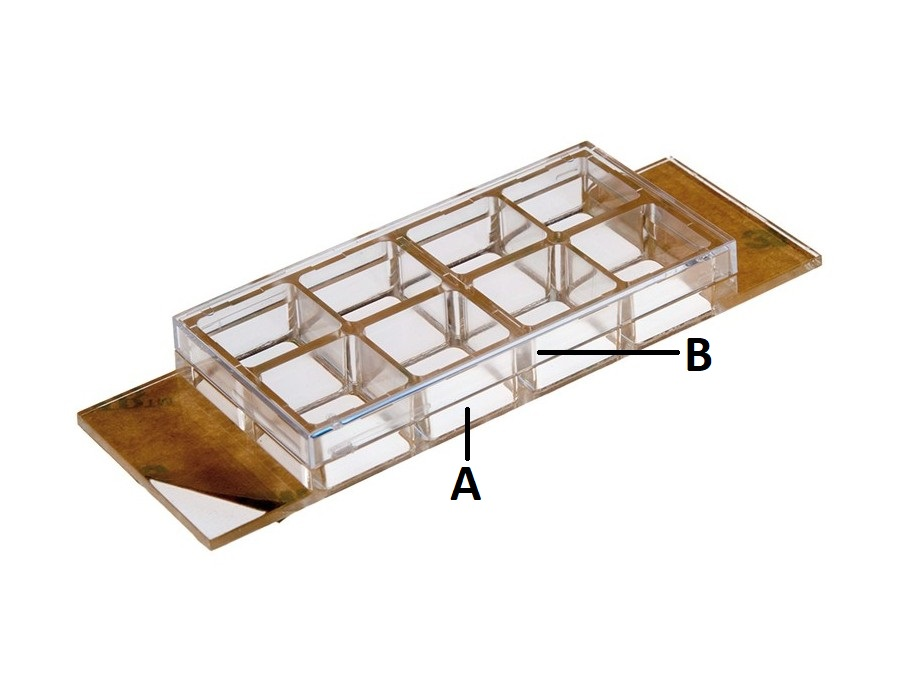
\includegraphics[width=\textwidth]{images/sticky-slide-8-well-marked}
\caption[ibidi\textsuperscript{\textregistered} sticky-Slide 8 Well]{ibidi\textsuperscript{\textregistered} sticky-Slide 8 Well. The base SU-8 wafer is located in each of the containment box \textbf{(A)}: the SU-8 wafer is then fabricated in the surface of each containment box using nano photolitographic printing. The microfluidic system is then poured and stamped on top of the wafer. Note that each containment box is upside-open. \textbf{(B)}: the cap is used to prevent the ingress of foreign materials into the medium. \textit{Image taken and modified from ibidi GmbH's website}.}
\label{fig:ibidi}
\end{figure}

\begin{figure}[H]
\centering
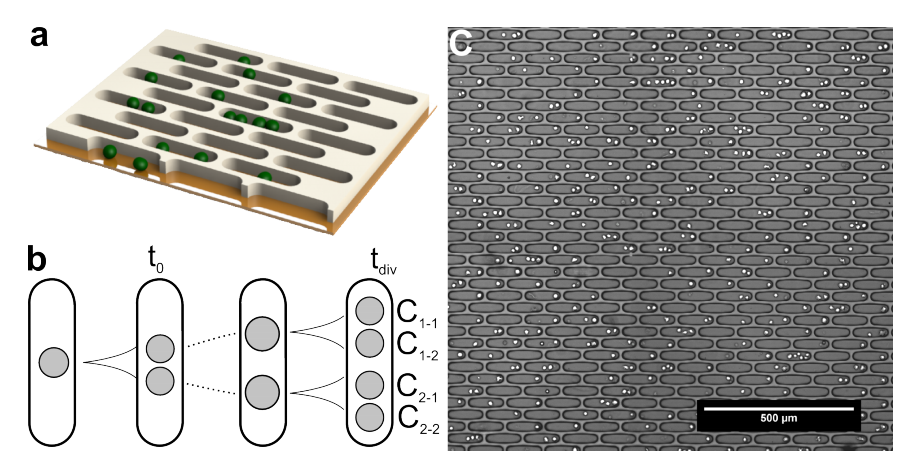
\includegraphics[width=.9\textwidth]{images/trenches-sekhavati}
\caption[The structure of micro-trenches]{The structure of micro-trenches: \textbf{(A)} 3D model of micro-trench on surface with cells inside. \textbf{(B)} The schematic representation of a time-lapse in a trench. First, a singly-placed cell is tracked in a micro-trench. At time $t_0$, the cell divides into two daughter cells. The two cells will be kept tracked until at one point each of the daughter cells will divide at the same time at time $t_{div}$. Note the simplification of the sample. First, not every cell is singly-placed inside a trench. Indeed, not every trench is occupied by cells. Second, not every cell divides. Third, not every cell line observed has three generations in it. And finally, not every children's division times are at the same time. Indeed, this special case almost never happens in real life. \textbf{(C)} The sample view into the environment with cells occupying some micro-trenches. Here, the micro-trenches have dimension of 120 $\mu m$ long and 30 $\mu m$ wide. Note also the pointish characteristic of the cells taken in out-of-focus fashion. This improves the performance of the tracking algorithms. \textit{Figure taken from (Sekhavati, 2015) \cite{sekhavati2015dynamic}}.}
\label{fig:microtrench_design}
\end{figure}

\begin{figure}[H]
\centering
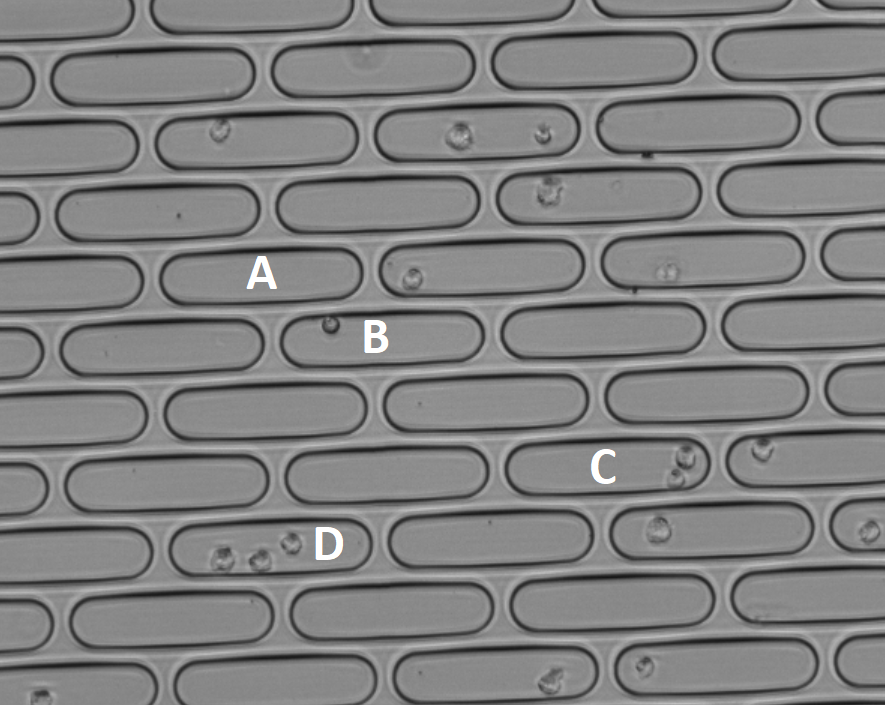
\includegraphics[width=0.55\textwidth]{images/microtrench_in}
\caption[The typical view of micro-trench setting]{The typical view of micro-trench setting. Some trenches contain no cell at all \textbf{(A)}. Several trenches contain exactly one cell \textbf{(B)}. A few more trenches contain two cells \textbf{(C)} while in rare cases the trench may contain more than two cells \textbf{(D)}.}
\label{fig:microtrench_sample}
\end{figure}

\subsection{Cancer treatment regimes}
\label{subsection:treatment}

As mentioned in previous chapters, the objective of the project partains mostly the dynamics of single cancer cell under treatment. After mentioning the cell lines of interest (Chapter \ref{subsection:cell_culture}) and the microfluidic setup used to contain cancer cells in single-cell setting (Chapter \ref{subsection:microfluid_env}), we arrived at the last aspect of the experimental seting: the chemical treatment used on the cells.

For cell cultures mentioned in the previous subsection, two drug treatment regimes are developed: Vincristine and Daunorubicin -- both chemotherapeutic compounds well known for treating various kinds of cancer \cite{drugs2018defdaunorubicin, ravina2011evolution, tsuruo1981overcoming, gewirtz1999critical}.

\subsubsection*{Vincristine}

Vincristine, a vinca alcaloid, is initially isolated from the Madagascar pairwinkle \textit{Catharanthus roseus} (basionym \textit{Vinca roseus}, hence the name) \cite{nci2018defvincristine}. It is mainly known as Tubulin polymerase inhibitor \cite{tsuruo1982increased}, a subclass of the mitotic inhibitor family of drugs \cite{jordan1998tubulin}. Mechanistically, it prevents Tubulin polymerization in two ways. First, it binds elongating Tubulin polymer and reduces the affinity of the elongating polymer \cite{lobert1996interaction} towards Tubulin monomers threfore preventing the monomers to bind on the elongating polymer. Meanwhile, further elongation by the polymers is also prevented via allosteric inhibition. It has also been shown that Vincristine depolymerizes stable microtubuli in the axonal part of rats' neuron cells \cite{jordan1998tubulin}. Due to these mechanistic actions, the effect of Vincristine is most emphasized during the time of high Tubulin synthesis, e.g. during the separation of chromosomes in the Metaphase by means of tearing them with the simultaneous pulling and pushing mechanism of Tubulin poly- and depolymerization \cite{owellen1972binding}. In the context of chemotherapy, Vincristine is often used as combination in CHOP (cyclophosphamide, doxorubicin, vincristine, and prednisone) regime \cite{hiddemann2005frontline} against non-Hodgkin's lymphoma; MOPP \cite{brandriff1994chromosomal}, COPP \cite{pfreundschuh1987lomustine} and BEACOPP \cite{diehl1998beacopp} regimes against Hodgkin's lymphoma; and Stanford V regimes against acute lymphoblastic leukimia \cite{bartlett1995brief}. It is also used to certain degree as immunosuppresant due to its mitotic inhibiting characteristics \cite{ahn1974vincristine}.

\begin{figure}[H]
\centering
\begin{subfigure}{.8\textwidth}
  \centering
  
\includegraphics[width=.6\textwidth]{images/vincristine}
  \caption{}
  \label{fig:vincristine}
\end{subfigure}
\centering
\begin{subfigure}{.9\textwidth}
  \centering
  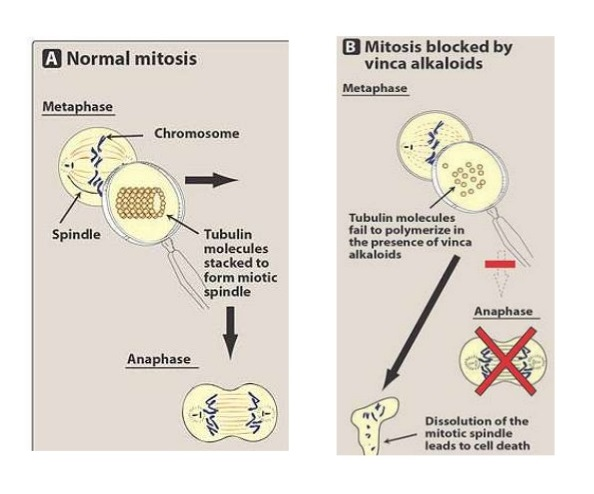
\includegraphics[width=.8\textwidth]{images/vincristine_mechanism}
  \caption{}
  \label{fig:vinchristine_mechanism}
\end{subfigure}
\caption[The structure and mechanism of Vincristine]{(a) The molecular structure of Vincristine. (b) Visualization of Vincristine's mechanism of action. During normal metaphase, microtubuli elongate from centrosome towards cell equator while pulling apart fully replicated chromosomes. Vincristine and other vinca alkaloids prevent this from happening by competitive inhibition, allosteric inhibition and active depolymerization of extending microtubuli. Unsuccessful exit from the metaphase forces the cell to undergo programmed cell death.}
\label{fig:vincs}
\end{figure}

\subsubsection*{Daunorubicin}

Daunorubicin is initially isolated from bacterium \textit{Streptomyces peucetius} \cite{otten1990cloning, lin2011chiral}. It is part of the anthracycline class of drug \cite{gewirtz1999critical} extracted mainly from \textit{Streptomyces} bacteria. Some well-known members of this class are Doxorubicin \cite{nci2018defdoxorubicin}, Epirubicin \cite{nci2018defepirubicin} and Idarubicin \cite{nci2018defidarubicin}. Together, they are among the most effective cancer drugs ever deployed and are used towards more kinds of cancer than other group of chemotherapeutic agents \cite{weiss1992anthracyclines, minotti2004anthracyclines, peng2005cardiotoxicology}. Like many chemotherapeutic agents including Vincristine, anthracyclines attack cancerous tissues and cells by preventing their division \cite{drugs2018defdaunorubicin}. Unlike vinca alkaloids however, anthracyclines prevent the division by disrupting another mechanistic part of cell division: the DNA polymerization \cite{gewirtz1999critical}. There are four ways anthracyclines disrupt DNA polymerization:

\begin{itemize}
\item Anthracyclines intercallate with base pairs involved in DNA polymerization thus preventing the extension of DNA strands \cite{takimoto2008principles}.

\item Anthracyclines covelatently inhibit type II topoisomerase which is responsible for RNA and DNA supercoil relaxation \cite{wang2002cellular}. Inhibition of type II topoisomerase causes supercoiled RNA and DNA to be inaccessible for initiation of duplication thus breaking the DNA \cite{tewey1984adriamycin}.

\item Anthracyclines induce oxidative stress on cancer cell organelles by generating free oxygen radicals. These radicals in turn damage DNA, proteins and cell membranes and initiate Caspase induced apoptosis \cite{vsimuunek2009anthracycline, halliwell1994free}.

\item Anthracyclines disrupt epigenetic, transcriptomic and DNA upstream regulations by removing histones from DNA strands \cite{pang2013drug}. This also exposes DNA strands to degradation factors such as DNA methylase \cite{vaissiere2008epigenetic} and oxidative damage \cite{ljungman1992efficient}

\item In the presence of formaldehyde, anthracyclines cross-link with the DNA covalently, creating cytotoxin that will disrupt DNA from functioning properly \cite{wang1991formaldehyde}.
\end{itemize}

In normal chemotherapeutic regimes, both Vincristine and Daunorubicin are prescribed intravenously to patients \cite{skeel2011handbook}. Needless to say, both drugs will disrupt both cancerous and healthy cells. The effect is however mostly felt in actively dividing cells and organs such as blood cells and hair follicles due to chemotherapeutic agents' highly disruptive effect during cell division as mentioned above \cite{skeel2011handbook, mayo2018chemotherapy}.

\begin{figure}[H]
\begin{subfigure}{.55\textwidth}
  \centering
  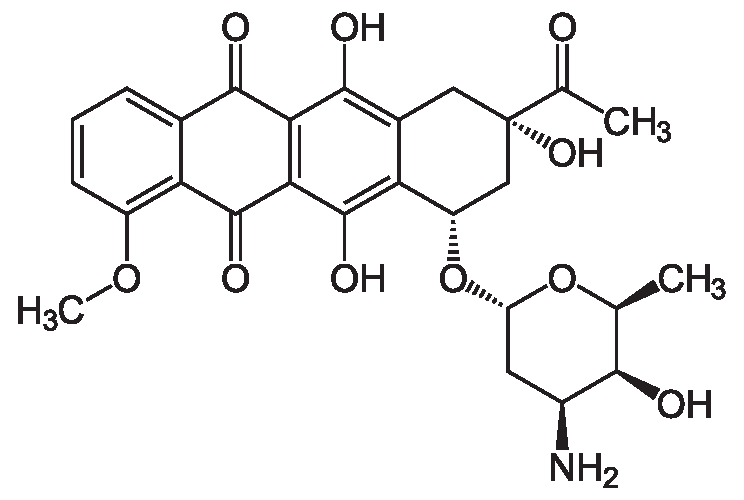
\includegraphics[width=\textwidth]{images/daunorubicin}
  \caption{}
  \label{fig:dauno}
\end{subfigure}
~
\begin{subfigure}{.4\textwidth}
  \centering
  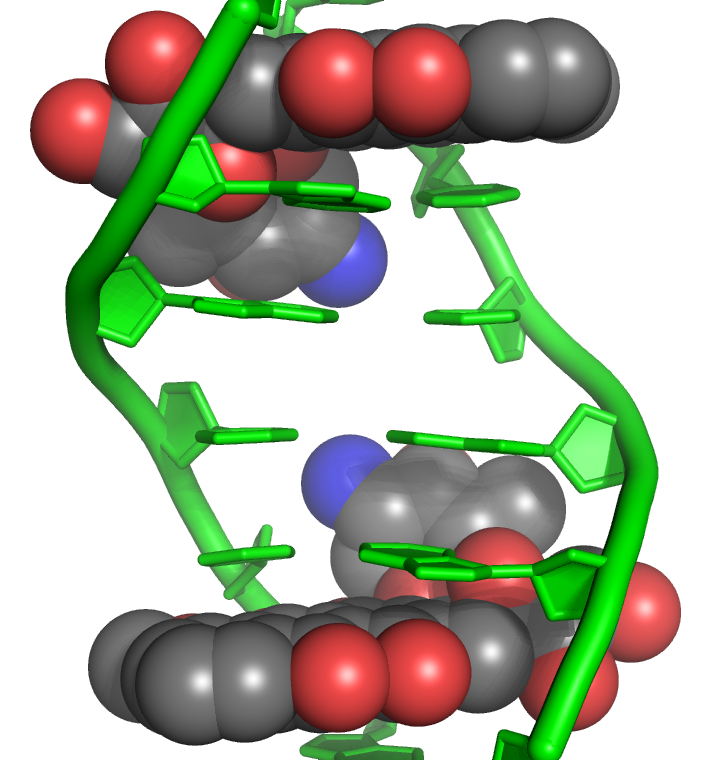
\includegraphics[width=\textwidth]{images/doxorubicin_dna}
  \caption{}
  \label{fig:anthracyclines_dna}
\end{subfigure}
\centering
\begin{subfigure}{\textwidth}
  \centering
  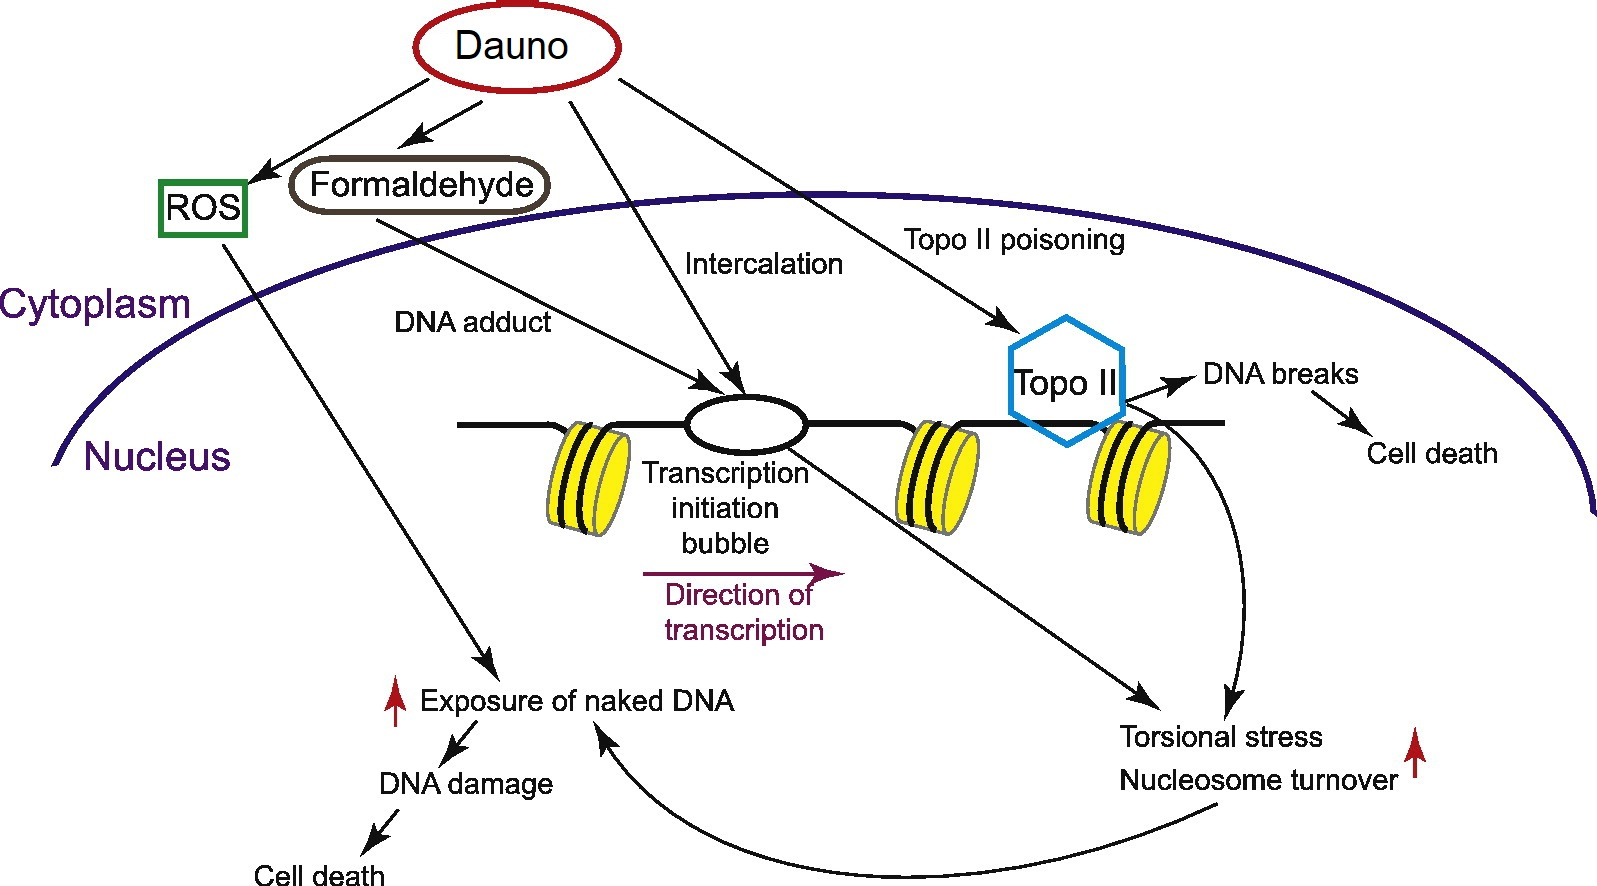
\includegraphics[width=\textwidth]{images/daunorubicin_mechanism}
  \caption{}
  \label{fig:dauno_mechanism}
\end{subfigure}
\caption[The structure and mechanism of Daunorubicin]{(a) The molecular structure of Daunorubicin. (b) Two anthracyclines intercalating with DNA double helix. (c) Schematic diagram of Daunorubicin's mechanism of action. From left to right: daunorubicin induces reactive oxygen species (ROS) which damage the DNA. Daunorubicin interfers with the DNA by (1) covalently crosslinking with the DNA mediated by formaldehyde and (2) intercalating DNA double helix. Daunorubicin also inhibits Topoisomerase II which prevents DNA supercoil's relaxation. Not shown in image: daunorubicin removes histone (shown in yellow in image) disrupting epigenetic regulations. Modified from (Yang et al, 2014 \cite{yang2014doxorubicin})}
\end{figure}

\subsection{Cell death signal}
\label{subsection:cell_death_signal}

As mentioned in Subsection \ref{subsection:treatment}, the introduction of cancer treatment disrupts mitotic cell activities which in turn activates cell death pathways. Two biochemical signals are selected to observe cell death caused by the disruption of mitotic process: %Caspase3/7 and Propium Iodide (PI).

\subsubsection*{Caspase 3/7}

Caspase 3 and 7 are both known as executioner Caspases in programmed cell death pathways \cite{alberts2017molecular}. For the project CellEvent Caspase3/7 vial from ThermoFisher Scientific is used  \cite{thermofisher2018casp}. Besides Caspase 3/7, the treatment consists also of a four amino acid peptide (DEVD) conjugated to a nucleic acid binding dye. This cell-permeable substrate is intrinsically non-fluorescent, because the DEVD peptide inhibits the ability of the dye to bind to DNA. After activation of Caspase 3 or Caspase 7 in apoptotic cells, the DEVD peptide is cleaved, enabling the dye to bind to DNA and produce a bright, fluorogenic response.  It has excitation/emission maxima of 502/530 nm (see Figure \ref{fig:caspase_spectra}).

\begin{figure}[H]

\centering

\begin{subfigure}{0.4\textwidth}
  \centering
  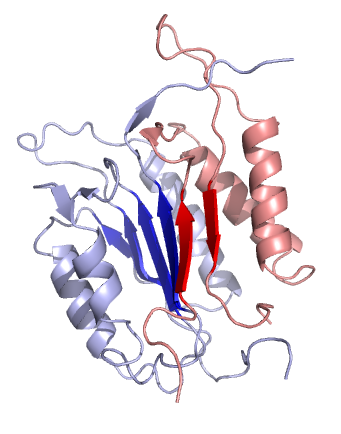
\includegraphics[width=\textwidth]{images/caspase3_dimer}
  \caption{}
  \label{fig:caspase3_dimer}
\end{subfigure}%
~
\begin{subfigure}{0.4\textwidth}
  \centering
  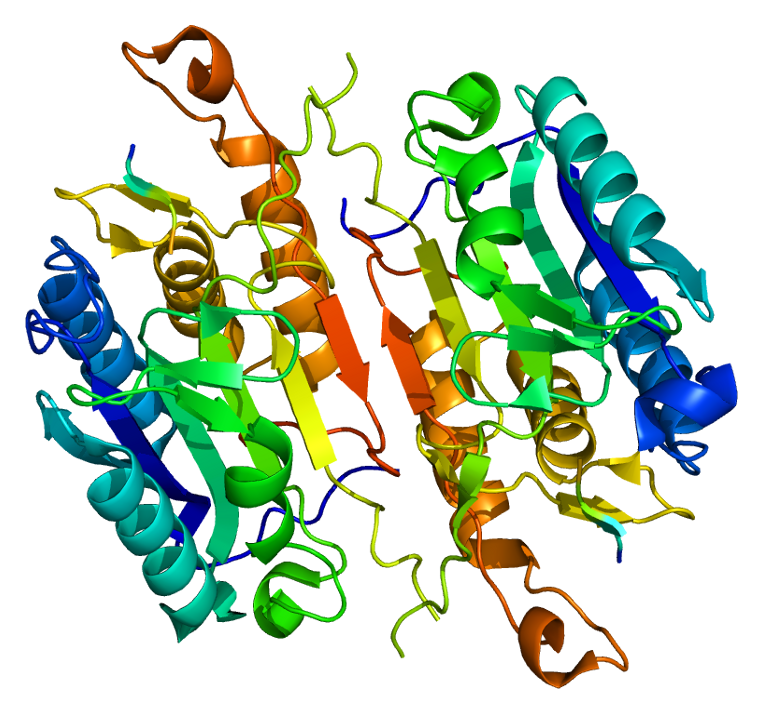
\includegraphics[width=\textwidth]{images/caspase7_dimer}
  \caption{}
  \label{fig:caspase37_dimer}
\end{subfigure}%

\centering

\begin{subfigure}{\textwidth}
  \centering
  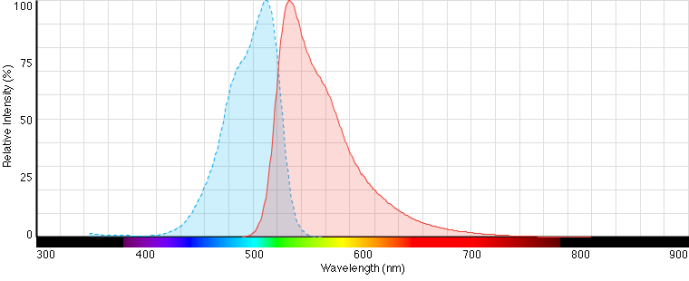
\includegraphics[width=0.8\textwidth]{images/caspase37_spectra}
  \caption{}
  \label{fig:caspase_spectra}
\end{subfigure}%

\caption[The structure and mechanism of Caspase 3/7]{(a) The molecular structure of Caspase 3 heterodimer (b) The molecular structure of Caspase 7 homodimer. The p17 (light blue) and p12 (pink) subunites are shown. (c) The excitation (blue) and emission (red) spectra of Caspase3/7 vial used in the experiment. Notice the emission peaking around the 525-535 nm range in green channel. Image taken from ThermoFisher Scientific product specification page \cite{thermofisher2018casp}.}

\label{fig:caspase_stain}
\end{figure}

\subsubsection*{Propium Iodide (PI)}

PI is membrane impermeable and generally excluded from viable cells. Therefore it is commonly used for identifying dead cells in a population and as a counterstain in multicolor fluorescent techniques. PI binds to DNA by intercalating between the bases with little or no sequence preference and with a stoichiometry of one dye per 4-5 base pairs of DNA \cite{suzuki1997dna}.  In aqueous solution, the dye has excitation/emission maxima of 493/636 nm (see Figure \ref{fig:pi_spectra}). PI also binds to RNA, necessitating treatment with nucleases to distinguish between RNA and DNA staining. Once the dye is bound to nucleic acids, its fluorescence is enhanced 20- to 30-fold. For the project PI vial from ThermoFisher Scientific is used \cite{thermofisher2018pi}.

\begin{figure}[H]
\centering

\begin{subfigure}{0.4\textwidth}
  \centering
  
\includegraphics[width=\textwidth]{images/pi}
  \caption{}
  \label{fig:pi_molecule}
\end{subfigure}%
~
\begin{subfigure}{0.6\textwidth}
  \centering
  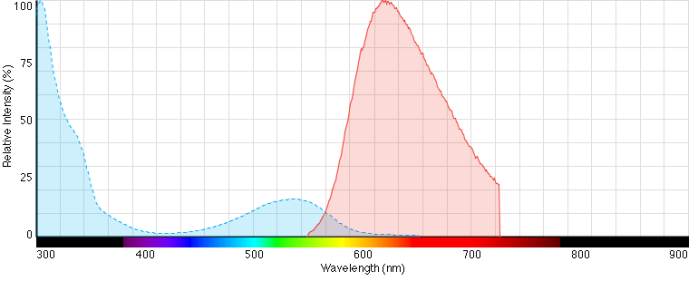
\includegraphics[width=\textwidth]{images/pi_spectra}
  \caption{}
  \label{fig:pi_spectra}
\end{subfigure}%

\caption[The structure and mechanism of Propium Iodide (PI)]{a) The molecular structure of Propium Iodide (PI) (b) The excitation (blue) and emission (red) spectra of PI. Notice the peaking around the 630-650 nm range in red channel. Image taken from ThermoFisher Scientific product specification page \cite{thermofisher2018pi}.}

\label{fig:pi_stain}
\end{figure}

\subsection{Experiment setup and image capturing}
\label{subsection:exp_setup}

In this project, two experiments are done:

\subsubsection{Unsynchronized experiment.}

In the unsynchronized experiment, all 8 wells of the ibidi\textsuperscript{\textregistered} sticky-Slide 8 Well ('slide') are used with one micro-trench wafer in each well (see Subsection \ref{subsection:microfluid_env} for the description of the slide). Every well is poured with different concentrations of drugs. To cover a large concentration range, a logarithmic scale is used to select concentration starting with 1 nanomolar (nM) all the way to 1000 nM (see Table \ref{table:unsyn_treatments}). The use of a logarithmic scale is also in line with the logarithmic nature of many enzymatic and molecular processes in cell biology \cite{wilkinson1961statistical, savageau1969biochemical}. Following concentrations are used:  1 nM, 5 nM, 10 nM, 100 nM and 1000 nM of Vincristine; 10 nM and 100 nM of Daunorubicin; and no drug as control. The unsynchronized experiment concentration configuration can be seen in Table \ref{table:unsyn_treatments}. The recording lasts for 45 hours. After 21 hours of recording, the drug treatment is introduced into each well. Table \ref{table:image_capture_frequency} shows the image capturing frequency for each image type.

\begin{table}[H]
\centering
\begin{tabular}{| l | c |}
\hline
Condition & Positions \\
\hline
A1: 1000 nM - VCR & 1-8 \\
A2: 100 nM - VCR & 9-15 \\
A3: 10 nM - VCR & 16-23 \\
A4: 1 nM - VCR & 24-31 \\
B4: 10 nM - Dauno 32 & 32-39 \\
B3: 100 nM - Dauno & 40-47 \\
B2: 0 nM - VCR & 48-55 \\
B1: 5 nM - VCR & 56-63 \\
\hline
\end{tabular}
\caption{Configuration table of treatments for synchronized experiment}
\label{table:unsyn_treatments}
\end{table}

\begin{table}[H]
\centering
\begin{tabular}{| l | l | c |}
\hline
What & What for & $t$ \\
\hline
In-focus brightfield (BF) image & Sanity check, micro-trench masking & 30 minutes \\
Out-of-focus BF image & Image tracking, image analysis & 15 minutes \\
Red fluorescence channel (PI)& Image tracking, image analysis & 15 minutes \\
Green fluorescence channel (Csp3/7) & Image tracking, image analysis & 15 minutes \\
\hline
\end{tabular}
\caption{Image capture frequency of the experiment}
\label{table:image_capture_frequency}
\end{table}


\subsubsection{Synchronized experiment}

The main difference between unsynchronized and synchronized experiments is the synchronization step. This process involves arresting cell cycle with the so-called "double thymidine block" protocol \cite{harper2005synchronization}, which arrests cell development at $G_1/S$-phase by stopping DNA synthesis using double thymidine block, a well known DNA synthesis inhibitor \cite{bostock1971evaluation}.

Like in the unsynchronized experiment, several concentration levels are tested in this experiment (see Table \ref{table:syn_treatments}). The image capturing starts right after the cells are synchronized and lasts 24 hours. The image capturing frequency is exactly the same as in the unsynchronized experiment (see Table \ref{table:image_capture_frequency}).

\begin{table}[H]
\centering
\begin{tabular}{| l | c |}
\hline
Condition & Positions \\
\hline
A1: 1000 nM - VCR & 1-8 \\
A2: 100 nM - VCR & 9-15 \\
A3: 10 nM - VCR & 16-23 \\
A4: 1 nM - VCR & 24-31 \\
B4: 0 nM & 32-39 \\
B3: 5 nM - VCR & 40-47 \\
B2: 10 nM - Dauno & 48-55 \\
B1: 100 nM - Dauno & 56-63 \\
\hline
\end{tabular}
\caption{Configuration table of drug treatments for synchronized experiment}
\label{table:syn_treatments}
\end{table}

\subsubsection{Image capturing}
\label{subsubsection:image_capturing}

Imaging was performed under an inverted Nikon Ti Eclipse microscope with a motorized stage (Tango XY Stage Controller, M\"arzh\"auser Wetzlar GmbH \& Co. KG, Germany), a CFI Plan Fluor DL 10X objective, a pco.edge 4.2 Camera (PCO AG, Kelheim, Germany) and a Lumencor Sprectra LED fluorescence lamp. For detection of the Caspase-3/7 and the PI marker, the following filters were used respectively, 474/27 nm, 554/23 (excitation) and 515/35 nm, 595/35 nm (emission). Brightfield out of focus (-20 $\mu$m) images were taken every 10 minutes and in-focus  brightfield and fluorescence images every 30 minutes for 48 hours. Vincristine or Daunorubicin were added after 20 hours from the beginning of the imaging. During the recording samples were kept at a constant temperature of 37\degree C and CO2 using an Okolab heating and CO\textsubscript{2} 2 box (OKOLAB S.R.L., NA, Italy). For the synchronized population, the double thymidine block protocol was followed. Briefly, MOLM-13s cells at the exponentially growing phase were incubated in blocking medium (culture medium supplemented with 2 mM Thymidine (CAS 50-89-5, Calbiochem\textsuperscript{\textregistered}, Germany)) for 24 hours. Cells were then released and incubated in culture medium for 8 hours and finally were incubated in blocking medium for 12 hours. After 2 hours, the synchronized population was seeded in the slide bearing the micro-trenches together with the markers and drugs at the same conditions as the unsynchronized population, and imaged for 24 hours.


\section{Definitions}

This section contains formal definitions and methods used in this thesis.

\subsection{Image channels and encoding}
\label{subsection:image_encoding}

Several image standards and encodings are being processed in our pipeline. We start from the raw image captured by the camera going down to processed images (See Subsubsection \ref{subsubsection:image_capturing} for detailed protocols on image acquisition). There are two brightfield channels (in-focus and out-of-focus channel) and two fluoroscent channels (red and green) in this project. Out-of-focus brightfield images are used to track cells as their unsharpness can be exploited through image processing creating robust patch of cells, as shown by Buggenthin \cite{buggenthin2011computational}. The red and fluoroscent channels capture fluorescence emission in 620-750 nm and 495-570 nm respectively (see Subsection \ref{subsection:cell_death_signal}).

\begin{itemize}
\item In-focus brightfield image, the focal distance of the camera $d_f$ is exactly the same as the distance of the camera to the center of the cell $d_m$, i.e. $d_f = d_m$.

\item In out-of-focus brightfield image, the difference of focal plane and center of the cells, $d_f - d_m$, influences the quality of the image in several ways (see Figure \ref{fig:focustest}). It was determined that the ideal image for segmentation came from the setting with $d_f - d_m = -20 \mu m$.

\item The red fluoroscent channel is used to capture emission from PI activation due to PI's DNA binding emission (see Subsection \ref{subsection:exp_setup}).

\item The green fluoroscent channel is used to capture emission from caspase3/7 activation due to DAVD peptide cleavage (see Subsection \ref{subsection:exp_setup}).
\end{itemize}

%TODO change image labeling

\begin{figure}[H]
\centering
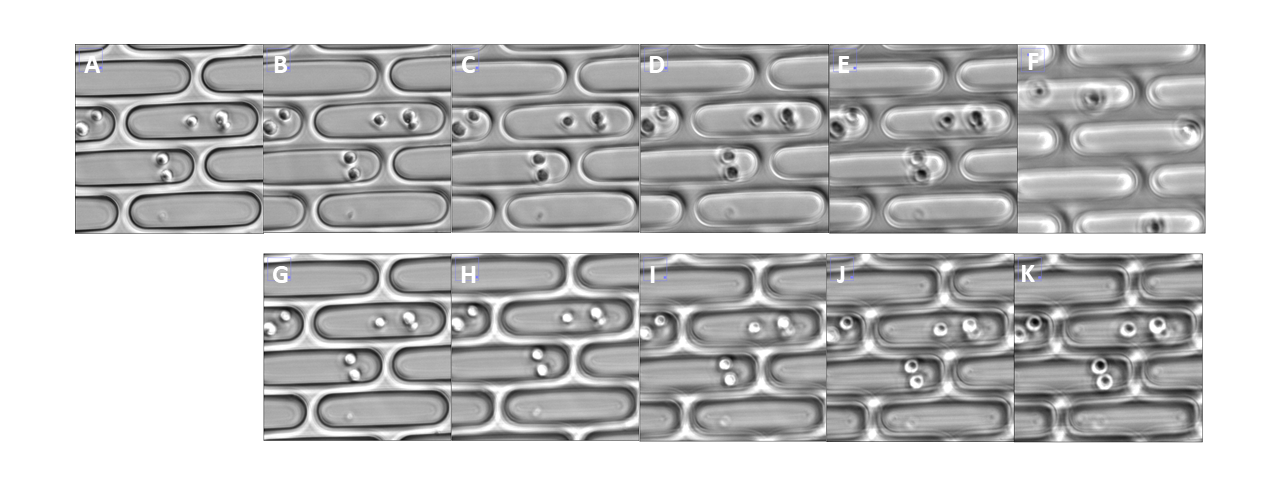
\includegraphics[width=\textwidth]{images/focus/pict.png}
\caption[Effect on focal plane on out-of-focus image]{In-focus image and out-of-focus brightfield images taken at various focus levels.  In the first row are images focused behind the microfluidics system while in the second row are images focused before the system. A: in focus image. B: $+10 \mu m$. C: $+20 \mu m$. D: $+30 \mu m$. E: $+40 \mu m$. F: $+50 \mu m$. G: $-10 \mu m$. H: $-20 \mu m$. I: $-30 \mu m$. J: $-40 \mu m$. K: $-50 \mu m$.}
\label{fig:focustest}
\end{figure}

The camera records TIFF images (see Appendix \ref{appendix:imageacquisition} for the detailed protocols) \cite{loc2006tiff}. Each recorded stack consists of slice with one slice representing a single image capture at a time point. Each stack is encoded using RGB color model. This is also the case for the fluorescent image in which each slice shows the intensity in corresponding color channel (red, green or blue) as a monochromatic RGB image.

RGB color model represents the pixel as a combination of red, green and blue color. This encoding is able to represent any human visible color and is useful enough for most use cases \cite{sonka2014image, jayant1993signal}. The most commonly used RGB encoding is the 8 bit encoding. Here, each pixel is represented as an RGB pixel having red, green and blue color values ranging from 0 to 255. Mathematically, this means that each pixel $M_{t,x,y}$ of a slice captured at time $t$ can be represented as a triple, i.e.,

\begin{equation}
\label{equation:rgb_pixel_def}
M_{t, x, y} := (M_{t, x, y, R}, M_{t, x, y, G}, M_{t, x, y, B}) \in [0:255]^3
\end{equation}

for 8-bit RGB encoding. Consequently, a slice $M_t$ captured at time $t$ of width $w$ and height $h$ is a 3-dimensional matrix of dimension $w \times h$, i.e.

$$
M_i \in p_c^{w \times h \times 3}
$$ 

with $p_c \in [0:255]$. A stack (a sequence of slices) $M$ of $n$ slices is in turn a 4-dimensional matrix:

$$
Mw \in p_c^{n \times w \times h \times 3}
$$ 

To convert the RGB value of a pixel $M^a_{x,y}$ from one bit-encoding to another $M^b_{x,y}$, linear conversion is used:

\begin{equation}
\label{equation:linear_conv_rgb}
M^b_{x,y} = (\lceil M^a_{x,y, 1} \frac{2^b}{2^a} \rceil, \lceil M^a_{x,y, 2} \frac{2^b}{2^a} \rceil, \lceil M^a_{x,y, 3} \frac{2^b}{2^a} \rceil)
\end{equation}

where $a$ and $b$ refer to the bit length of the source and target encoding respectively (commonly known as bid depth).  Commonly used depths are 8, 16 (high color format), 24 (true color format) and 48 bits (deep color format) \cite{lim1990two, sharma1997digital, sullivan2012overview}.

Sometimes, other type of encodingsa like grayscale and 1-bit monochrome are used. A grayscale image essentially shows the intensity of the pixels in an image. A grayscale slice $G$ can be represented as a matrix of integer, i.e. $G \in p_c^{w \times h}$. Like RGB image, linear scaling can be applied to transform grayscale images across bit depth:

\begin{equation}
\label{equation:linear_conv_gray}
G^b_{x,y} = \lceil G^a_{x,y} \frac{2^b}{2^a} \rceil
\end{equation}

An RGB image can be transformed to a grayscale image by combining the intensity from every channel:

$$
G_{x, y} = \frac{M_{x, y, 1} + M_{x, y, 2} + M_{x, y, 3}}{3}
$$

This however does not reflect human perception of light, as human eyes' spectral sensitivity is not uniform across the color spectrum \cite{wyszecki1982color}. Indeed, as Osorio and Vorobyev shows in 2005, each species has its own specific spectral sensitivity distribution \cite{osorio2005photoreceptor}, as can be seen in following figure:

\begin{figure}[H]
\centering
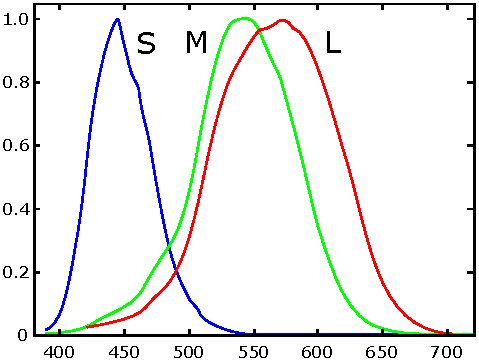
\includegraphics[width=0.5\textwidth]{images/spectral_sensitivity_human.pdf}
\label{fig:spectral_sensitivity}
\caption[Spectral sensitivity of human]{Spectral sensitivity of human. Note that the sensitivity distribution is maximum normalized. Each curve shows the relative sensitivity of each type of human cone cells (S, M and L types). The curve color represents the dominating absorbed color range of each cell type.}
\end{figure}

There are some conversions published on transforming RGB value to human intensity perception based on the measured spectral sensitivity \cite{anderson1996proposal, itu2007studio, itu2015parameter}. Among the most commonly used is the \textit{BT.601} standard from International Telecommunication Union (ITU). It recommends the following luminosity weight for RGB to grayscale conversion \cite{itu2007studio}:

\begin{equation}
G_{x, y} = \frac{0.299 M_{x, y, R} + 0.587  M_{x, y, G} + 0.114 M_{x, y, B}}{3}
\label{equation:rgb_to_gray_def}
\end{equation}

For following image: 

\begin{figure}[H]
\centering

\includegraphics[width=0.4\textwidth]{images/pos_41_in_t0}
\caption{The in-focus image position 41 from unsynchronized experiment.}
\label{fig:pos41}
\end{figure}

using Equation \ref{equation:rgb_to_gray_def} to convert RGB to intensity , we can convert the image into grayscale image representing the intensity. The grayscale image has the intensity distribution as shown in following histogram:

\begin{figure}[H]
\centering
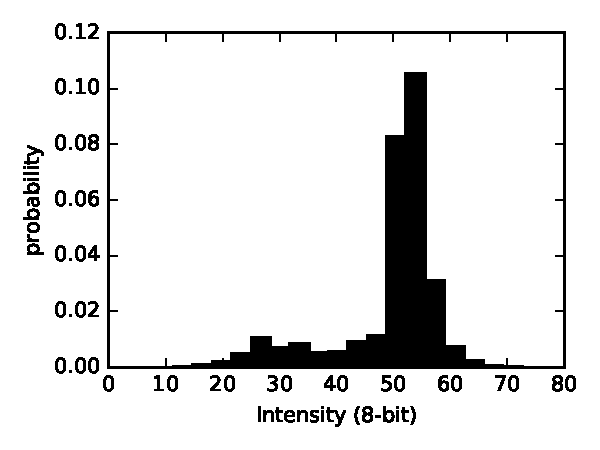
\includegraphics[width=0.4\textwidth]{images/pos_41_in_t0_hist}
\caption{Normalized distribution of intensity of Figure \ref{fig:pos41}.}
\label{fig:pos41_density}
\end{figure}

Reverting back a grayscale image to an RGB image in turn only consists of applying grascale value to each color component:

$$
M_{x, y} := (G_{x, y}, G_{x, y}, G_{x, y})
$$

A 1-bit monochrome image is encoded as a binary matrix:

$$
B \in p_b^{w \times h} \land p_b \in \{0, 1\}
$$

This encoding is useful when not using not the complete information of the image but rather separation of interesting parts in the image, since since it requires less memory (1 bit per pixel vs 24 bits per pixel of normal RGB image) and enables bitwise operation of the CPU which takes constant time \cite{kernighan1988c}.  Some use cases are for example region of interest (ROI) bounding and contour and boundary visualization \cite{hartley2003multiple}.

The conversion from RGB to binary images can be done by defining a cutoff value $c$ on one of the channels, e.g. for red channel, following conversion can be used:

\begin{gather*}
B_{x, y} =
\begin{cases}
  1 & \text{if } M_{x, y, R} > c\\    
  0 & \text{else}  
\end{cases}
\end{gather*}

Note that, a bit encoding of an image refers to unsigned encoding. Thus, an $m$-bit encoding allows value ranging from $0$ to $2^m - 1$.

\subsection{Intensity, brightness and contrast}
\label{subsection:brightness_contrast_adjustment}

Intensity, brightness and contrast can be modified to show and hide parts of an image. In this project, many image processing steps utilize the modification of them. Previously we defined  intensity in image encoding. In this subsection we will define brightness and contrast and their adjustment.

Mathematically, we can represent brightness and contrast adjustment as a mapping between one domain to another. Let $l(M_{t, i, j})$ be a function that maps the RGB value of a pixel $M_{t, i, j}$ to its corresponding intensity $I_t$. Conventiently, we can use ITU's \textit{BT.601} standard formula written in Subsection \ref{subsection:image_encoding} to convert an RGB to grayscale image.

We then define the $I_t: [0:w] \times [0:h] \rightarrow \mathbb{N}_0$ function that maps the coordinate of a pixel to its corresponding intensity value i.e.

$$
I_t(i, j) := l(M_{t, i, j})
$$

Note that the codomain of the function $I_t$ depends on the encoding used. For a 8-bit encoding this will be then $[0:255]$.

An intensity transformation $J_t$ is then defined as a linear transformation of $I_t$ with \textbf{gain} and \textbf{bias} parameters $\alpha$ and $\beta$ respectively:

\begin{equation}
\label{equation:br_ct_transform}
J_t(i, j) := \alpha \cdot I_t(i, j) + \beta
\end{equation}

with $\alpha > 0$ \cite{szeliski2010computer}. The gain and bias parameters are also known as \textbf{contrast} and \textbf{brightness} parameters. In this regard, increasing/decreasing brightness is equivalent to increasing/decreasing $\beta$. The same thing also applies for contrast parameter, increasing $\alpha$ will increase the contrast of the image.

Predictably, doing transformation using transformation function $J_t$ will inevitably cause the resulting intensity to be outside of the allowed value range $[0:2^m]$ for m-bit encoding. To understand this situation, we first have to consider the boundedness of eyes perception. The argumentation for boundedness can be shown by realizing that the excitation of a neuron follows a sigmoid function \cite{gazzaniga2004cognitive}. Thus given no impuls the neuron will stay in ground state, while very large impulse is bounded due to biochemical constraint of a neuron. Mapped in the context of a sigmoid function, a steady state corresponds to 0 while asymptotically unlimited excitation corresponds to 1. In our context, a non-excited state corresponds to 0 intensity while full-excitation corresponds to $2^m - 1$ intensity. Thus, the Equation \ref{equation:br_ct_transform} can be bounded by introducing upper and lower bounds of $0$ and $2^m - 1$, i.e.

\begin{gather*}
J_t(i, j) :=
\begin{cases}
  2^m - 1 & \text{if } \alpha \cdot I_t(i, j) + \beta > 2^m - 1\\
  0 & \text{if } \alpha \cdot I_t(i, j) + \beta < 0\\
  \alpha \cdot I_t(i, j) + \beta & \text{else}
\end{cases}
\end{gather*}

We can for example, transform Figure \ref{fig:pos41} using $J_t(i, j)$ with $\alpha = 1$ and $\beta=100$. The transformed image can be seen in Subfigre \ref{fig:pos41_brup100_bf} with Subfigure \ref{fig:pos41_brup100_hist} shows the intensity distribution of the transformed image. We can also try to modify $\alpha$. Changing $\alpha$ to a value larger than 1 will scale the image's intensity and emphasize/de-emphasize image contrast. Subfigure \ref{fig:pos41_brup100_hist} shows the transformed image for $\alpha = 3$ and $\beta  = 0$.

See for example following image:

\begin{figure}[H]
\centering

\begin{subfigure}{0.4\textwidth}
  \centering
  
\includegraphics[width=\textwidth]{images/pos_41_in_t0_br_up100}
  \caption{1a}
  \label{fig:pos41_brup100_bf}
\end{subfigure}%
~
\begin{subfigure}{0.4\textwidth}
  \centering
  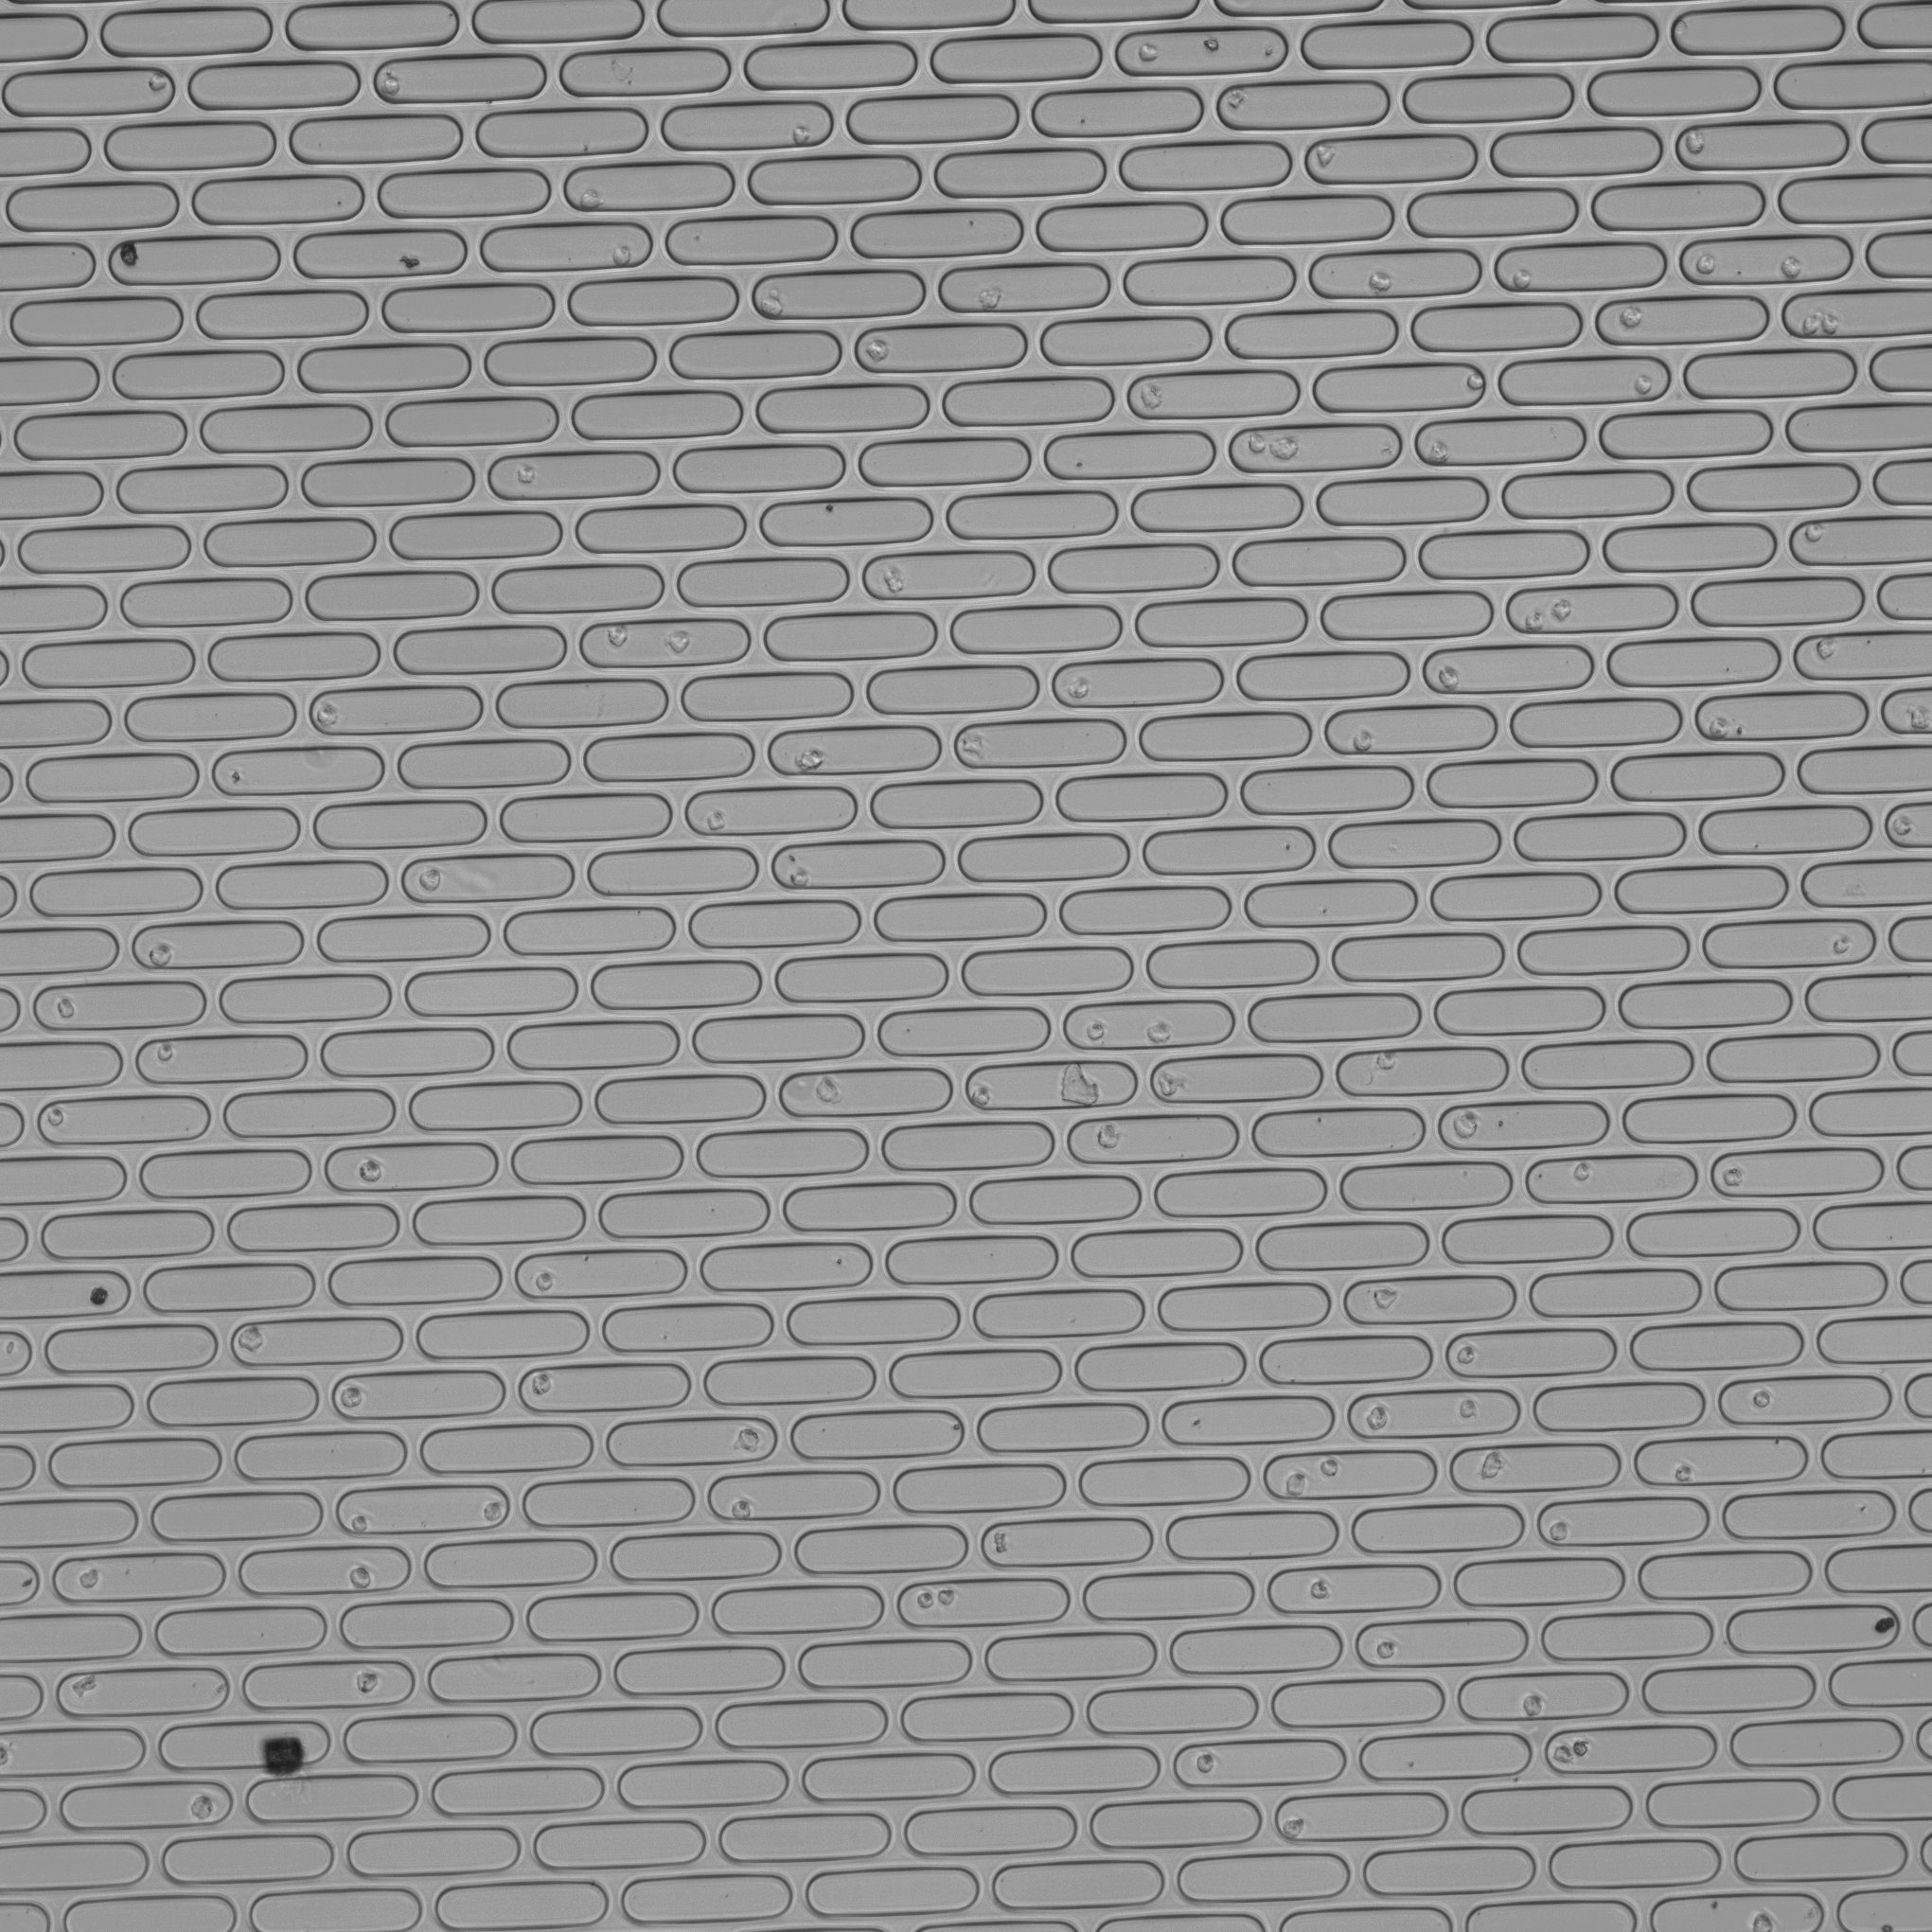
\includegraphics[width=\textwidth]{images/pos_41_in_t0_br_times3}
  \caption{}
  \label{fig:pos41_times3_bf}
\end{subfigure}%

\centering

\begin{subfigure}{0.4\textwidth}
  \centering
  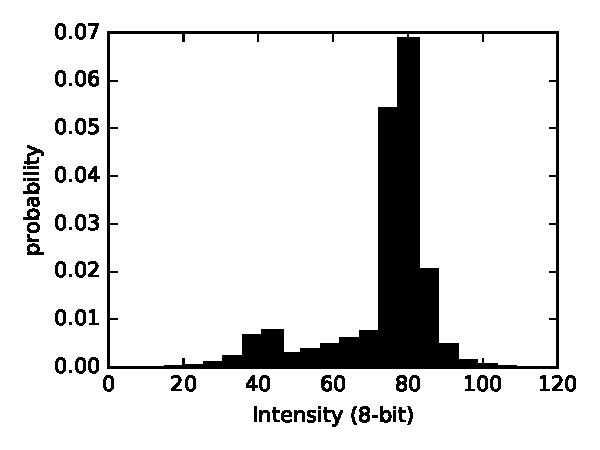
\includegraphics[width=\textwidth]{images/pos_41_in_t0_br_up100_hist}
  \caption{}
  \label{fig:pos41_brup100_hist}
\end{subfigure}%
~
\begin{subfigure}{0.4\textwidth}
  \centering
  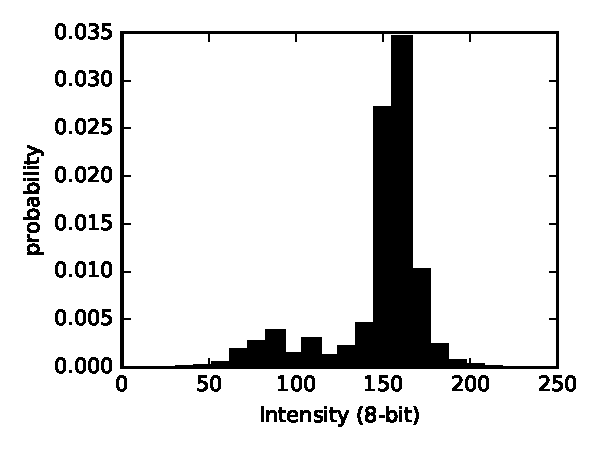
\includegraphics[width=\textwidth]{images/pos_41_in_t0_br_times3_hist}
  \caption{}
  \label{fig:pos41_times3_hist}
\end{subfigure}%

\caption[Brightness and contrast transformation]{(a) The in-focus image position 41 from unsynchronized experiment transformed with $\alpha=1$ and $\beta = 100$. (b) The in-focus image of position 41 from unsynchronized experiment transformed with $\alpha=3$ and $\beta = 0$. Notice the contrast has increased significantly, especially around area with high intensity differential such us the margin of a micro-trench and the dark spot in the lower left part of the slice. (c) Normalized distribution of intensity of (a). (d) Normalized distribution of intensity of the (b). Note that the difference in height across bins in two histograms is mainly caused by the definition of bins in the histogram function.}

\label{fig:pos41_brup100}
\end{figure}

Geometrically, brightness describes the level of visibleness of a pixel. Adjusting $\beta$ shifts the entire intensity distribution to the right by $\beta$ \footnote{Note the wording. For negative $\beta$, the shift is negative to the right, i.e. to the left}. On the other hand, contrast can be understood as the distance of closely resembling pixel \cite{hartley2003multiple}. Two pixels which are very similar will look very different given a high contrast.

\subsection{Robust automatic threshold selection (RATS)}
\label{subsubsection:rats}

Robust Automated Threshold Selection (RATS), based on description by Wilkinson and Schut\cite{wilkinson1998digital}, computes a threshold map for an image based on two criteria: pixel values, and pixel gradients \cite{fiji2017rats}.

The gradient is computed using the so-called Sobel kernel \cite{sobel1990isotropic} a commonly used in computer vision for edge detection as it particularly emphasizes edges in an image upon transformation. It is a discrete differential operator which computes an approximation of the gradient of the intensity function $J$.

Originally, the Sobel gradient $\mathbb{G}_{x, y}$ of coordinate $(x, y)$ is defined as

$$
\mathbb{G}_{x, y} := \sqrt{\Delta_x^2 + \Delta_y^2}
$$

Whereas $\Delta_x$ and $\Delta_y$ are defined as

\[
\Delta_x = 
\begin{bmatrix}
+1 & 0 & -1 \\
+2 & 0 & -2 \\
+1 & 0 & -1 \\
\end{bmatrix}
*
\mathbf{M_t}
\]

and

\[
\Delta_y = 
\begin{bmatrix}
+1 & +2 & +1 \\
+0 & 0 & 0 \\
-1 & -2 & -1 \\
\end{bmatrix}
*
\mathbf{M_t}
\]

with $\mathbf{M_t}$ denoting the image at time $t$ and asterisk symbol $*$ denotes  a two dimensional signal processing convoltion \cite{smith1997scientist}. For example, for a $3 \times 3$ matrix,

\[
X_{3 \times 3} = 
\begin{bmatrix}
1 & 2 & 3 \\
4 & 5 & 6 \\
7 & 8 & 9 \\
\end{bmatrix}
\]

and $\Delta_x$, the value of the middle pixel $(2, 2)$ after evaluating the convolution $\Delta_x * X_{3 \times 3}$ is,

\[
\left( 
\begin{bmatrix}
+1 & 0 & -1 \\
+2 & 0 & -2 \\
+1 & 0 & -1 \\
\end{bmatrix}
*
\begin{bmatrix}
a & b & c \\
d & e & f \\
g & h & i
\end{bmatrix}
\right) [2,2]
= i \cdot 1 + 0 \cdot h - 1 \cdot g + 2 \cdot f + 0 \cdot e - 2 \cdot d - 1 \cdot g + 0 \cdot h - 1 \cdot a
\]

It has been shown, however, that only taking the quadratic gradient yields comparable result \cite{wilkinson1998digital}. The Sobel operator is thus defined as quadratic gradient in Fiji RATS plugin, i.e.

$$
\mathbb{g_{x, y}} = \mathbb{G_{x, y}^2}
$$

Pixels having gradients smaller than threshold $\lambda \sigma$ are then removed, where $\sigma$ is the noise (generally, standard deviation of the expected background is used, e.g. standard deviation of the whole image) and $\lambda$ is the scaling factor (Wilkinson determined $\lambda = 3$ to be a good approximation \cite{wilkinson1998digital}). Visually, this step can be understood as removal of background noise from the image.

To refine the filtering further, iterative correction is applied. First, a quadtree construction is applied in an image. A quadtree is a tree-like data structure in which each node has exactly four children (Finkel and Bentley, 1974 \cite{finkel1974quad}). In the context of an image, an image is recursively separated into smaller quadtree until the standard deviation of the intensity in every quadtree is lower than a pre-defined limit (usually the standard deviation of the intensity of the whole image $\sigma$). Figure \ref{fig:quadtree} gives an example on how a quadree is constructed from an image.

\begin{figure}[H]
\centering
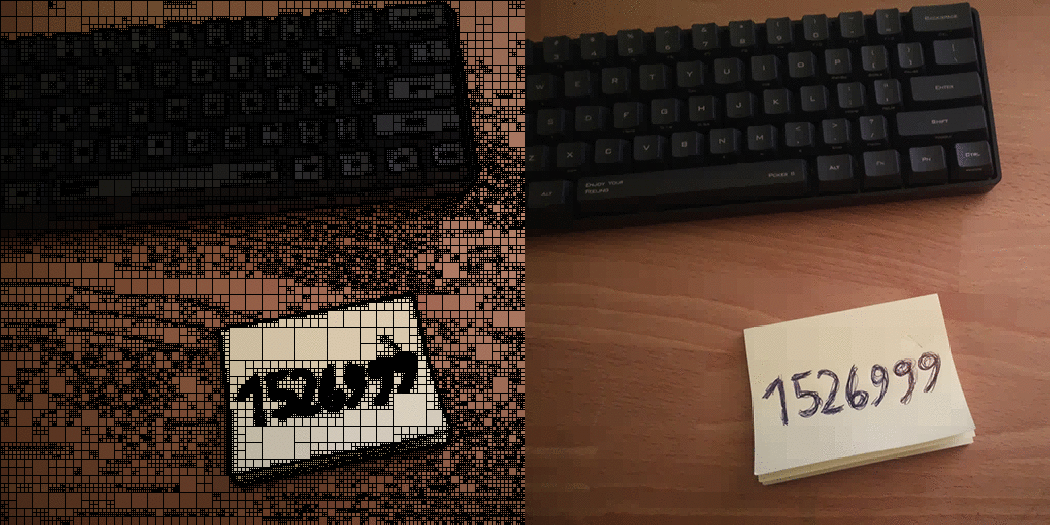
\includegraphics[width=0.8\textwidth]{images/quadtree}
\caption[Example of quadtree]{Example of quadtree. The left side is the quadtree representation of original image on the right. \textit{Creative Commons courtesy of anonymous.}}
\label{fig:quadtree}
\end{figure}

In the second step, we attempt to remove the filter locally. To do that, we first define a local threshold $T_R$ within the smallest square. For a quadrant, the threshold is computed in following way:

\begin{equation}
T_R = \frac{\sum g_{x,y} \cdot M_{t, x, y}}{\sum g_{x, y}}
\label{eq:local_threshold_rats}
\end{equation}

Where $\sum g_{x,y}$ the sum of all children quadrants' gradient. For the smallest quadrant, only $g_{x,y}$ is used instead, i.e.

\begin{equation}
T_R = \frac{g_{x,y} \cdot M_{t, x, y}}{g_{x, y}}
\label{eq:local_threshold_rats_smallest}
\end{equation}

This threshold is used to filter pixels within a quadrant. Pixels with gradient value smaller than $T_R$ of a quadrant are then filtered out. If $T_R$ is very low that no point in a quadrant is filtered out, the $T_R$ of the parent is taken instead. This step is iterated until a parent square with at least one filtered pixel is reached. Visually, the refining step is equal to filtering out the area of an image in which the pixels are mostly noise. In the initial global filtering process, many noisy pixels might not be filtered since they happen to have gradients larger than $\lambda \sigma$. Using this bottom-up approach these pixels will be eventually filtered out.

\subsection{Holes filling}
\label{subsection:holes_filling}

Filling micro-trench holes to create the contour is done in two steps:

\begin{enumerate}
\item Recognition of the outer part of micro-trench contours, followed by
\item Filling of such contour with a new neutral value (black).
\end{enumerate}

Following image explains the definition of contours and their hierarchy:

\begin{figure}[H]
\centering
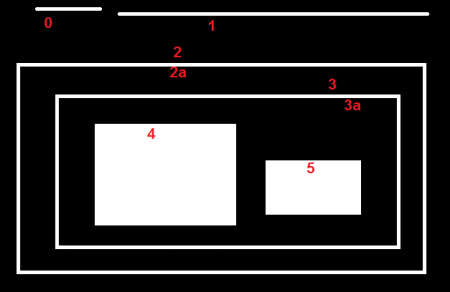
\includegraphics[width=0.8\textwidth]{images/contours}
\caption[Example of image contours]{Example of contours and their hierarchy. \textbf{Contours 0}, \textbf{1} and \textbf{2} are \textbf{outernmost contours} and of \textbf{hierarchy-0}. \textbf{Contour 2a} is \textbf{child contour} and of \textbf{hierarchy-1}. \textbf{Contour 3} is child contour of \textbf{contour 2a} and of \textbf{hierarcy-2}. \textbf{Contour 3a} is child contour of  \textbf{contour 3} and of \textbf{hierarchy-3}. Both \textbf{contours 4} and \textbf{5} are children of \textbf{contour 3a} and of \textbf{hierarchy-4}. All contours with same hierarchy are topologically equal. Contour Adopted from OpenCV tutorials by Bradski and Kaehler \cite{bradski2008learning}.}
\label{fig:contours}
\end{figure}

There are several well known algorithms for hierarchical contours recognition. In our case, the algorithm of Suzuki and Abe \cite{suzuki1985topological} is used. The algorithm works by walking along the border between two regions of different color. The border walking process is done hierarchically creating tree-like dependency structure of contours. We then take the outermost (hierarchically the highest) contours which are then filled. The filling in turn is simply done by assigning neutral value in every pixel located inside every outermost contour.

%TODO add similar image to analytic pipeline
%\begin{figure}[H]
%\centering
%\begin{subfigure}{\textwidth}
%  \centering
%  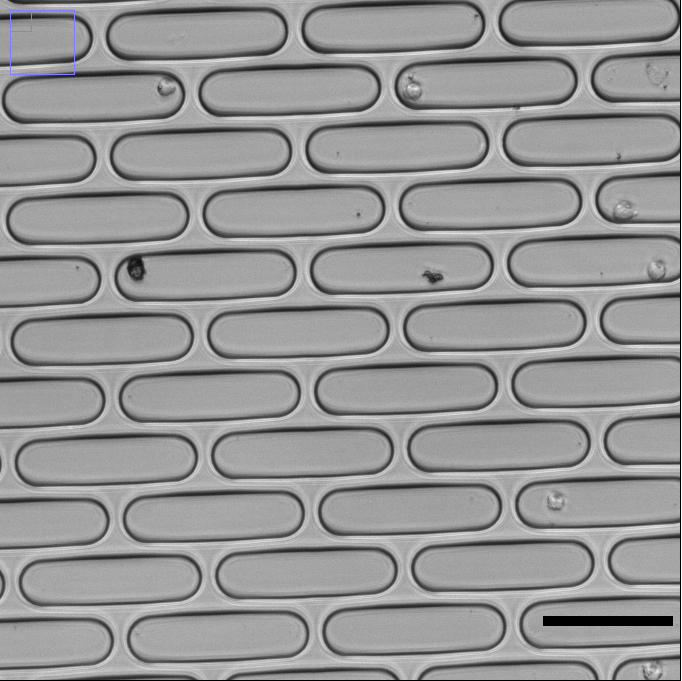
\includegraphics[width=0.28\textwidth]{images/trench_detect_1}
%  \caption{}
%  \label{fig:orig_pic}
%\end{subfigure}%
%\begin{subfigure}{\textwidth}
%  \centering
%  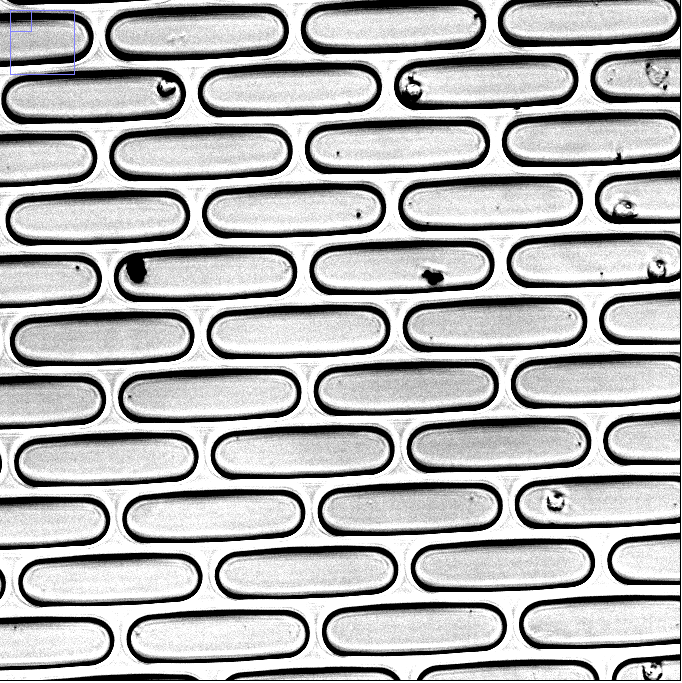
\includegraphics[width=0.28\textwidth]{images/trench_detect_2}
%  \caption{}
%  \label{fig:brcon_adj}
%\end{subfigure}%
%\begin{subfigure}{\textwidth}
%  \centering
%  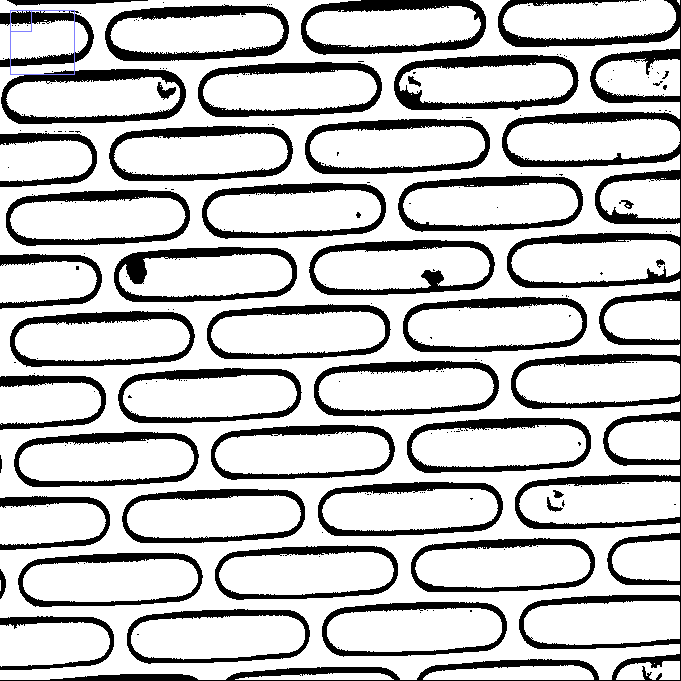
\includegraphics[width=0.28\textwidth]{images/trench_detect_3}
%  \caption{}
%  \label{fig:rats}
%\end{subfigure}%
%\begin{subfigure}{\textwidth}
%  \centering
%  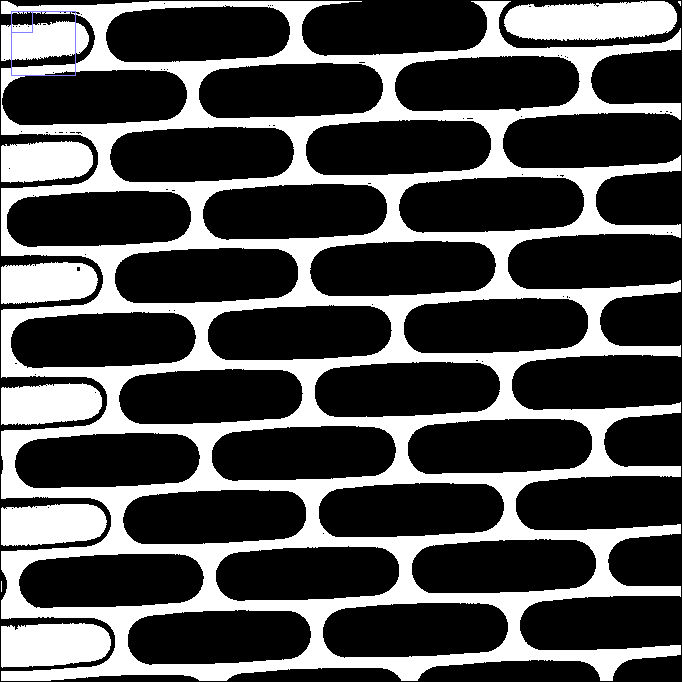
\includegraphics[width=0.28\textwidth]{images/trench_detect_4}
%  \caption{}
%  \label{fig:fill_holes}
%\end{subfigure}%

%\caption[Micro-trenches masking process]{The upper left corner of the image position 41's in-focus-image recording at time $t=0$: (a) The original in-focus image of the upper left corner of  the image position 41. (b) The view of the same area as (a) after applying brightness and contrast adustment. (c) The view of the same area after applying RATS on image in (b) showing the contour of micro-trenches in the area. (d) The contours filled with neutral color (black). Note that some micro-trenches are not filled as they are open and thus topologically not the outernmost contours. Scale bar on the uppermost figure is $100 \mu M$ long.}
%\label{fig:trench_masking}
%\end{figure}

\subsection{Gaussian blur}
\label{subsection:gaussian_blur}

Gaussian blurring in the context of image processing is the process of applying a Gaussian noise on an image. The Gaussian function $G: \mathbb{R} \rightarrow \mathbb{R}$ is a function defined as

$$
G(x) = \frac{1}{\sqrt{2\pi \sigma^2}} e^{-\frac{x^2}{2 \sigma^2}}
$$

In 2 dimensional setting, we extend the function to $G: \mathbb{R} \times \mathbb{R} \rightarrow \mathbb{R}$ defined as

\begin{equation}
G(x,y) = \frac{1}{{2\pi \sigma^2}} e^{-\frac{x^2 + y^2}{2 \sigma^2}}
\label{equation:gauss_2d}
\end{equation}

Applying this function on a 2D image creates concentric circles centered around the center of the distribution with values around the center distributed normally. This means that, for an arbitrary $\sigma$  and a uniform image with the intensity of $n$ in every pixel,  convolving the image with Equation \ref{equation:gauss_2d} centered at point $(i, j)$ yields a transformed image with the transformed intensity $I^G$ of each point distributed normally around $(i, j)$ with scaling of $n$ and standard deviation $\sigma$:

\begin{equation}
I^G(x, y) = n \cdot \frac{1}{{2\pi \sigma^2}} e^{-\frac{(x - i)^2 + (y - j)^2}{2 \sigma^2}}
\label{equation:gauss_intens_trans}
\end{equation}

The idea of transforming an image with one selected center point is however not very practical as the pixels far away from image will have intensity of almost zero. We can however, use the fact fact that the intensity of pixels around the center point fall exponentially the further the pixels are away to introduce a dependency of each pixel on its surrounding environment. This will introduce a blur due to pull-down effect of the neighboring pixels. Hence the name \textbf{Gaussian blurring}.

Mathematically, we can express the Gaussian blurring process as convolving the pixels around a pixel $(x, y)$ and take the average of the convoluted image as the new intensity value in $(x, y)$. Using the continuous Gaussian intensity transformation defined in Equation \ref{equation:gauss_intens_trans}, the Gaussian convolution  function is defined as following:

$$
I^{conv_G}(x, y) = \frac{\sum_{x - \lfloor d/2 \rfloor < i < x + \lfloor d/2 \rfloor} \sum_{x - \lfloor d/2 \rfloor < j < x + \lfloor d/2 \rfloor} I^G(i, j)}{(\lfloor d/2 \rfloor)^2}
$$

with $d$ denoting the $L_1$ distance of the blur.  We can furthermore refine the convolution further by using $L_2$ distance (i.e. radius) instead:

\begin{equation}
I^{conv_G}(x, y) = \frac{\sum_{(i, j) \in C}  I^G(i, j)}{\| C \|}
\label{equation:conv_gaussian_cont}
\end{equation}

for $C := \{(i, j)  \text{  where } d_{L_2}((x, y), (i, j)) \leq d\}$. It can be seen from the equation that increasing the radius $d$ increases the pull-down effect on the pixel and hence increases the smoothness of in the image. We exploit this property to create regional gradient which will be used to normalize an image by its background gradient. By dividing the value of each pixel by the convoluted value of it we can correct the image by its global background noise. The Gaussian blur-corrected intensity $I^{conv_G}$ is thus defined as

\begin{equation}
I^{c_G}(x, y) = \frac{I(x, y)}{I^{conv_G}(x, y)} 
\label{equation:gauss_blur_correction}
\end{equation}

Visually, the method can be understood as low pass filter. It removes the higher frequency 2D signals, i.e. the value with high local variance, resulting with an image with lower fidelity and local variance.

\subsection{Contrast limited adaptive histogram equalization (CLAHE)}
\label{subsection:clahe}

CLAHE, initially developed by Karel Zuiderveld in 1994 \cite{zuiderveld1994contrast}, is an instance of the class of algorithms called adaptive histogram equalization (AHE) commonly used to improve contrast in an image. An AHE algorithm generally works by transforming each pixel with a transformation function derived from the neighboring region instead of the whole image.  By doing this, an AHE algorithm can count for the variation of brightness and contrasts in areas of an image \cite{pizer1987adaptive}.

The distinction of CLAHE among other AHE algorithms is the contrast limiting property of the algorithm. Given a contrast distribution of an area around a given point, CLAHE conducts following steps:

\begin{enumerate}
\item First, the algorithm takes a predefined clipping value of the intensity histogram of the area around a center point.
\item The algorithm then calculates the intensity histogram of the area.
\item For some intensity values there will be more pixels than allowed with the intensity values. We call these intensity values the clipping intensity area.
\item Adapt the intensity histogram by reassigning the intensity of some pixels in the clipping intensity area uniformly across the range of intensity in the image (see upper part of Figure \ref{fig:clahe}).
\item Repeat until for randomly selected areas in the image the clipping value constraint is satisfied, i.e. for every randomly chosen pixel, the intensity histogram contains no clipping intensity area.
\end{enumerate}

Figure \ref{fig:clahe} visualizes the step 2, 3 and 4 of the algorithm description above. As can be seen in the area intensity CDF in the lower part of Figure \ref{fig:clahe}, the algorithm results in a more equalized distribution of intensity. Visually, this increases the contrast and in turn sharpens the image. Figure \ref{fig:clahe_before_after} shows an area of the well before and after the application of CLAHE. Note the increased brightness and emphasized convolution effect around the micro-trench margin area.

\begin{figure}[H]
\centering
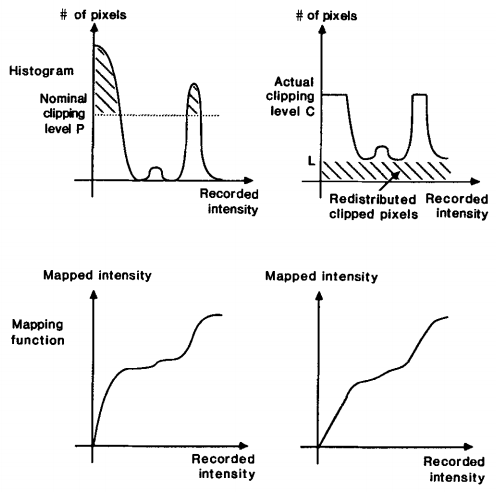
\includegraphics[width=0.7\textwidth]{images/clahe}
\caption[Visualizatoin of CLAHE algorithm]{Desription of CLAHE algorithm. Taken from Pizer, Zuiderfeld et al, 1987 \cite{pizer1987adaptive}  Note the  smoothen intensity CDF function (lower part of the figure) after reassigning some pixels with pixel values above the clipping value.}
\label{fig:clahe}
\end{figure}

%TODO improve image
\begin{figure}[H]
\centering
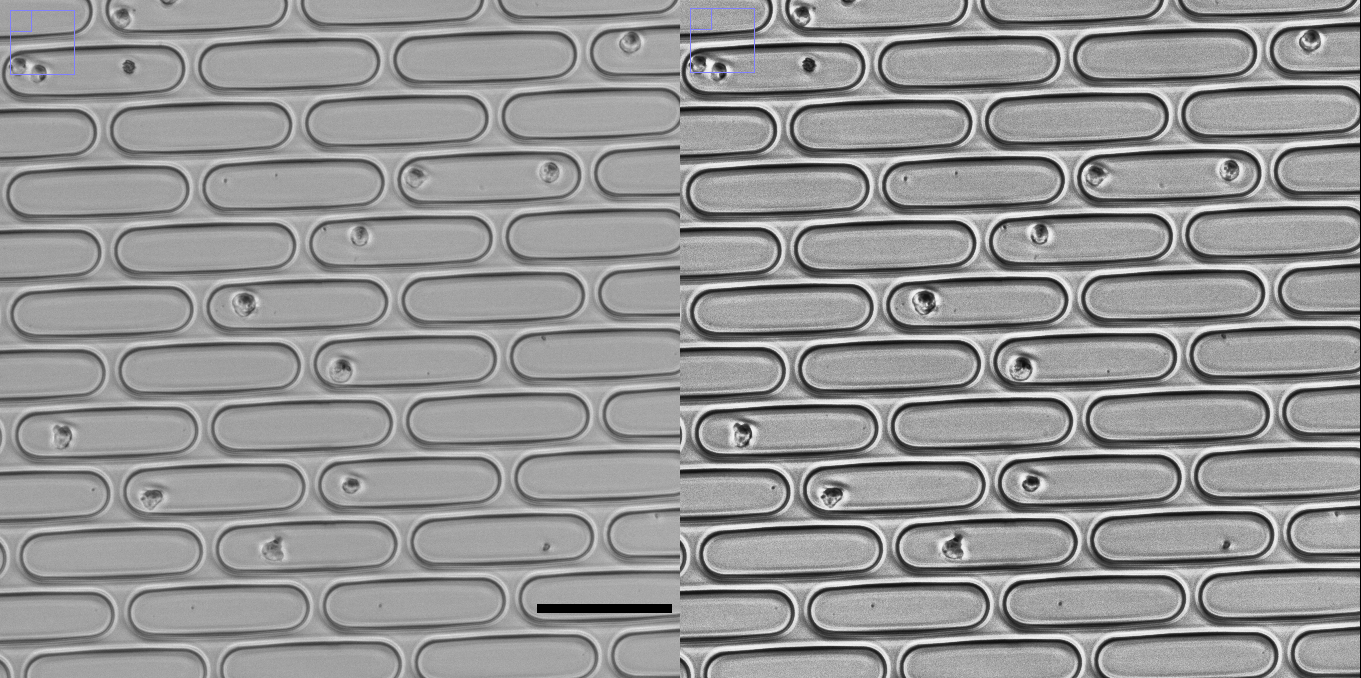
\includegraphics[width=\textwidth]{images/clahe_before_after}
\caption[Example of application of CLAHE algorithm]{The upper left corner of the in-focus brightfield chanenl of the image position 43 at time $t=0$: before (left) and after (right) the application of CLAHE on the image. Scale bar on the left figure is $100 \mu M$ long.}
\label{fig:clahe_before_after}
\end{figure}

\subsection{Subtraction by pixel-wise mean intensity}
\label{subsection:substraction_by_mean}

To substract an RGB image at time $M_t$ by its pixel-wise mean intensity $\langle M \rangle$, the average intensity for each pixel across all time points is made for a pixel. For a stack with $n$ images, we can simply define the pixel-wise mean of the R channel for pixel $(x, y)$ as following:

\begin{equation}
\langle M \rangle_{x, y, R} := \frac{\sum_{1 \leq t \leq n} M_{t, x, y, R}}{n}
\label{eq:mean_calc_rgb}
\end{equation}

The same applies to $\langle M \rangle_{x, y, G}$ and $\langle M \rangle_{x, y, B}$. For a grayscale stack we define analogously:

\begin{equation}
\langle G \rangle_{x, y} := \frac{\sum_{1 \leq t \leq n} G_{t, x, y, i}}{n}
\label{eq:mean_calc_gs}
\end{equation}

The pixel-wise substracted value of R channel is thus defined as point-wise operation for each pixel,

\begin{equation}
M^m_{t, x, y, R} := M_{t, x, y, R} - \langle M \rangle_{x, y, R}
\label{eq:mean_corr_rgb}
\end{equation}

The same applies to $\langle M \rangle_{x, y, G}$ and $\langle M \rangle_{x, y, B}$. The transformed RGB value is thus defined as

\begin{equation}
M^m_{t, x, y} := [M^m_{t, x, y, 1}; M^m_{t, x, y, 2}; M^m_{t, x, y, 3}
\end{equation}

As for a grayscale image we define following:

\begin{equation}
G^m_{t, x, y} := G_{t, x, y} - \langle G \rangle_{x, y}
\label{eq:mean_corr_gs}
\end{equation}

In the context of the single-cell enclosure on a wafer, this means that in the parts of images in which only dynamic movement of cells are observed, the pixel-wise mean intensity value of dynamic parts will be very low. Subtracting every pixel the area from every time point with the average will barely affect the original intensity value. On the other hand, applying the method on areas with static objects such as micro-trench wall and its surrounding reduces each pixel of the area with exactly the same intensity value as it barely changes during the experiment. This will nullify the static parts to large extent.

This method can be improved by iteratively repeating the calculation of $\langle M \rangle$. This will remove periodically static parts or static parts that abruptly moved (due to sudden shift in the well with regard to the camera for example). We call this algorithm \textbf{k-substraction by pixel-mean intensity}:

\begin{algorithm}[H]
 \KwData{$M_t$}
 \KwResult{$M^m_t$}
 \Parameter{$k$}
 \For{\forcond}{
 	calculates $\langle M \rangle$ from $M_t$ \;
 	$M^m_t = M_t - \langle M \rangle$ \;
 	$M_t = M^m_t$ \; 
 }
 \KwOut{$M_t$}
\caption{The k-substraction by pixel-mean intensity algorithm}
\label{algorithm:k_mean_substraction}
\end{algorithm}

\subsection{Cell recognition}
\label{subsection:cell_recognition}

Due to the cells' rotund shape, the \textbf{blob detection} family of algorithm is well-suited for recognizing cells. In our pipeline, we use the Laplacian of Gaussian (LoG) detector method.

\subsubsection*{Laplacian of Gaussian (LoG) detector}

Laplacian of Gaussian (LoG), also known as Marr-Hildreth-Opreator \cite{marr1980theory}, is among the first and still the most popular method for detecting blob \cite{sonka2014image}. It is characterized by applying the second derivative of the $\sigma$-scaled Gaussian to detect a blob in an image.

To derive the method we first consider a 2-dimensional Gaussian kernel function:

\begin{equation}
G(x,y) = \frac{1}{{2\pi \sigma^2}} e^{-\frac{x^2 + y^2}{2 \sigma^2}}
\label{equation:gauss_2d_log}
\end{equation}

As the name suggests, the representation of LoG operator is obtained by applying the Laplace-Operator $\Delta$ on the Gaussian,

$$
L(x, y) = \Delta G(x, y)
$$

This can be expanded into,

\begin{equation*}
\begin{aligned}
L(x, y) & = \frac{\partial^2 G(x, y)}{\partial x^2} + \frac{\partial^2 G(x, y)}{\partial y^2} \\ 
L(x, y) & = - \frac{1}{\pi \sigma^4} e^{-\frac{x^2 + y^2}{2\sigma^2}} \left( 1 - \frac{x^2 + y^2}{2 \sigma^2}\right)
\end{aligned}
\label{eq:svm_hard_margin}
\end{equation*}

Figure \ref{fig:pixdiff} shows the representation of the LoG operator in 2D. Notice the inverse hat characteristic giving it the nickname \textbf{Mexican hat operator}.

\begin{figure}[H]
\centering
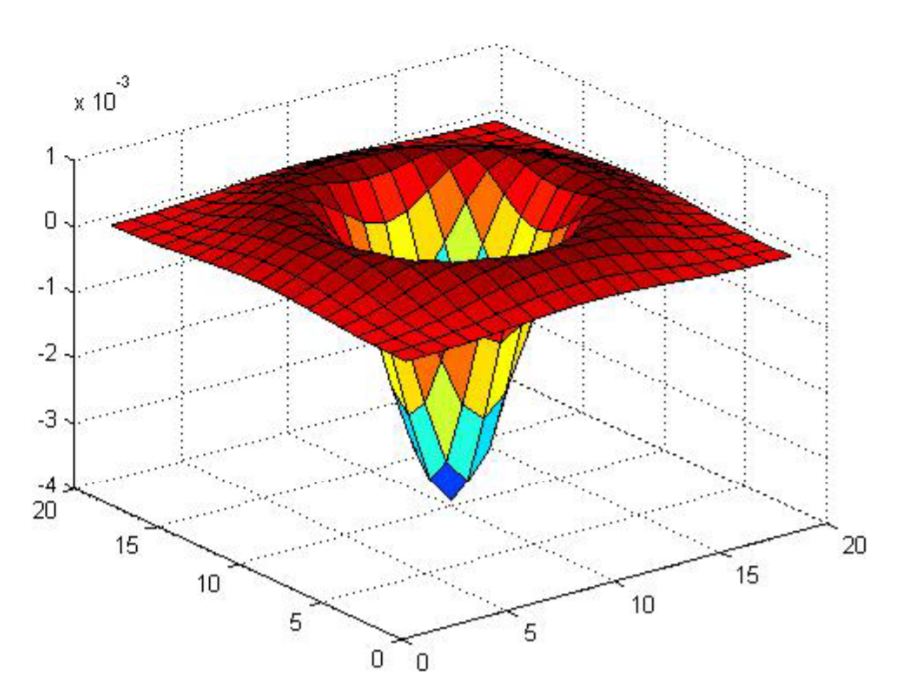
\includegraphics[width=0.6\textwidth]{images/log_operator}
\caption{A LoG operator. Notice the lack of dimension in an operator as it transforms an image (in one space) into another image (still in the same space).}
\label{fig:log_operator}
\end{figure}

The operator is then applied on two dimensional matrix of a grayscale image. To get maximum response from a blob, the zeros of the operator have to be aligned with the circle to be detected \cite{marr1980theory}. Figure \ref{fig:log_example} shows an example of idealized circle with the diameter $r$ and the corresponding response from the LoG operator on the surface of the circle. Applied to pre-processed out-of-focus image, LoG will return response with maxima in the center of cell sizes in similar fashion to the idealized circle.

\begin{figure}[H]
\centering
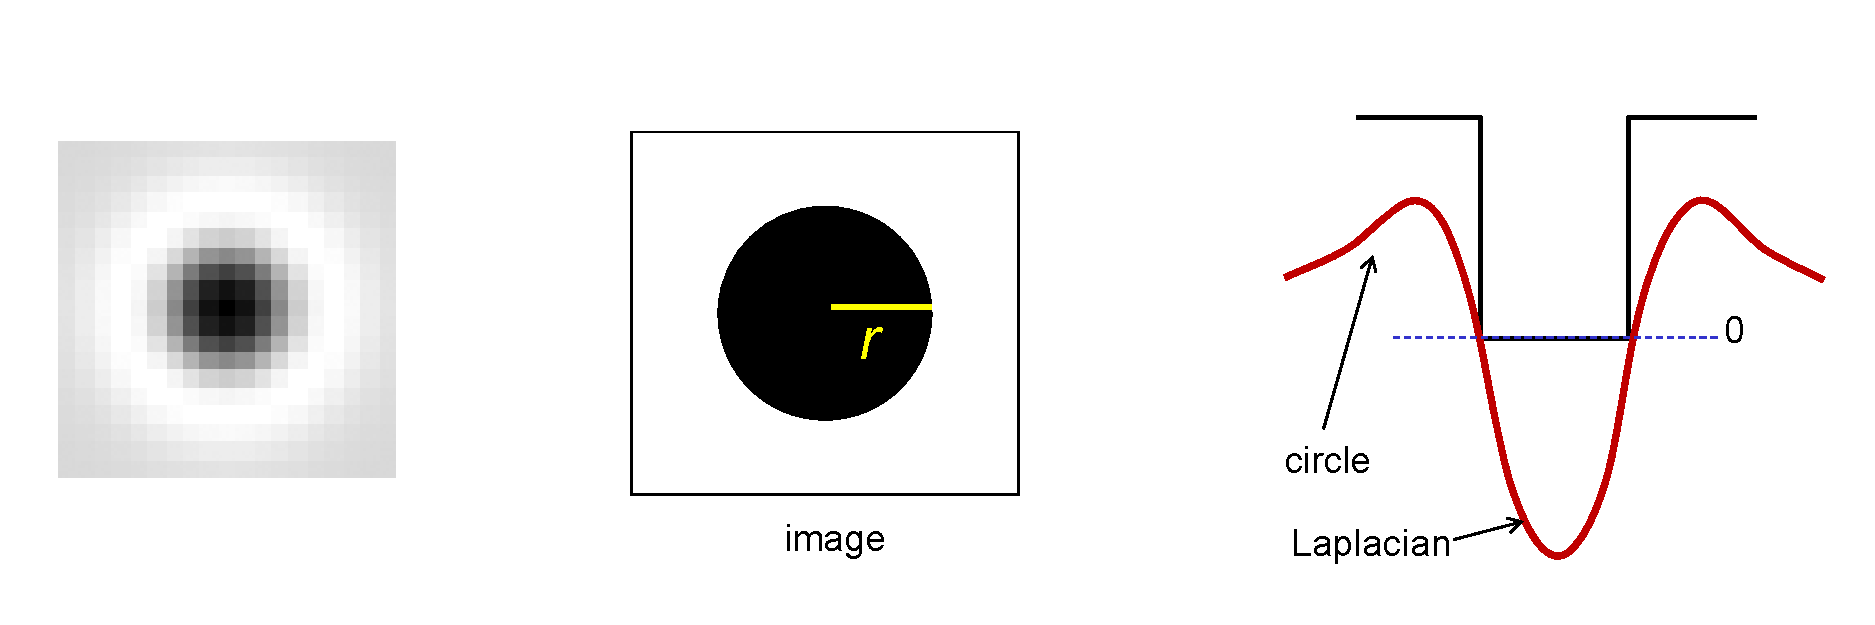
\includegraphics[width=\textwidth]{images/log_operator_example}
\caption[Example of application of the LoG operator]{Example of applying the LoG operator on a 2D circle. The minimum will be achieved if the diameter of the LoG operator is roughly equal to the diameter of the cell. This however does not to be the case. In case of non-perfect blob or blob with different diameter, local minimum can still be detected by the cell recognition algorithm \cite{tinevez2017trackmate}.}
\label{fig:log_example}
\end{figure}

\subsection{Cell tracking}
\label{subsection:cell_tracking}


To track detected cells, the Linear Assignment Problem (LAP) tracker, by Jaqaman et al, 2018, is used. The method builds upon the cell recognition method explained in Subsection \ref{subsection:cell_recognition}.

\subsubsection*{Linear Assignment Problem (LAP) framework of cell tracking}

The algorithm follows closely the case of linear assignment problem in bipartite graph. Given a bipartite graph $\mathcal{G}_b:= \{\mathcal{G}_1, \mathcal{G}_2\}$ and the assignment cost function 
$c(v_i, v_j)$ for $v_i \in \mathcal{G}_1$ and $v_i \in \mathcal{G}_2$, find a bijection $f_{\mathcal{G}_b} : \mathcal{G}_1 \rightarrow \mathcal{G}_2$ so that the total cost function:

\begin{equation}
\sum_{v_i \in \mathcal{G}_1} c(v_i, f_{\mathcal{G}_b}(v_i))
\label{eq:lap_standard}
\end{equation}


is minimized. As seen in Equation \ref{eq:lap_standard}, the cost function and its corresponding constraint (bipartite assignment) is linear. Hence, the "linear" part of the assignment problem.

We can frame our cell tracking problem as a variant of linear assignment problem. Recall that, for each slice, a set of blobs representing cells are detected. To track cells, each blob in a slice has to be connected with a blob in proceeding and succeeding slices (except in the case where a cell died).

Revisiting Subsection \ref{subsection:cell_recognition}, it is obvious that upon cell detection the next step is to track single cell movements in a stack is to assign detected blobs $\mathcal{G}_t$ at time $t$ with the blobs $\mathcal{G}_{t + 1}$ detected at time $t + 1$,  for $t \in [1:n - 1]$. To do that, first we define particle-to-particle cost function $c$. Jaqaman and his colleagues argued that \cite{jaqaman2008robust}, due to Brownian nature of cell movement, the square distance of blobs or its derivation should be used as cost function: 

\begin{equation}
d(v_i, v_j) = \| v_i - v_j\|^2_2
\label{eq:particle_cost_function}
\end{equation}

The algorithm is roughly divided into two main steps:

\begin{itemize}
\item  Creation of track segments through frame-to-frame blobs linking.
\item  Gap closing and cell division inference to achieve the closing of the track segments.
\end{itemize}

Both steps are framed as a linear assigned problem. In the first step, two consecutive slices $M_i$  and $M_{i+1}$ are optimized for the links. To do that, a $(m + n) \times (n + m)$ matrix $\mathcal{C}$ is created, where $m$ and $n$ refer to the number of detected blobs in $M_t$ and $M_{t + 1}$ respectively. The matrix contains four quadrants:

\begin{itemize}
\item The upper left quadrant ($m \times n$ elements) contains the costs of linking blobs in $M_t$ to those in $M_{t + 1}$, also known as the segment linking cost.
\item The upper right quadrant ($m \times m$ elements) contains the costs of not linking blobs in $M_t$ to any blobs in $M_{t + 1}$, also known as the segment stop cost.
\item The lower left quadrant ($n \times n$ elements) contains the costs of of not linking blobs in $M_{t + 1}$ to any blobs in $M_t$, also known as the segment start cost.
\item The lower right quadrant ($n \times m$ elements) is the auxiliary matrix used by the LAP framework as formalism for its algorithm. The matrix is created by transposing the upper right left quadrant and replacing all non-infinity cost with the minimal cost (by default 0).
\end{itemize}

The segment linking cost (upper left quadrant) is calculated as following:

\begin{gather*}
c(v_k, v_l) =
\begin{cases}
  (d(v_k, v_l) \cdot \left(1 + \sum_{\mathbb{f}} \left(3 W_{\mathbb{f}} \frac{ f_{\mathbb{f}1} - f_{\mathbb{f}2} }{f_{\mathbb{f}1} + f_{\mathbb{f}2}} \right)\right)^2 & \text{if } d(v_k, v_l) \leq d_{max} \\    
  \infty & \text{else}  
\end{cases}
\end{gather*}

where $\mathbb{f}$ refers to each feature penalty defined for the optimization and $W_{\mathbb{f}}$, $f_{\mathbb{f}1}$ and $f_{\mathbb{f}2}$ refer to the feature penalty factor, the value of feature $\mathbb{f}$ of $v_k$ and the value of feature feature $\mathbb{f}$ of $v_l$ respectively. Generally, only blob related features are used in the algorithm, e.g. total blob intensity, average blob intensity and minimum/maximum blob intensity. Note that:

\begin{itemize}
\item If the distance is larger than the pre-defined maximum distance $d_{max}$, then the link is forbidden. A blocking cost ($\infty$) is assigned between two blobs.
\item If no penalty feature is introduced then the cost is simply the squared distance of two blobs.
\end{itemize}

The non-linking cost (the upper right and lower left quadrants) is calculated as follows:

\begin{gather*}
c(v_k, v_l) =
\begin{cases}
  1.05 \cdot \mathbb{C} & \text{if } v_k = v_l \\
  \infty & \text{else}  
\end{cases}
\end{gather*}

where $\mathbb{C}$ is the maximum value of the upper left quadrant of the matrix.

The optimization over the matrix is then solved with the Munkers \& Kuhn algorithm \cite{munkres1957algorithms}, which solves the problem in cubic time $\mathcal{O}(n^3)$. The algorithm returns assignment minimizing the sum of the assignment costs.

The interpretation of the cost functions is following: without any penalty, the optimization problem favors the solution which minimizes the sum of squared distance between two blobs. This is in line with previously mentioned assumption of the Brownian motion of cells. By adding feature penalties, we aim at favoring linking blobs that are more similar to each other. In brute single particle linking problems, spots are generally all the same, and they only differ by the coordinate. However, there is a variety of problems for which these feature penalties can add robustness to the tracking process. In our case for example, the cells might pose several features that change over time depending on the treatment and cell-dependent characteristics (the phenomenon we further investigate using machine learning methods, see Subsections \ref{subsection:svm} and \ref{subsection:rf} and Section \ref{section:ml_results}).

%TODO decide whether Random Forest should be added

Upon the linking of blobs into track segments, more refinement is then done to achieve globally optimal cell tracks configuration. To do this, three events are considered in our model:

\begin{itemize}
\item In case of \textit{gap closing} events, the end of a track segment is linked to the start of another track segment.
\item In case of \textit{splitting} events, the stat of one track segment is linked to non-terminal part of another track segment.
\end{itemize}

The matrix is created in similar fashion to the cost matrix in the first step, with the details best referenced directly to the article by Jaqaman et al \cite{jaqaman2008robust}. Also similar to the first part is the use of penalty features during segment creation. Unlike the the first part however, the segment merging cost is blocking ($\infty$) if the segments in question are separated by frames larger than pre-defined maximum number of frame gaps.

The optimal solution for the problem is again found using the Munkers \& Kuhn algorithm \cite{munkres1957algorithms}.

\subsection{Shift correction}
\label{subsection:shift_correction}

Shift correction is done to correct the slice alignment within stacks. As mentioned in Subsection \ref{subsection:exp_setup}, the images were captured discretely at the frequency of $\frac{1}{10 min}$ and $\frac{1}{30 min}$ depending on the channel. During this time, the setup might move albeit very slightly causing very small shift. The bulk of the shift, however, happened during the introduction of the  drug treatment. At this time, the drug is introduced to the medium using a pipette. The liquid released pushes the wafer somewhat causing noticable shift in camera's field of view (see Table \ref{table:inferred_shift} of Appendix \ref{chapter:appendix_tables} for the inferred shift in every image position).

Now, consider the case in which the images are shifted in a time-lapsed movie during the introduction of drug treatment. No rotation of camera is assumed, hence there are only two degree of freedoms (vertical and horizontal). Thus, a shift can be defined as a vector movement $\vec{v}$ of all points $x_{i,j} \in M_t$ in the time-lapse from time $t$ to $t + 1$. Given two degrees of freedom and discreteness of the problem due to pixel representation, the task is reduced to finding difference in x- and y-axis ($\delta_x$ and $\delta_y$), so that the difference of transformed pixels at $t$ and $t_{i+1}$ are minimized, i.e.:

$$
arg\,min_{\delta_x, \delta_y} \{d(M_{t}, M_{t + 1}^{\delta_x, \delta_y}\}
$$

Where $M_{t + 1}^{\delta_x, \delta_y}$ is the entries of matrix $M_{t + 1}$ after applying the shift $\vec{v} := (\delta_x, \delta_y)^T$, i.e.

$$M_{t + 1, \, x, \, y}^{\delta_x, \delta_y} = M_{t + 1, \, x - \delta_x, \, y - \delta_y}$$

and the distance function $d$ is defined as all-channel all-pixel sum of differences between two image:

$$
d_{RGB}(M_i, M_j) = \sum_{c \, \in \, \{R, B, G\}} \sum_{x} \sum_{y} \vert M_{i, x, y, c} - M_{j, x, y, c} \vert
$$

Since some pixels are lost from the field of view during a shift, only a subset of subsequent images is used to determine the shift, preferably those around the center point. This will allow the largest search space possible, since the distance to all four margins of the image is maximized at the center point. The search for the optimal $(\delta_x, \delta_y)$ pair is implemented as a grid search along the x- and y-axis. An example of the search grid is shown in Figure \ref{fig:searchgrid}. Algorithm \ref{algorithm:shift_inference_rgb} shows the pseudocode of shift inference algorithm for RGB images.

\vspace{10mm}

\begin{algorithm}[H]
 \KwData{$M_t$, $M_{t + 1}$}
 \KwResult{$M^m_t$}
 \Parameter{$d, l$}
 $D$ distance matrix for various shifting configurations \;
 $c := (c_x, c_y)$ coordinate of center pixel of $M_t$ \;
 $M'_t  := M_{t}[c_x - l:c_x +l][c_y - l:c_y +l]$ sub-image of $M_t$ centered around $(c_x, x_y)$\;
 \For{$i=-d$ \KwTo $d$}{
 	\For{$j=-d$ \KwTo $d$}{
 		$c' := (c_y - i, c_y - j)$ \;
 		$M'_{t + 1} := M_{t + 1}[c'_x - l:c'_x +l][c'_y - l:c'_y +l]$\;
 		$D[i,j] := d_{RGB}(M'_t, M'_{t + 1})$
 	}
 }
 \KwOut{$arg\,min_{i, j} \{D\}$}
 \vline
\caption{Shift inference algorithm for RGB images}
\label{algorithm:shift_inference_rgb}
\end{algorithm}

\vspace{10mm}

Since the time-lapsed data consists mainly of grayscale image, the RGB encoding could be the directly transformed to grayscale encoding (see Equation \ref{equation:rgb_to_gray_def} of Subsection \ref{subsection:image_encoding}). Using the transformed method also speeds up the calculation process since the distance function only computes the difference of grayscale channel's values:

$$
d_G(G_i, G_j) =  \sum_{x} \sum_{y} \vert G_{i, x, y} - G_{j, x, y}\vert
$$

For this case, the shift inference algorithm can simply be modified by replacing $d_{RGB}$ with $d_G$.

Due to lost pixels around the margin of before and after images, only the overlapping part of both slides are included after the correction. Thus, for an inferred shift of $(\delta_x, \delta_y)$, the new dimension of the images is then $(m - \delta_x) \times (n - \delta_y)$. This change would then propagation to the other time-lapse images to maintain consistency of the images.

Ideally, the shift correction should be done for each time point to reduce the track dropout rate caused by image shifts. This is however computationally very expensive. Moreover, inferring the shift for every recording time is not really necessary since the biggest shift, as mentioned before, only happens right before and after the treatment. The difference diference between consecutive images of the image position 26 can be seen in \ref{fig:pixdiff}. Here we can see that the major spike of difference is only observed upon the introduction of the drug treatment.

As described in Subsection \ref{subsection:cell_tracking}, the tracking algorithm allows certain amount of tolerance represented as maximum distance $d_{max}$. In this regard, the frame shifts happening not during the drug treatment introduction are way within the tolerance of our tracking algorithm. As shown in (TODO: add droput rate figure), the dropouts caused by frame shifts in the other time points are basically noisy dropout caused by random noises in the time-lapse movie being tracked as cells \cite{jaqaman2008robust}.

\begin{figure}[H]
\centering
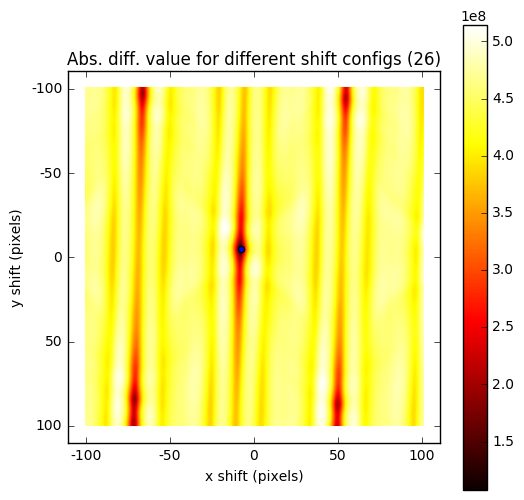
\includegraphics[width=0.6\textwidth]{images/search_grid}
\caption[Example of search grid from the shift inference algorithm]{Search grid shift for the image position 26. The search was conducted for shift between the last time point before and the first time point after the drug treatment. The minimum is marked with thick black dot, which is returned after every grid-search call as inferred shift. In the position, the shift was inferred to be 8 pixels upwards and 5 pixels leftwards. Note the repeating pattern of relatively favorable configurations after approximately 50 horizontal and 100 vertical pixels caused by lattice nature of the micro-trenches.}
\label{fig:searchgrid}
\end{figure}

\begin{figure}[H]
\centering
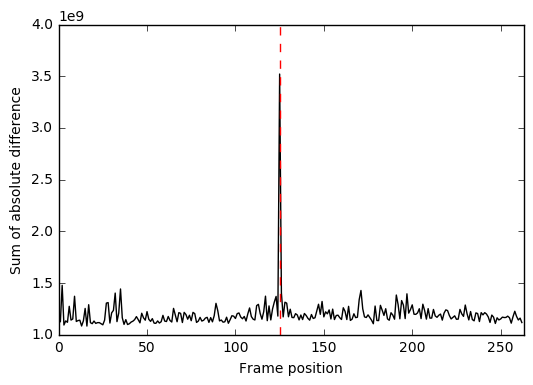
\includegraphics[width=0.8\textwidth]{images/pixdiff}
\caption[Slice-wise sum of pixel difference in a stack]{Pixel difference between consecutive frames in the image position 26. In most cases, the pixel difference between the frames is mainly caused by moving cells. The difference during the introduction of the drug treatment (red dashed line), on the other hand, is caused by physical shift of the frame. While moving cells mostly caused minimum noise-like pixel difference, the physical shift of field of view distorts the physical alignment and evokes immense pixel difference.}
\label{fig:pixdiff}
\end{figure}

\subsection{Support vector machine (SVM)}
\label{subsection:svm}

In machine learning, an SVM is a construct which, given the training set $\mathbf{S} \subset \mathbf{D}$ with,

$$
\mathbf{S} = \{\mathbf{x_1}, \cdots, \mathbf{x}_{ \vert \mathbf{S} \vert }\}
$$

and corresponding target class,

$$
\mathbf{T} = \{y_1, \cdots, y_{\vert \mathbf{S} \vert}\}
$$

finds following things,

\begin{itemize}
\item A hyperplane that separates the input by its class, so that every point belonging to one class is located on one side of the hyperplane. This hyperplane is, in turn, defined by,
\item support vectors.
\end{itemize}

A hyperplane is defined as a set of points $\mathbf{x}$ in $\mathbf{S}$ satisfying following criteria,

\begin{equation}
\mathbf{w} \cdot \mathbf{x} - b = 0
\label{equation:hyperplane}
\end{equation}

(See Figure \ref{fig:svm}) where $\mathbf{w}$ and $\frac{b}{\| \mathbf{w} \|}$ denote the normal vector to the hyperplane and the distance of the hyperplane from the origin along the normal vector $\mathbf{w}$. For every class $c_i$, the set of of data points satisfyling criteria,

\begin{equation}
\mathbf{w} \cdot \mathbf{x} - b = c_i
\label{equation:support_vector}
\end{equation}

are called support vectors. The distance from the hyperplane to support vectors is thus,

$$\frac{1}{\| \mathbf{w} \|}$$

For two-classes classification, the classes are conventionally annotated as $-1$ and $1$. As the Equations \label{equation:support_vector} suggests, for every point beyond (seen from the perspective of hyperplane) the support vectors of the class $c = -1$, following unequality applies,

\begin{equation}
\mathbf{w} \cdot \mathbf{x} - b < -1
\label{equation:svm_class_1}
\end{equation}

The analogous applies to the class $c = 1$,

\begin{equation}
\mathbf{w} \cdot \mathbf{x} - b > 1
\label{equation:svm_class_2}
\end{equation}

\begin{figure}[H]
\centering
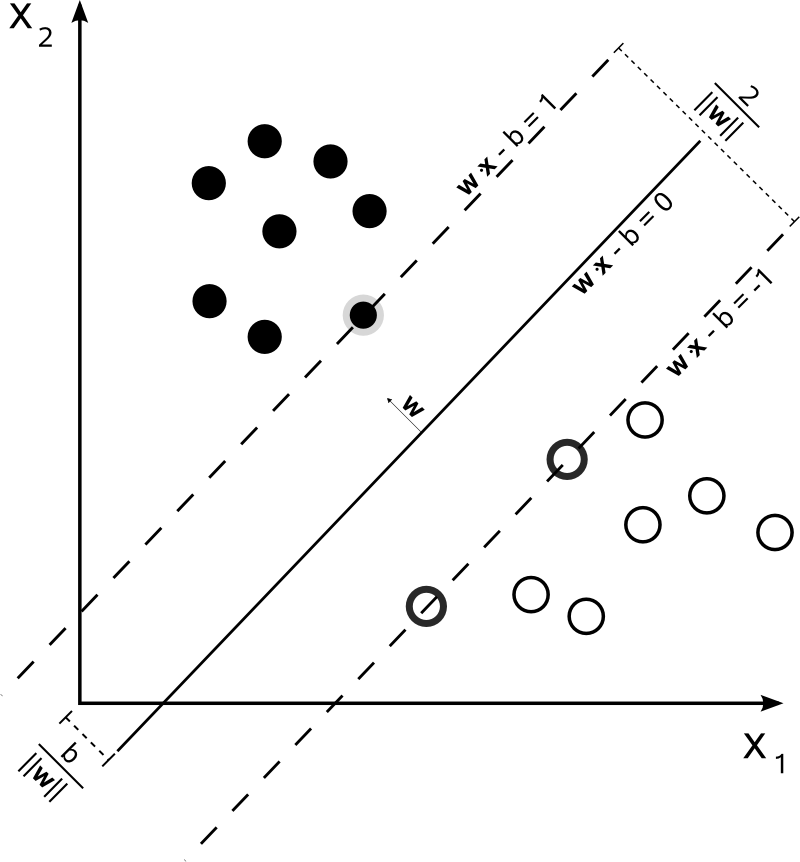
\includegraphics[width=0.5\textwidth]{images/svm}
\caption[Illustration of SVM in 2D]{Illustration of a support vector machine in 2D. For black class there is one hyperplane-definining point (marked with grey margin) while for white class there are two (marked with bold black margin). The support vector $\mathbf{w}$ is maximized for each class.}
\label{fig:svm}
\end{figure}

Following large margin principle \cite{vapnik1964note, murphy2012machine}, an SVM tries to find support vectors that maximize $\| \mathbf{w} \|$. Given separability of the training data, the support vector $\mathbf{w}$ can then be solved by solving following optimizing problem, 

\begin{equation*}
\begin{aligned}
& \underset{\mathbf{
w}}{\text{minimize}}
& & \| \mathbf{w}\| \\
& \text{subject to}
& & y_i(\mathbf{w} \cdot \mathbf{x}_i - b \leq 1) \text{ for } i = 1, \cdots \| \mathbf{S} \|.
\end{aligned}
\label{eq:svm_hard_margin}
\end{equation*}

This hard-margin only converges only when the data are linearly separable in mapped space (also known as \textbf{feature space}). This is especially bad since many problems are not linearly separable in their original space. There are two fundamentals way of relaxing this problem to enable classification using SVM:

\begin{itemize}
\item Relaxation of the definition of the SVM by allowing data points to be misclassified.
\item Blowing up the input space into sufficiently high dimensional features using the kernel trick.
\end{itemize}

\subsubsection*{Relaxation of SVM}

A relaxation of above explained problem is known as soft margin SVM or $\xi$-SVM \cite{cortes1995support}. The problem allows misclassification of some training data. In SVM, misclassification occurs when a data point belonging to a certain class $c_j$ is located \textbf{not} in the area defined by the margin $\mathbf{w} x_{c_j} = c_j$ for class $c_j$.

The problem is thus reduced to minimizing following term,

\begin{equation}
\left[\frac{1}{n} \sum_{i=1}^{\vert \mathbf{S} \vert} \max\left(0, 1 - y_i(\mathbf{w} \cdot \mathbf{x_i} - b)\right) \right] + \lambda\| w \|^2
\label{eq:soft_margin_svm_term}
\end{equation}

The term inside of summation is called \textbf{classification error}. For correctly classified class we have $\mathbf{w} \cdot \mathbf{x}_i - b \leq -1$ and $\mathbf{w} \cdot \mathbf{x}_i - b \geq 1$ for $c_i = -1$ and $c_i = 1$ respectively, i.e. the summation term is $0$ for every correctly classified data point. The coefficient $\lambda$ is regularization coefficient which penalizes the magnitude of normal vector $\mathbf{w}$. Note that the higher the dimension of $\mathbf{w}$ the larger the penalty is. This is important for next part on \textbf{kernel methods}.

Minimizing Term \ref{eq:soft_margin_svm_term} is equal to optimizable with differentiable objective function \cite{nocedal2006numerical}. We can for example introduce a variable $\zeta_i$ defined as,

\begin{equation}
\zeta_i = \max(0, 1 - y_i(\mathbf{w} \cdot \mathbf{x}_i - b))
\label{eq:svm_zeta}
\end{equation}

This can be written as $y_i(\mathbf{w} \cdot \mathbf{x}_i - b) \geq 1 - \zeta_i$. Geometrically this is the maximum distance of a wrongly classified data point from the support vector. Using Definition \ref{eq:svm_zeta} we can reduce optimization posed in Term \ref{eq:soft_margin_svm_term} to,

\begin{equation*}
\begin{aligned}
& \underset{\mathbf{
w}}{\text{minimize}}
& & \frac{1}{\vert \mathbf{S} \vert} \sum_{i=1}^{\vert \mathbf{S} \vert} \zeta_i + \lambda \| \mathbf{w} \|^2 \\
& \text{subject to}
& & y_i (\mathbf{w} \cdot \mathbf{x}_i - b) \leq 1 - \zeta_i \\
& \text{and} && \zeta_i \geq 0 \text{ for all } i.
\end{aligned}
\end{equation*}

\subsubsection*{Kernel method}

As mentioned before, the optimization problem posed in Subsection \ref{eq:svm_hard_margin} converges only in the case of linear separability of training data. While this mostly is not the case, Vapnik and Cortes \cite{cortes1995support} proposed the so-called \textbf{kernel trick}. It utilizes a kernel function $\Phi$ which maps the training set into high dimensional space representation. Essentially, a kernel function $\Phi: \mathbb{R} \times \mathbb{R} \rightarrow \mathbb{R}^+$ is a symmetric and non-negative function following the criteria by Mercer \cite{mercer1909functions} defining it as, among others, general measure of similarity between two vectors.

In our case, we focus on two very well-known examples of kernel function, \textbf{the polynomial kernel function of order n}, defined as,

\begin{equation}
\Phi_{RBF}(\mathbf{x}_i, \mathbf{x}_j) = \left(\mathbf{x}_i^T \mathbf{x}_j + r \right)^n \text{ with } r > 0
\label{eq:svm_rbf}
\end{equation} 

and the \textbf{radial basis function (RBF)}, defined as,

\begin{equation}
\Phi_{RBF}(\mathbf{x}_i, \mathbf{x}_j) = exp\left(\frac{\| \mathbf{x}_i - \mathbf{x}_j \|^2}{2 \sigma^2}\right)
\label{eq:svm_rbf}
\end{equation}

In both examples we can observe the assumed dimensionality of target feature space. A polynomial kernel function of order n maps the training data to $n$-dimensional feature  space. Thus, blowing up the training data into higher dimensional requires the explicit assignment of a very high $n$ value. The  radial basis function on the other hand does not assume any dimensionality (or rather, it assumes unbounded dimensionality) as the Gaussian function used only assumes the input vectors $\mathbf{x}_i$ and $\mathbf{x}_j$ to be of the same dimensionality. 

While assuming very high/unbounded dimensionality seems convenient at the start, this is not very straightforward, since:

\begin{itemize}
\item Given a non-powerful kernel function $\Phi$ that only maps the input into bounded number of dimension, the optimization problem may not converge if there is no representation that is mapable  using the kernel function.
\item Given a powerful kernel function $\Phi$ capable of blowing up the dimension to very high dimensions kernel might settle for an unnecessarily sparse dimensional reducing the generalizability of the problem.
\end{itemize}

\subsubsection*{Regularization}

One solution is too introduce regularization. As already shown in Term \ref{eq:soft_margin_svm_term}, we can add a regularization term such as, 

\begin{itemize}
\item $L_1$-regularization: $\lambda \| \mathbf{w} \|^2$ \cite{park2007l1}, and
\item $L_2$-regularization (Tikhonov regularization): $\lambda \| \mathbf{w} \|$ \cite{tikhonov1977solutions}.
\end{itemize}

Adding regularization will control against overfitted model by penalizing higher dimensional hyperplane $\mathbf{w}$ as it the error will get blown up the higher dimensional, and its error minimizing hyperplane, are chosen.

\subsubsection*{Regressive SVM}

SVM can be extended to enable regression. The method, initially proposed by Smola, Vapnik et al \cite{drucker1997support} and commonly known as Support Vector Regression (SVR), modifies the optimization problem of standard SVM to:

\begin{equation*}
\begin{aligned}
& \underset{\mathbf{
w}}{\text{minimize}}
& & \frac{1}{2} \| \mathbf{w} \| \\
& \text{subject to}
& & y_i - \langle \mathbf{w} , \mathbf{x}_i \rangle - \mathbf{b} \leq \epsilon \\
& \text{and} && \langle \mathbf{w} , \mathbf{x}_i\rangle + \mathbf{b} - \mathbf{y}_i \leq \epsilon \\
\end{aligned}
\end{equation*}

where $\mathbf{b}$ and $\langle \bullet , \bullet \rangle$ refer to the intercept of a linear model and  the inner product operator. Note the term

$$
\mathbf{y} = \langle \mathbf{w} , \mathbf{x}_i \rangle + \mathbf{b} + \sigma
$$

being the term for standard linear model with intercept $\mathbf{b}$  and error term $\sigma$.

%\subsection{Random Forests (RF)}
%\label{subsection:rf}

\subsection{Pearson's correlation coefficient (PCC)}

In statistics, the PCC is a measure of the linear correlation between two random variables $X$ and $Y$ \cite{fahrmeir2016statistik}. It has a value ranging from $-1$ to $1$. A correlation value of $-1$ denotes a perfectly inverse correlation, 0 denotes no linear correlation and $1$ denotes a perfect positive correlation.

For two random variables $X$ and $Y$, the PCC is defined as follows:

\begin{equation}
\rho_{X, Y} = \frac{\mathbf{cov}(X, Y)}{\sigma_X \sigma_Y}
\label{eq:rho}
\end{equation}

where $\mathbf{cov}(X, Y)$ is the covariance of random variables $X$  and $Y$, $\sigma_X$ is the standard deviation of $X$ and $\sigma_Y$ is the standard deviation of $Y$.

The covariance of two random variables is in turn defined as

\begin{equation}
\mathbf{cov}(X, Y) = E[(X - \mu_X)(Y - \mu_Y)]
\label{eq:cov}
\end{equation}

with $E[X]$ denoting expected value of a random variable $X$. Combining Equations \ref{eq:rho} and \ref{eq:cov} and using definition of mean ($\mu_X = E[X]$) and standard deviation ($\sigma^2_X = E[(X - E[X])^2]$) we can derive the formula of $\rho_{X,Y}$ to:

\begin{equation}
\rho_{X, Y} = \frac{E[XY] - E[X]E[Y]}{\sqrt{E[X^2] - [E[X]]^2} \sqrt{E[Y^2] - [E[Y]]^2}}
\label{eq:rho_cov}
\end{equation}

To calculate p-value, we  first calculate $t^*$-value, defined  as

\begin{equation}
t^* = \frac{\rho_{X,Y} \sqrt{n - 2}}{\sqrt{1 - \rho_{X,Y}^2}}
\end{equation}

where $n$ denotes the number of observation. The p-value is then defined as probability of Student's t distribution $T$ with $n - 2$ degrees of freedom having value $x$ smaller than $t$, i.e.

\begin{equation}
p = P(Z \leq t^* \mid Z \sim T)
\end{equation}

\subsection{F-Test}

In statistics, F-Test is statistical test in which the statistic $F_{X,Y} $ is assumed to be F-distributed under null Hypothesis, i.e. $F_{X,Y} \sim F(n_1, n_2) \mid  H_0$ \cite{fahrmeir2016statistik}. The distribution arise from the ratio of the $\chi$-squared variance of two normally distributed random variables, i.e. for two random variables $U \sim \chi^2(n_1)$  and $V \sim \chi^2(n_1)$, the ratio

\begin{equation}
F = \frac{U / n_1}{V / n_2}
\end{equation}

is then F-distributed. The symbols $n_1$ and $n_2$ denote the degree of freedom of $U$ and $V$. Conducting an F-test is thus reduced to checking whether, given two distributions $X$ and $Y$, the F statistic of two distributions is F distributed. To do that, we first compute the F statistic  of both distributions, 

\begin{equation}
F_{X,Y} = \frac{\mathbf{var}(X)}{\mathbf{var}(Y)}
\end{equation}

with $\mathbf{var}$ denoting the variance of the distribution $\mathbf{var}(X) = E[(X - \mu)^2]$
The degree of freedom of both distributions is defined as,

\begin{align}
  n_1 &= \vert X \vert - 1 \label{eq:ftest_dof_x} \\
  n_2 &= \vert Y \vert - 1\label{eq:ftest_dof_y}
\end{align}

The cumulative density function (cdf) $F_{cdf}$ of the F-distribution is given by

\begin{equation}
F_{cdf}(x; n_1, n_2)= \mathbf{I}_{\frac{n_1 x}{n_1 x + n_2}}\left (\tfrac{n_1}{2}, \tfrac{n_2}{2} \right)
\end{equation}

where $\mathbf{I}_x$ is the regularized beta function

\begin{equation}
\mathbf{I}_x(a,b) = \frac{\mathbf{B}(x;\,a,b)}{\mathbf{B}(a,b)}
\end{equation}

and $\mathbf{B}$ is the beta function

\begin{equation}
B(x;\,a,b) = \int_0^x t^{a-1}\,(1-t)^{b-1}\,dt.
\end{equation}

Using the  standard definition of one-sided right tail p-value we can derive for the p-value of the F statistic as following:

\begin{align}
  p_F &= Pr(Z \geq F_{X,Y} \mid H_0) \nonumber \\
  p_F &= 1 - F_{cdf}(F_{X,Y}; \, n_1, n_2)\label{eq:ftest_dof_y}
\end{align}

for $Z \sim F(n_1, n_2)$.

\chapter{Analytic Pipeline}

In this chapter the image and data analytic pipeline is presented. Each pipeline of image processing analysis is elaborated with reference to publications and the definitions from Chapter \ref{chapter:data_and_method}.
Every method developed/used in the pipeline is brought forward and explained with references to scientific literature and the definitions brought forward in Chapter \ref{chapter:data_and_method}.

\section{Image computing}

To assess single cell characteristics (like its lifetime, time-to-death, division time, daughter cells and other information relating to its time- and generation-dependent cell cycle information), we track all cells in the brightfield channel from the start of the movie, assign cells to individual micro-trenches to e.g. filter out micro-trenches with multiple starting cells, and determine cell death via marker onset in the fluorescent channels.

Figure \ref{fig:pipeline1}a shows how the image is sequentially processed from out-of-focus image to cell trees information.

\section{Micro-trench masking}
\label{subsection:micro_trench_masking}

Several techniques could be applied to highlight certain areas in the image. In Subsection \ref{subsection:cv_advances}, several advances in computer vision methods are described. Furthermore, general advances in the field of machine learning is chronicled in Subsection \ref{subsection:ml_advances}. While the collection of advanced methods for region and image detection abound \cite{krahenbuhl2011efficient, long2015fully, ronneberger2015u}, some simple interpretable methods could be used best to detect and mask the micro-trenches. In particular,  we can see that the area around a micro-trench exposes strong intensity gradient (see Figure \ref{fig:pos41_brightness}): the area around the margin of a micro-trench is much darker than the other parts of the well. This can be explained by the fact that the light is reflected less around the wall area and thus the intensity decreases. Additionally, the light beam coming out of the laser is not perfectly perpendicular to the well and thus the non-perpendicular reflection is not reflected back to the camera sensor.

Before us, there are several methods that exploit this kind of phenomenon. Cheng et al \cite{cheng2015global} for example shows it is possible to recognized salient objects in image by using contrast and brightness adjustment. Our method on the other hand, goes further by doing robustness improvement by doing noise cancellation step (See \ref{subsubsection:rats}).

\begin{figure}[H]
\centering

\begin{subfigure}{0.8\textwidth}
  \centering
  
\includegraphics[width=\textwidth]{images/pos_41_cut_highlight_y_500}
  \caption{}
  \label{fig:pos41_highlight}
\end{subfigure}%

\begin{subfigure}{\textwidth}
  \centering
  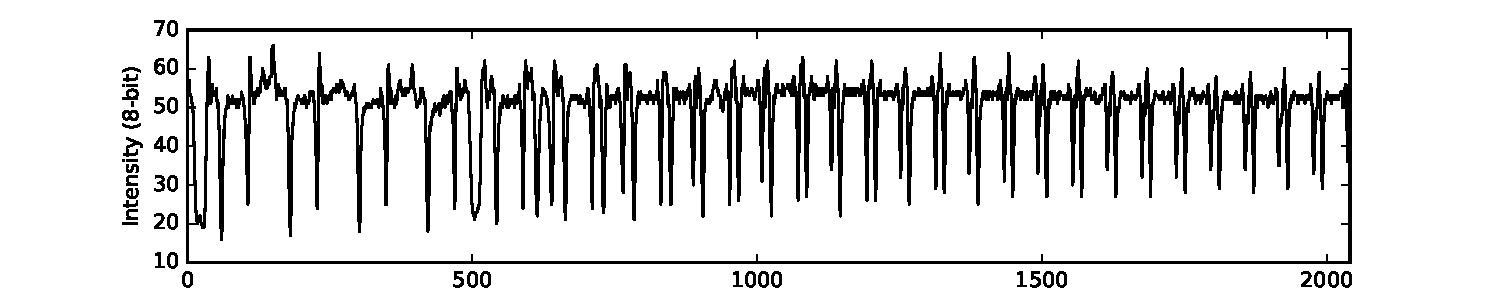
\includegraphics[width=\textwidth]{images/pos_41_cut_highlight_y_500_contrast}
  \caption{}
  \label{fig:pos41_contrast}
\end{subfigure}%
\caption[Example of intensity values along the vertical axis in an out-of-focus image]{(a) The highlighted area around the 500-th column of the first slice of the image position 41. The range starts from the 450-th until the 550-th column. (b) The intensity of the red-marked area in (a), the region around micro-trench margin is indicated by the sudden drop of intensity. Note also the slow drift of the intensity as the pixel goes south (right side of the plot). This phenomenon is called \textit{intensity gradient} (see Subsection \ref{subsection:gaussian_blur} for more.}
\label{fig:pos41_brightness}
\end{figure}

We could thus exploit this knowledge by designing micro-trench masking algorithm as follows:

\subsection{Brightness and contrast adjustment of in-focus image}
\label{subsubsection:brightness_contrast_adjustment}

First, we adjust the brightness and contrast so that the area far away from the margin is encoded as maximum intensity, while the area around the margin is encoded as minimum intensity. One simple and robust way to do this is to reduce the intensity of each position with the maximum intensity value of the region around the margin.

Mathematically, we can define two sets of points, $\mathfrak{M}$ and $\mathfrak{S}$. $\mathfrak{M}$ refers to the set of points around the trench margin while $\mathfrak{S}$ denotes the set of points far away from it. This brings us to the following transformation,

$$
J_i(i, j) := I_t(i, j) + argmax_{(x, y) \, \in \, \mathfrak{M}}{I_t(x, y)}
$$

creating transformed intensity $I^t$.

As can be seen in Figures \ref{fig:pos41_density} and \ref {fig:pos41_brightness}, while sets $\mathfrak{M}$ and $\mathfrak{S}$ are locally separable, across the board this does not seem so clear. We can thus improve the transformation by also adjusting the contrast parameter $\alpha$ by increasing it so that $\alpha > 1$. This brings the pixels with similar intensity values around the decision boundary (somewhere between the two distributions in Figure \ref{fig:pos41_density}) apart and thus ameliorates the determination of decision boundary by the user. Applying this, we have now the new transformation:

$$
J_i(i, j) := \alpha I_t(i, j) + argmax_{(x, y) \, \in \, \mathfrak{M}}{I_t(x, y)} \text{ with } \alpha > 1
$$

creating transformed intensity $I^t$.

Note that this is still not a perfect transformation, as there are some pixels in $\mathfrak{S}$ with intensity lower than the minimum intensity of pixels in $\mathfrak{M}$. Besides doing this manually, we also improve this by refining the transformed intensity $I^t$ further with the next step: Robust Automatic Threshold Selection.

Subfigures \ref{fig:pipeline1}j and \ref{fig:pipeline1}k show images of micro-trenches before and after brightness and contrast adjustment in the image processing pipeline.  The step is done manually for each image position using the \textbf{Bright/Contrast Adjustment} function in Fiji.

\subsection{RATS denoising}
\label{subsubsection:brightness_contrast_adjustment}

After brightness and contrast adjustment, some parts inside the micro-trench still have pixels  that were not transformed to complete white color (maximum intensity). This can be removed by the global and local noise correction through Robust Automatic Threshold Selection (RATS, see Subsection \ref{subsubsection:rats}). The algorithm is applied on each adjusted brightfield image, which creates a binary image of the micro-trench margins.

Subfigures \ref{fig:pipeline1}k and \ref{fig:pipeline1}l show the input and output of  RATS in the image processing pipeline. The noise partaining in a micro-trench is removed upon application of gradient-based filtering. We can thus say that,

\begin{itemize}
\item the first part of RATS ($\mathbb{g}$-filtering by $\lambda \sigma$) is designed to move global level noise  which in this case means white noises coming from non-perfect reflection of light from the well.
\item the second part of RATS (recursive $\mathbb{g}$-filtering by $T_r$)is designed to remove local noise cause by local distortion due to location-specific artifacts (direction of incoming light not perfectly perpendicular with regard to micro-trench's base etc).
\end{itemize}

The step is done automatically using the \textbf{Robust Automatic Threshold Selection (RATS)} plugin in Fiji with following parameters:

\begin{table}[H]
\centering
\begin{tabular}[t]{ l | c }
Parameter & Value \\
\hline
\texttt{noise\_threshold} & 25 \\
\texttt{lambda\_factor} & 3 \\
\texttt{min\_leaf\_size\_pixels} & 408 \\
\end{tabular}
\end{table}

\subsection{Micro-trench mask filling}

After applying brightness and contrast adjustment and RATS, the image now contains only the margin of micro-trenches. We can then fill these holes to create micro-trench masks. Subsection \ref{subsection:holes_filling} desribes the holes filling algorihm. The step is done automatically using the \textbf{Fill Holes} function in Fiji. Subfigures \ref{fig:pipeline1}l and \ref{fig:pipeline1}m show the input and output of the holes filing algorithm in the image processing pipeline. Upon holes filling, Each mask (appearing as a black rod-like form) is assigned a unique identity, which is then used as an identifier for tracks in both the brightfield and the fluorescent channel for filtering of cells and clones (see Sections \ref{section:pipeline_brightfield} and \ref{section:pipeline_fluoroscent}).

\section{Single cell tracking in the brightfield channel}
\label{section:pipeline_brightfield}

To identify and track single cells from movie start, each out-of-focus brightfield image is processed in the following way (see Figure \ref{fig:pipeline1}a for pipeline visualization): 

\subsection{Gaussian blurring}

First, a Gaussian blur  with a large radius of 50 pixel is applied to each brightfield image. The algorithm is explained in Subsection \ref{subsection:gaussian_blur}. Equation \ref{equation:conv_gaussian_cont} of Subsection \ref{subsection:gaussian_blur} is used to convolve every pixel in an image. The method results in the estimation of the image's background and global gradient. We now control the input image against the background and gradient by dividing every pixel of the original image by the pixel in the same position in the convoluted image (see Equation \ref{equation:gauss_blur_correction} of Subsection \ref{subsection:gaussian_blur}).

This step frees the out-of-focus image from global background and gradient which may have been arisen during image acquisition process caused by non-homogeneous lightning and unsycnhronized lightning for example. This step is done using \textbf{Gaussian blur} filter implementation in Fiji with $\sigma = 50$ as parameter.

Subfigures \ref{fig:pipeline1}b, \ref{fig:pipeline1}c and \ref{fig:pipeline1}d depict the input of the algorithm, computed background and output of the algorithm in the image processing pipeline.

\subsection{Local contrast normalization}

After removing global background and gradient, we normalize the local contrast of each image(Zuiderveld, 1994  \cite{zuiderveld1994contrast}). Subsection \ref{subsection:clahe} explains the details of  the algorithm. This separates foreground from background. Upon running the algorithms the cells will be visible as negative while other parts of the image (micro-trench, noises etc) disappear. Figures \ref{fig:pipeline1}d and \ref{fig:pipeline1}e depict the input and output of the algorithm in the image processing pipeline. This step is done using \textbf{Normalize Local Contrast} function in Fiji with following parameters:

\begin{table}[H]
\centering
\begin{tabular}[t]{ l | c }
Parameter & Value \\
\hline
\texttt{block\_radius\_x} & 100 \\
\texttt{block\_radius\_y} & 100 \\
\texttt{standard\_deviation} & 1 \\
\end{tabular}
\end{table}

\subsection{Mean intensity correction}
\label{subsection:mean_intensity_correction}

To reduce noise from micro-trench margins in the foreground, we calculate the pixel-wise intensity average from all slices in one image position and subtract this from each image to generate a binary image with mainly cells in the foreground. The details of this step is explained in Subsection \ref{subsection:substraction_by_mean}. Equatoin  This creates a mask of the cells.  Equation \ref{eq:mean_calc_gs} is used to calculate the mean while the correction is done using Equation \ref{eq:mean_corr_gs}.

Subfigures \ref{fig:pipeline1}e, \ref{fig:pipeline1}f and \ref{fig:pipeline1}g depict the input of the algorithm, computed pixel-wise mean intensity and output of the algorithm in the image processing pipeline.

\subsection{Cells recognition}

After the image pre-processing, the image now consists of only the negative of the cells (see Subfigure \ref{fig:pipeline1}g). Subsection \ref{subsection:cell_recognition} explains the Laplacian of Gaussian (LoG) detector in depth. The cells are recognized using the \textbf{Downsampled LoG Detector} in the Fiji TrackMate plugin \cite{tinevez2017trackmate} with following parameters:

\begin{table}[H]
\centering
\begin{tabular}[t]{ l | c }
Parameter & Value \\
\hline
\texttt{pixel\_width} & 0.647 \\
\texttt{pixel\_height} & 0.647 \\
\texttt{voxel\_depth\_pixel} & 1.000 \\
\texttt{downsample\_factor} & 2 \\
\texttt{blob\_diameter\_pixel} & 15 \\
\texttt{threshold} & 0 \\
\end{tabular}
\end{table}

Subfigure \ref{fig:pipeline1}h shows the recognized cells from input image shown in Subfigure \ref{fig:pipeline1}g.

\subsection{Cells tracking}

Upon detection, the cells are assigned to tracks and concatenated to cell trees. The details of the method used, the Linear Assignment Problem (LAP) Tracker \cite{jaqaman2008robust}, is elaborated in Subsection \ref{subsection:cell_tracking}. The tracking is done using the \textbf{LAP Tracker} in the Fiji TrackMate plugin \cite{tinevez2017trackmate} with following parameters:

\begin{table}[H]
\centering
\begin{tabular}[t]{ l | c }
Parameter & Value \\
\hline
\texttt{pixel\_width} & 0.647 \\
\texttt{pixel\_height} & 0.647 \\
\texttt{voxel\_depth\_pixel} & 1.000 \\
\texttt{time\_interval\_second} & 600\\
\texttt{frame\_to\_frame\_linking\_pixel} & 25 \\
\texttt{track\_segment\_gap\_closing\_pixel} & 25 \\
\texttt{track\_segment\_gap\_closing\_max\_frame} & 6 \\
\texttt{track\_segment\_splitting} & \texttt{True} \\
\texttt{track\_segment\_splitting\_pixel} & 25 \\
\end{tabular}
\end{table}


Figure \ref{fig:pipeline1}i shows the tracked trajectory of the cells from Figure \ref{fig:pipeline1}h.

%\section{Single cell tracking in the brightfield channel (old pipeline)}

%\begin{enumerate}
%\item First, a Gaussian blur (Zuiderveld, 1994 \cite{zuiderveld1994contrast} and also Subsection \ref{subsection:gaussian_blur} of Data Methods chapter) with a large radius of 50 pixel is applied to each brightfield image (Figure \ref{fig:pipeline1}b) to estimate its individual background and identify e.g. gradients at the edges of the imaged area (Figure \ref{fig:pipeline1}c). Afterwards, we correct the original image by dividing through this background image (Figure \ref{fig:pipeline1}d)
%\item Then, we normalize the local contrast of each image in one image position (Kittler and Illingworth, 1986 \cite{kittler1986minimum} and Subsection \ref{subsection:clahe}) to separate foreground from background (Figure \ref{fig:pipeline1}e).
%\item To reduce noise from micro-trench margins in the foreground (Figure \ref{fig:pipeline1}e and Subsection \ref{subsection:substraction_by_mean}), we calculate the pixel-wise intensity average from all timepoints of one position (Figure \ref{fig:pipeline1}f) and subtract this from each image to generate a binary image with mainly cells in the foreground (Figure \ref{fig:pipeline1}g). This creates a mask of the cells..
%\item Therein, single cells are recognized using the Laplacian of Gaussian detector in the Fiji TrackMate plugin \cite{tinevez2017trackmate} (Figure \ref{fig:pipeline1}h and Subsection \ref{subsection:cell_recognition}) with a blob diameter of 15 inches and a downsampling factor of 2. See Subsection \ref{subsection:cell_recognition} of Data and Methods chapter for more details on the method.
%\item The detected cells are concatenated to tracks (Figure \ref{fig:pipeline1}i and Subsection \ref{subsection:cell_tracking}) and cellular trees using the Linear Assignment Problem (LAP) tracker\cite{jaqaman2008robust} in TrackMate with a maximal frame-to-frame linking distance of 25 inches, a maximal track segment gap closing distance of 35 inches, a maximal track segment gap closing of 4 frames, and a maximal track segment splitting distance of 25 inches.
%\end{enumerate}

\section{Single cell tracking in the fluorescent channel and cell death signal determination}
\label{section:pipeline_fluoroscent}

The main issue of fully tracking the cells using only brightfield images is the fact that the reliability of the tracking decreases as the cells are put under stress. Dying cells stop moving, become small and unstructured, and loose a distinctive bright signal in the brightfield channel, which makes them hard to track. The longer the experiment proceeds after treatment, the more likely that the cells will be lost from the tracking algorithm due to aforementioned factors.

We thus track dying cells in the fluorescent channels and concatenate the tracks with earlier tracks in the brightfield to determine time-to-death. Unlike in brightfield images, dying cells start emitting light under fluorescent light beam as they begin dying. This continues as the programmed cell death advances and the emitted light becomes even brighter (the progression of the emission follows roughly the step function, see Figure \ref{fig:cell_death_determination_example}).

Knowing at at one point the disruption by the drug treatments induces cell death and thus emission of PI or Caspase fluorescent signals (see $t_{PMP}$ in Figure \ref{fig:cell_death_determination_example}), finding the cell death time is reduced to simply finding the time point in which the blob of the cell in fluorescent channels is detected. Take for example the Figure \ref{fig:caspase_onset_sample}. Here we see that on the upper right side of the image there are at least two blobs visible in the naked eye. We can thus do similar pre-processing step as that of brightfield images followed by image detection to detect at which time the onset happened (see Figure \ref{fig:pipeline2}).

\subsection{Brightness and contrast adjustment}

This step follows closely similar method used in micro-trench masking in Subsection \ref{subsubsection:brightness_contrast_adjustment}. The brightness and contrast are adjusted to remove the artefacts on the wafer. Subfigures \ref{fig:pipeline2}b and \ref{fig:pipeline2}c show the input and output of the brightness and contrast adjustment step.

\subsection{Mean intensity correction}

Again, the method follows closely the same method described in Subsection \ref{subsection:mean_intensity_correction}. The resulting image can be seen in Subfigure \ref{fig:pipeline2}d.

\subsection{Cells recognition and tracking}

After the pre-processing steps, the images undergo the detection and tracking steps in the similar fashion as the brightfield images. Following parameters are used to detect the cells:

\begin{table}[H]
\centering
\begin{tabular}[t]{ l | c }
Parameter & Value \\
\hline
\texttt{pixel\_width} & 0.647 \\
\texttt{pixel\_height} & 0.647 \\
\texttt{voxel\_depth\_pixel} & 1.000 \\
\texttt{downsample\_factor} & 2 \\
\texttt{blob\_diameter\_pixel} & 30 \\
\texttt{threshold} & 0 \\
\end{tabular}
\end{table}

The assumed diameter is larger since the emission spreads around the cell and thus makes the cell negative larger than the cell body itself. Following parameters are used to track the cells:

\begin{table}[H]
\centering
\begin{tabular}[t]{ l | c }
Parameter & Value \\
\hline
\texttt{pixel\_width} & 0.647 \\
\texttt{pixel\_height} & 0.647 \\
\texttt{voxel\_depth\_pixel} & 1.000 \\
\texttt{time\_interval\_second} & 1800\\
\texttt{frame\_to\_frame\_linking\_pixel} & 35 \\
\texttt{track\_segment\_gap\_closing\_pixel} & 35 \\
\texttt{track\_segment\_gap\_closing\_max\_frame} & 2 \\
\texttt{track\_segment\_splitting} & \texttt{False} \\
\texttt{track\_segment\_splitting\_pixel} & 25 \\
\end{tabular}
\end{table}

Note that track splitting is disabled in the fluorescent tracking. The reason behind this is simply because the fluorescent signal is indicative of the cell death caused by the failure to undergo mitosis.

\begin{figure}[H]

\centering

\begin{subfigure}{0.3\textwidth}
  \centering
  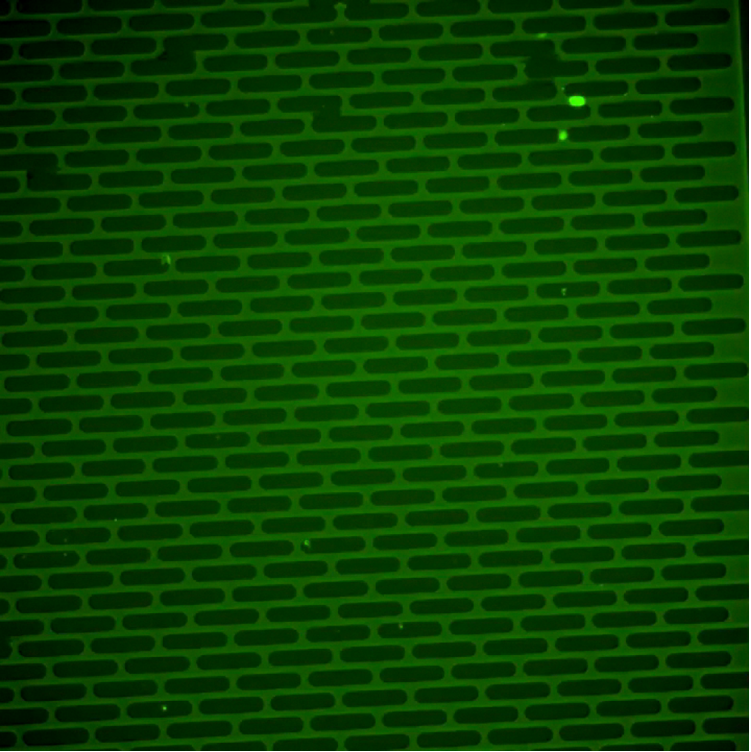
\includegraphics[width=\textwidth]{images/caspase_onset_sample}
  \caption{}
  \label{fig:caspase_onset_sample}
\end{subfigure}%
~
\begin{subfigure}{0.3\textwidth}
  \centering
  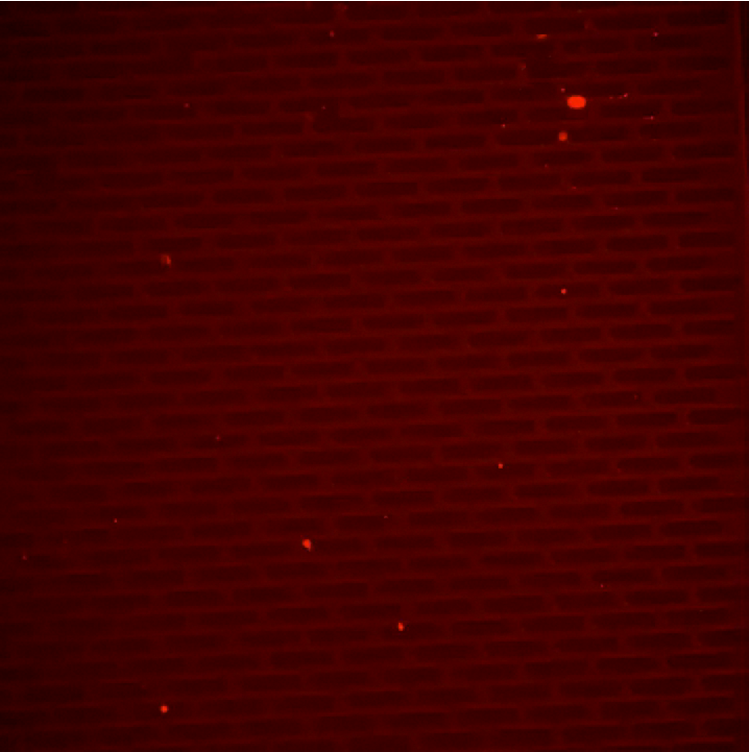
\includegraphics[width=\textwidth]{images/pi_onset_sample}
  \caption{}
  \label{fig:pi_onset_sample}
\end{subfigure}%

\caption[Example of images from green and red fluorescent channels]{Example of images captured in (a) green and (b) red fluorescent channels. Upon programmed cell death, the bright emission is detected in corresponding channels coming from the activation of PI and Caspase 3/7 expression paths.}

\label{fig:onset_samples}
\end{figure}

\subsection{Cell death determination}

Since each micro-trench is uniquely identified in this pipeline, assigning location of a cell tree with a micro-trench it is placed is the matter of finding which contour contains the starting coordinate of a cell track. We can thus combine the tracking information from both brightfield and fluorescent images to create cell death signal-corrected tracking data. Figure \ref{fig:cell_death_def} shows how it is done. First, we have one bright field cell track associated with one micro-trench. The next step would be to find out whether there is one fluorescent cell track associated with the micro-trench. Had there any, the death time of the cell is then updated to the start of fluorescent the cell track. However, since not every micro-trench is associated with one cell track (see Figure \ref{fig:microtrench_sample} for typical view of a well and Figure (TODO  Ch. 4) for the occupancy distribution of the micro-trenches), several considerations have to be made. Following is the table of possible occupancy scenario and what to do with the data (BF: brigtfield, FS: fluorescent) in unsynchronized experiment:

\begin{table}[H]
\centering
\begin{tabular}{ c | c | c | l  }
Trees\textsubscript{BF} & Children\textsubscript{BF} & Trees\textsubscript{FS} & Remark \\
\hline
0 & 0 & NA & Do nothing, not relevant for analysis\\
1 & 1 & NA & Do nothing, cell not dividing \\
1 & 2 & 0  & Do nothing, cell not dying \\
1 & 2 & 1  & Correct TTD; dead cell analyzed for TTD \\
1 & 2 & 2  & Correct TTDs; dead cells analyzed for TTD and SC \\
1 & 2+ & NA & Do nothing, some clones divided $> 1$ times\\
2+ & NA & NA  & Do nothing, too many cells \\
\end{tabular}
\caption[Scenario for time-to-death (TTD) and sister death time correlation (SC) analysis of unsynchronized experiment]{Scenario for time-to-death (TTD) and sister death time correlation (SC) analysis  of unsynchronized. Trees: number of cell tracks; Children: number of leaves. BF: brightfield; FS: fluorescent. Note that the cell tracks do not branch in FS.}
\label{table:scenario_unsynchronized}
\end{table}

The scenario for synchronized experiment is described in following table:

\begin{table}[H]
\centering
\begin{tabular}{ c | c | l  }
Trees\textsubscript{BF} & Trees\textsubscript{FS} & Remark \\
\hline
0 & NA & Do nothing, not relevant for analysis\\
1 & NA & Do nothing, cell not dividing \\
2 & 1 & Correct TTD; dead cell analyzed for TTD \\
2 & 2 & Correct TTDs; dead cells analyzed for TTD and SC \\
3+ & NA & Do nothing, too many cells \\
\end{tabular}
\caption[Scenario for time-to-death (TTD) and sister death time correlation (SC) analysis of unsynchronized experiment]{Scenario for TTD and SC analysis of synchronized experiment. Note that the number of cell track is equal to the number of leave in BF in synchronized experiment.}
\label{table:scenario_unsynchronized}
\end{table}

\begin{figure}[H]

\centering

\begin{subfigure}{\textwidth}
  \centering
  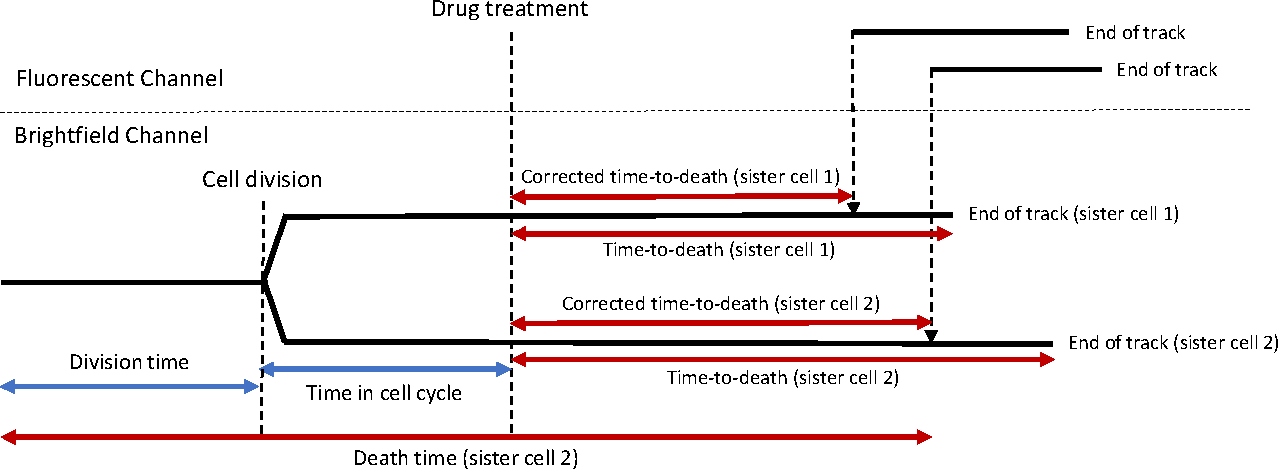
\includegraphics[width=\textwidth]{images/cell_death_def_unsyn.pdf}
  \caption{}
  \label{fig:cell_death_def_unsyn}
\end{subfigure}%

\begin{subfigure}{.75\textwidth}
  \centering
  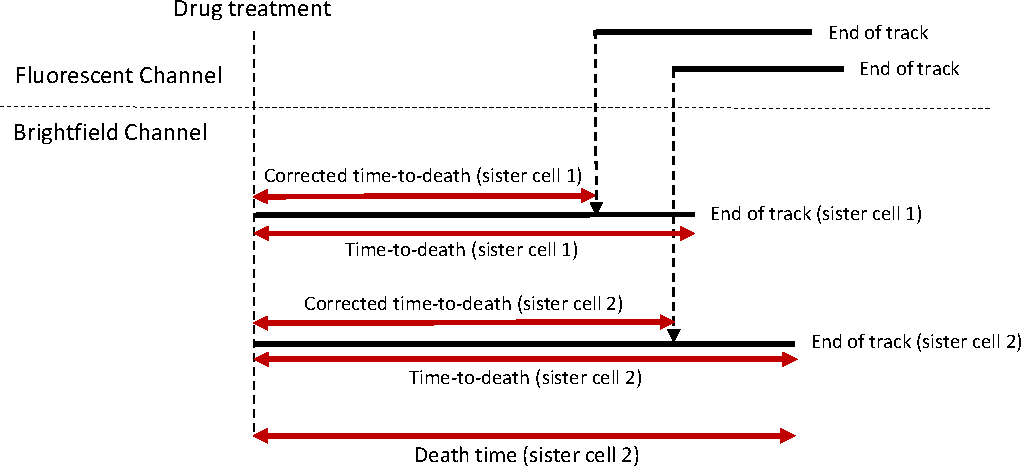
\includegraphics[width=\textwidth]{images/cell_death_def_syn_2.pdf}
  \caption{}
  \label{fig:cell_death_def_syn_2}
\end{subfigure}%

\caption[Definition of terms in time-to-death analysis and sister death correlation analysis]{Schematic overview of cell tracking in unsynchronized and synchronized experiments. (a) Various definitions used in unsynchronized experiment. (b) Various definitions used in synchronized experiments. Note that in case micro-trench with two tracks in fluorescent channel the assignment of the fluorescent to brightfield track does not affect time-to-death and sister-correlation analysis due to symmetric definition of time-to-death and time in cell cycle (i.e. the correlation of time-to-death between sister cells and time in cycle to time-to-death do not change no matter how the tracks assignment is done).}

\label{fig:cell_death_def}
\end{figure}

\begin{figure}[H]
\centering
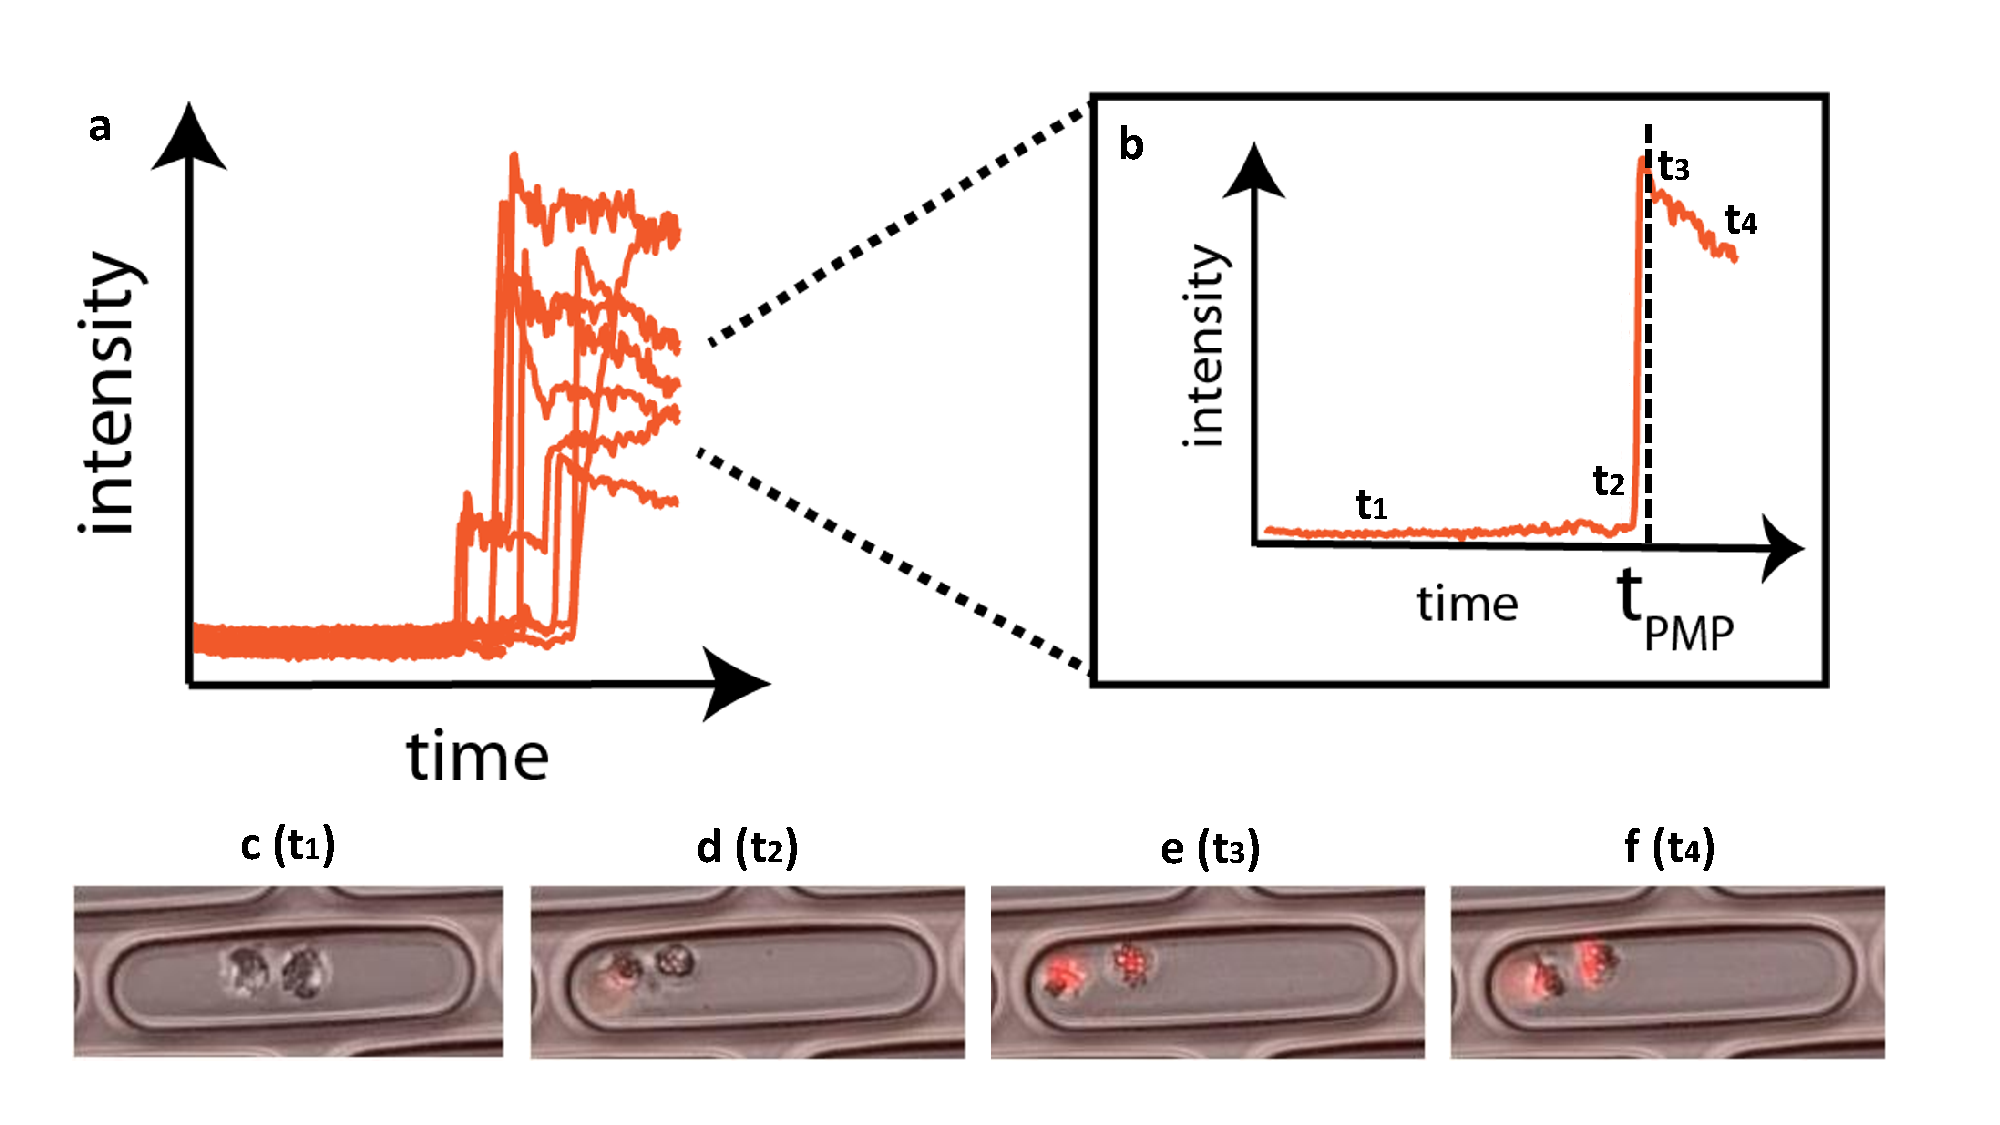
\includegraphics[width=\textwidth]{images/cell_death_detection}
\caption[Illustration of annotation of PI death signal]{Illustration of the annotation of of PI death signal emission as the cell death time ($t_{PMP}$). (a) How the total emission intensity will look like if it's being tracked (image taken for one related experiment of Radler's lab). (b) The hypothetical progression of total intensity of \textit{the cell on the left} upon treatment with some approximate time points representing various cell phases marked with $\mathbf{t_1}$, $\mathbf{t_2}$, $\mathbf{t_3}$ and $\mathbf{t_4}$. Initially, the left cell behaves normally upon treatment (c/$\mathbf{t_1}$). Only upon reaching the mitotic phase, the addition of Vincristine/Daunorubicin disrupts the process. Failure of entering the next phase sets the cell onto programmed cell death (d/$\mathbf{t_2}$). As the programmed cell death process advances, the PI emission became stronger (e/$\mathbf{t_3}$). At this point, the cel recognition will recognize the cell death signal as cell and thus represents cell death annotation. After a while, the emission will keep going on after a while (f/$\mathbf{t_3}$). We are, however, only interested with the onset time ($t_{PMP}$) to determine the cell death time and correct the track data (see Figure \ref{fig:cell_death_def}). Note especially the difference of onset time between the left and right cells. At $\mathbf{t_2}$, the left cell has begun programmed cell death process while the right cell has not. This difference in time-to-death between sisters is one of the focuses of the project.
}
\label{fig:cell_death_determination_example}
\end{figure}

%\section{Single cell tracking in the fluorescent channel (old)}

%Caspase and PI are imaged in the red (PI) and green (Caspase) fluorescent channel and used as indicator of cell death. Dying cells stop moving, become small and unstructured, and loose a distinctive bright signal in the brightfield channel, which makes them hard to track. We thus track dying cells in the fluorescent channels and concatenate the tracks with earlier tracks in the brightfield to determine time-to-death. To track cells in the fluorescent channel, we apply the following pipeline (see Figure \ref{fig:pipeline2}a):

%\begin{enumerate}
%\item We first adjust brightness and contrast manually (Figures \ref{fig:pipeline2}a and \ref{fig:pipeline2}b and Subsection \ref{subsubsection:brightness_contrast_adjustment}) in the similar fashion to the step taken to create micro-trench mask.
%\item The image then undergoes mean correction of static noises by subtracting each image with average intensity over all imagess (Figures \ref{fig:pipeline2}c and \ref{fig:pipeline2}d and Subsection \ref{subsection:substraction_by_mean}).
%\item Subsequently, the detection and tracking part of image computing pipeline is identical to brightfield images' (Figure \ref{fig:pipeline1} and Subsections \ref{subsection:cell_recognition} and \ref{subsection:cell_tracking})
%\item Eventually, death time of a cell is indicated by the onset of fluorescence track being recognized in red or green channel, depending on treatment:or Vincristine treatment and control, the cell death is based on tracks in red (PI) channel while the cell death in Daunorubicin treatment is based on green (Caspase) channel (Subsection \ref{subsection:cell_death_signal_determination}).
%\subsection{Cell death signal determination}
%\label{subsection:cell_death_signal_determination}

\section{Pipeline visualization}

The image processing pipelines for both brightfield and florescence channels can be seen in following figures:

%TODO separate huge images into smaller images
%TODO add following explanation:
%Brightfield channel pipeline. (j) The original out-of-focus image of the upper left corner of  the image position 41. (k) The view of the same area as (l) after applying brightness and contrast adustment. (m) The view of the same area after applying RATS on image in (n) showing the contour of micro-trenches in the area. (d) The contours filled with neutral color (black). Note that some micro-trenches are not filled as they are open and thus topologically not the outernmost contours. Scale bar on the uppermost figure is $100 \mu M$ long

\begin{landscape}
\begin{figure}[H]
   \centering
    %\includegraphics[width=1.0\textwidth]{Image.eps}
    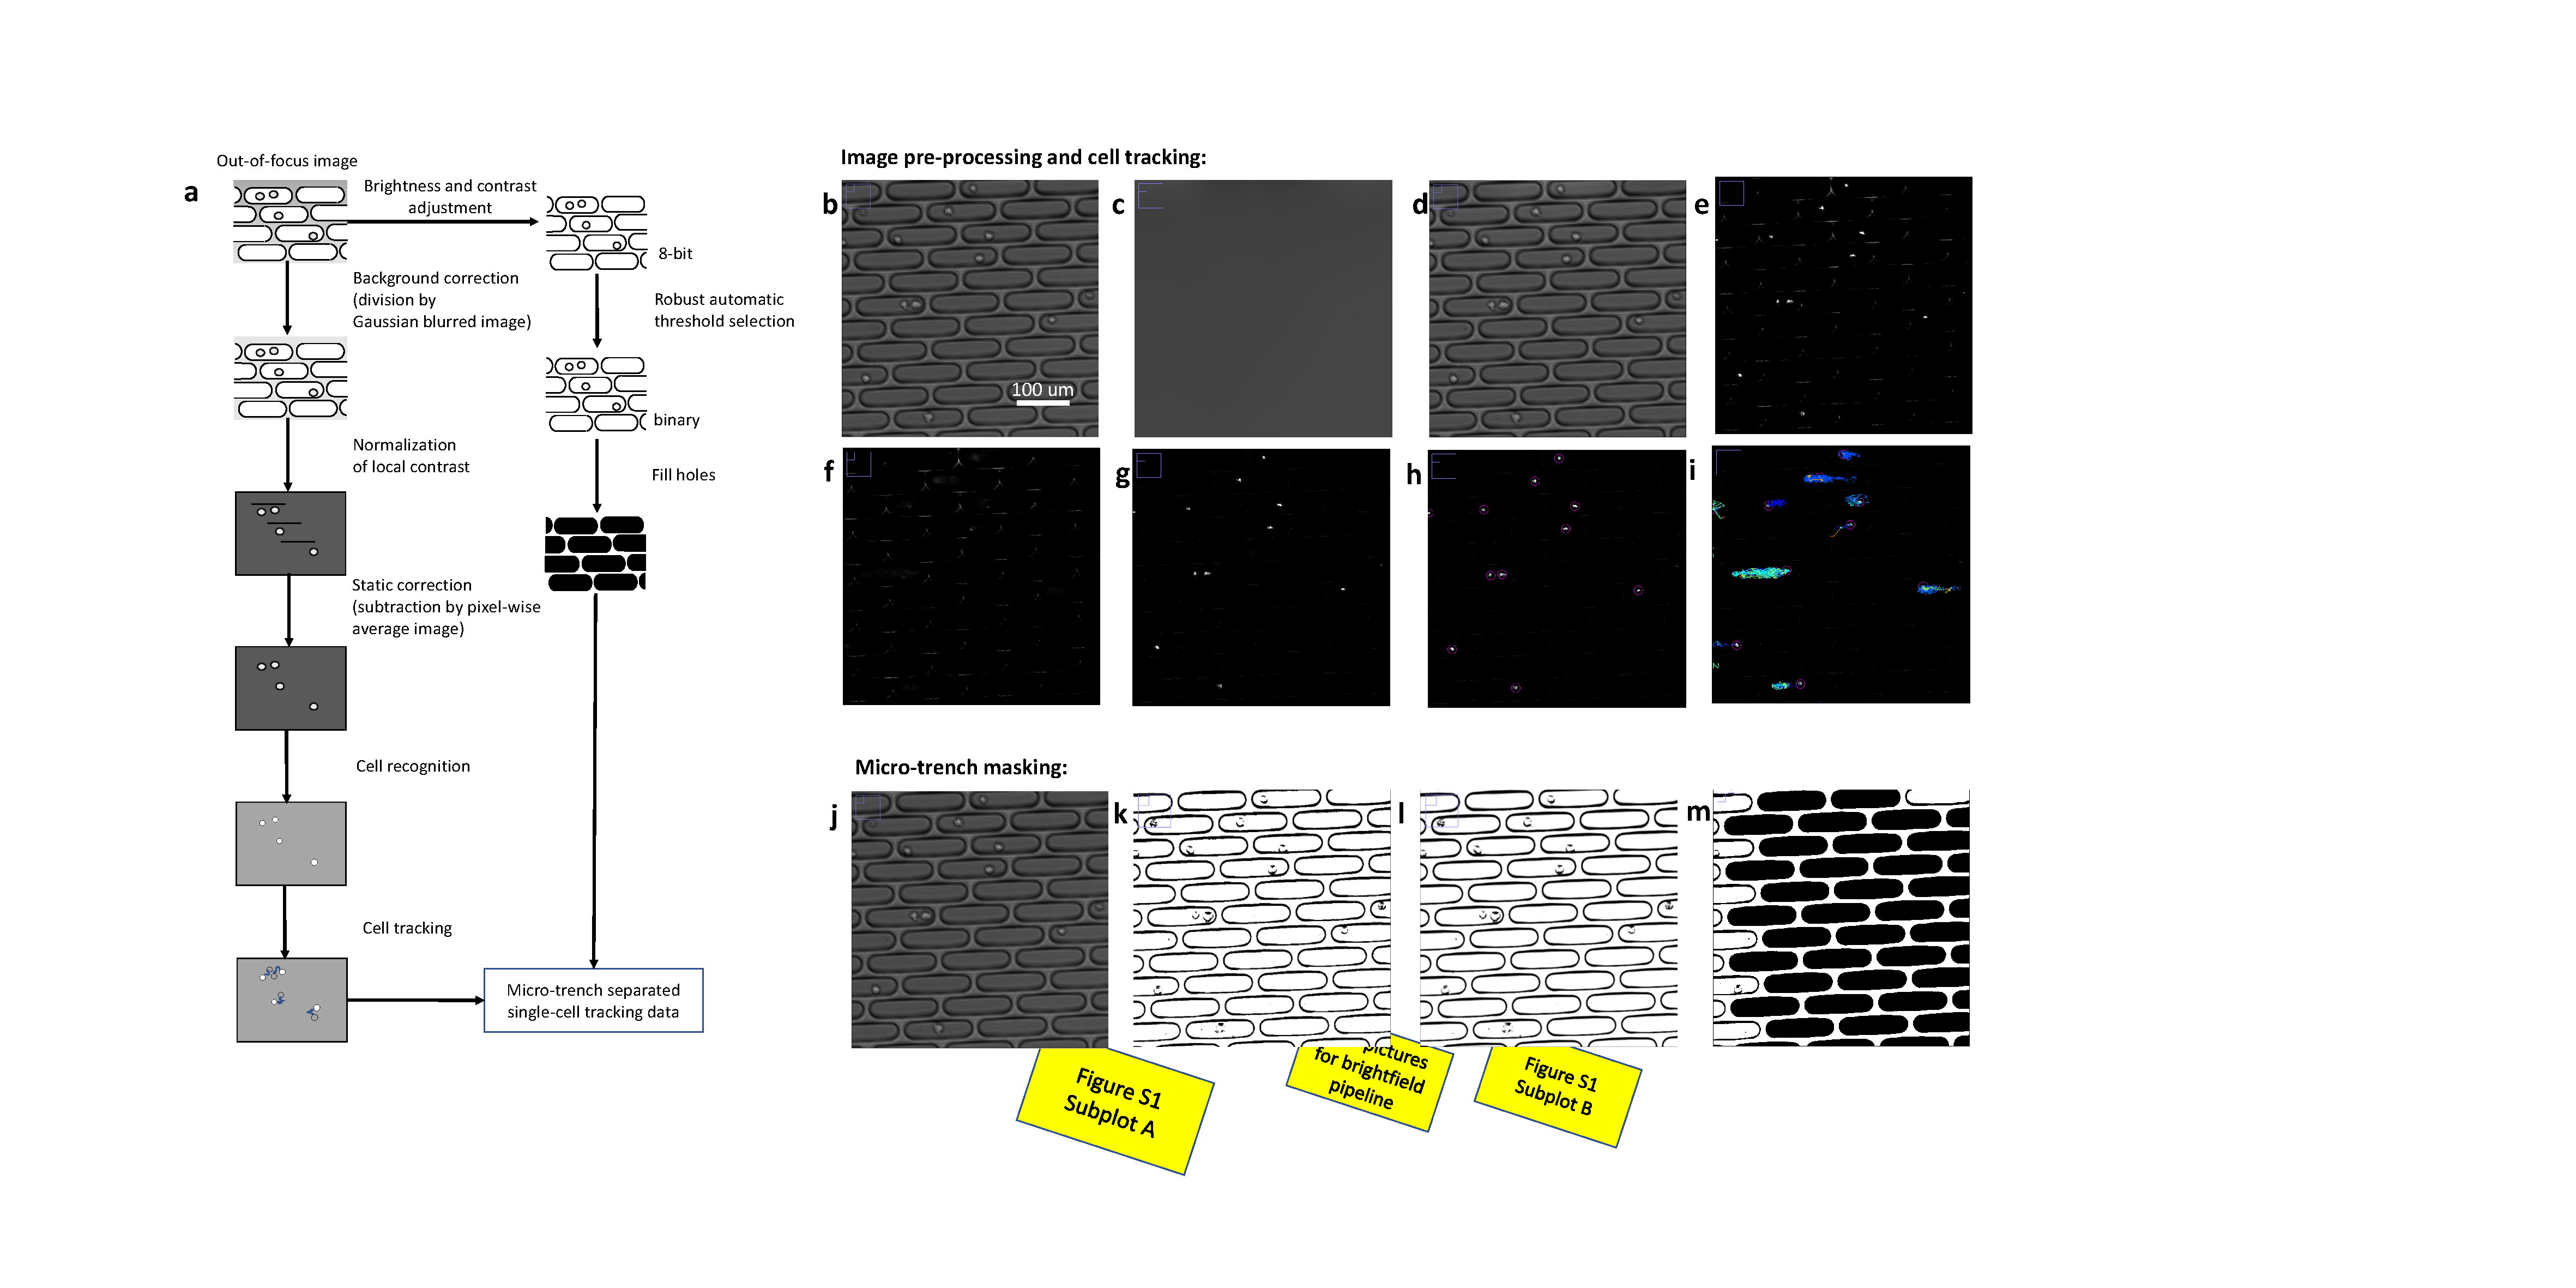
\includegraphics[height=0.95\textheight]{images/pipeline/01.pdf}
    \caption[Brightfield channel pipeline]{}
\end{figure}
\label{fig:pipeline1}
\end{landscape}

\begin{landscape}
\begin{figure}[H]
   \centering
    %\includegraphics[width=0.5\textwidth]{Image.eps}
    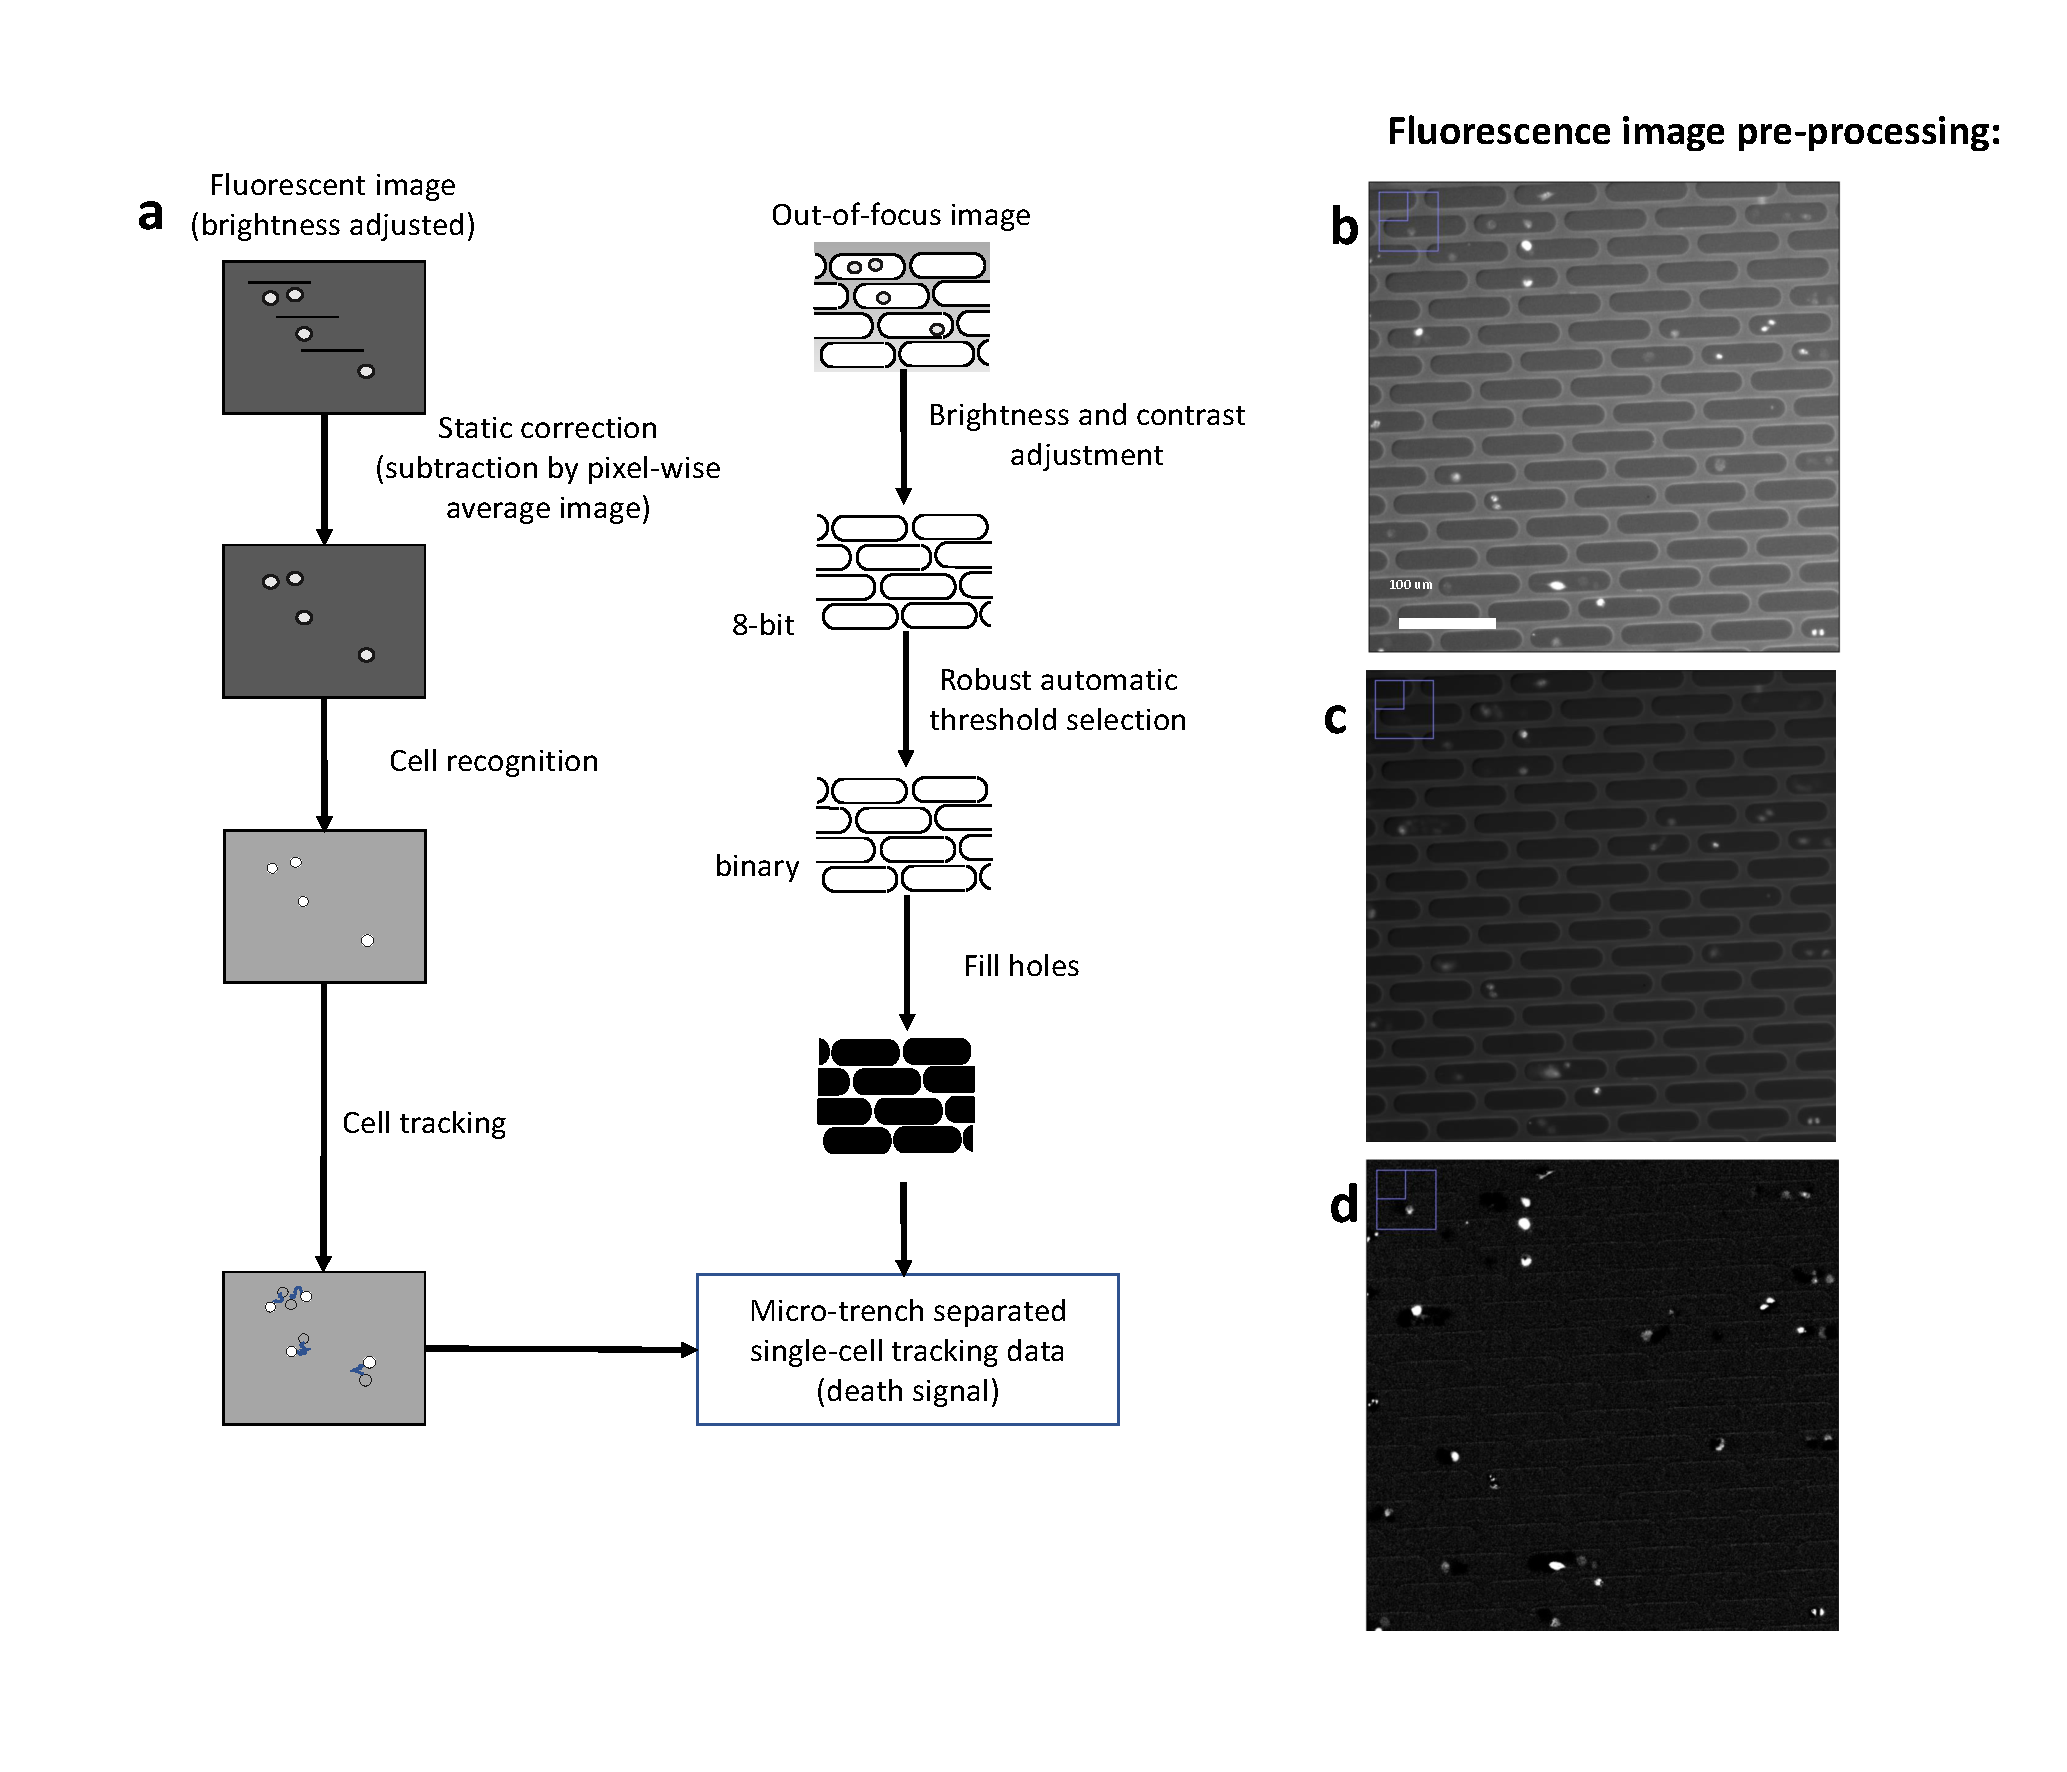
\includegraphics[height=\textheight]{images/pipeline/02.pdf}
    \caption[Fluoroscence channel pipeline]{Fluoroscence channel pipeline}
\end{figure}
\label{fig:pipeline2}
\end{landscape}

\begin{figure}[H]
   \centering
    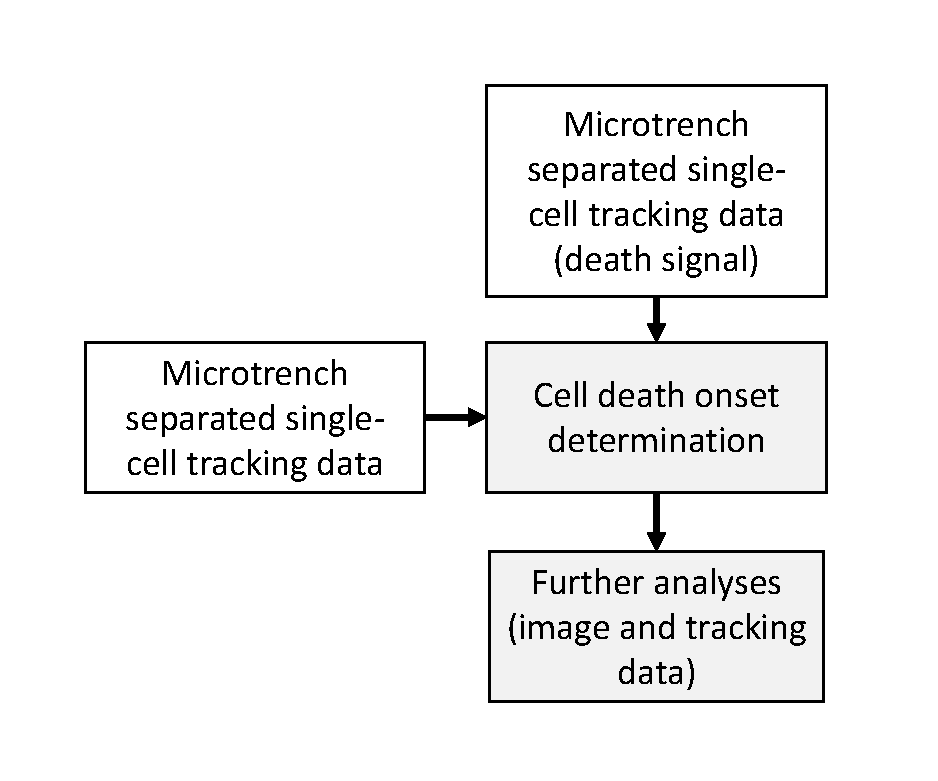
\includegraphics[height=0.5\textwidth]{images/pipeline/03.pdf}
    \caption[Combination of tracking data with cell death information creating cell death signal-corrected tracks data]{Combination of tracking data with cell death information creating cell death signal-corrected tracks data.}
    \label{fig:pipeline3}
\end{figure}

\section{Implementation and availability}

The image and tracking data is combined and post-processed using Python scripts utilizing OpenCV\cite{bradski2008learning}, NumPy \cite{walt2011numpy}, pandas \cite{mckinney2010data} and Matplotlib \cite{hunter2007matplotlib}, and the Jython and Trackmate \cite{tinevez2017trackmate, pedroni2002jython} plugin in Fiji \cite{schindelin2012fiji}. The Python package scikit-learn is used for training and testing both support vector machine and random forest \cite{scikit-learn}. Our code is available at:

\href{https://github.com/raharjaliu/MA/tree/master/source}{https://github.com/raharjaliu/MA/tree/master/source}.

\chapter{Results}

%TODO adjust and add

In this chapter the findings of the project are presented. The application of the pipeline in the image yields actionable data which in turn are analyzed. The chapter is separated into various parts:

\begin{itemize}
\item Distribution of cell cycle duration times. Here we analyze how the cell cycle duration time varies by cells in the wells.
\item Variability of time-to-death between sister cells.
\item Variability of time-to-death by time-in-cycle.
\item Machine learning models of cell death.
\end{itemize}

\section{Occupancy of micro-trench}

\section{Distribution of cell cycle duration times}

Daughter cells contained in the micro-trenches and being separately trackable (Figure 2a) allow to accurately determine the cell cycle length (Figure 2b) and the time difference in division time points between sister cells (Figure 2c). For each cell, we determine the first division time point t0, the second division of the first daughter cell at time t1, and the division second daughter cell at t2. Figure 2a also shows an exemplary image series of one trench filled with initially one cell which gives rise to four cells within the first 30 hours. In our experiments 320 MOLM-13 cells were observed for 40 hours to detect a minimum of two divisions. The cell cycle duration distribution with a mean of $19.7 \pm 2.6$ (mean $\pm$ std) hours is well described by both a lognormal distribution (red dotted line, Figure 2b) and a gamma distribution (dashed blue line, Figure 2b). Figure 2c shows the distribution of the difference between the cell cycle duration times for sister cells. In this case, 160 pairs of daughter cells were analyzed. The dashed blue line is a gamma distribution fit with a mean value of 2 h. In the inset a correlation plot of the cell cycle duration times for sister cells (black dots) and for randomly paired cells (red dots) is presented. Daughter cells divide in a highly correlated manner with a Pearson correlation of r=0.85, while random paired cells show a much smaller correlation (r=0.25).

The observed lognormal cell cycle duration distribution is well documented in literature, with both the size of mammalian cells as well as cell doubling times following a lognormal distribution [26, 27]. The underlying mechanism of cell division timing is an active field of research. It is however assumed that the so-called added model accepted in bacteria [28] is also valid in somatic cells. In general size regulation can arise from various types of coupling between cell size, cell growth and cell cycle progression [29]. It has also been proposed, based on a coupled mathematical model of mammalian cell cycle and circadian clock, that the circadian clock triggers critical size control in the mammalian cell cycle and that it is more readily observed in cell lines that contain circadian rhythms [30]. In this context it is important that the adder mechanism also predicts exponential time correlation between sister cells as observed in our experiments [28]. 


\section{Variability of time-to-death between sister cells}

\section{Variability of time-to-death by time-in-cycle}

MOLM-13 cells were seeded from the cell culture flask in the micro-trenches array and directly placed under the time-lapse microscope. Mother cell mitosis, i.e. the division time (t0), is used as a reference point of the cell-phase indication. After 20 hours, when most cells had divided once based on the previously measured cell cycle duration distribution (Figure 2b), the drugs (Vincristine or Daunorubicin) were added (Figure 3a). Time-lapse movies were simultaneously taken in brightfield and fluorescence. To track the cells in an automated routine (see Methods) we acquired the brightfield images in a slightly defocused mode (focus at -20 μm), which resulted in images with slightly blurred but well peaked intensity distribution. Fluorescence images of both the propidium iodide (PI) and the Cell Event Caspase 3/7 marker for the Vincristine data and of only the Cell Event Caspase 3/7 marker for the Daunorubicin data, since Daunorubicin is autofluorescent in the red region, were acquired. In Figure 3a a timeline of the experimental procedure is shown together with exemplary brightfield and fluorescence (PI marker) images are shown in overlay.

The measured time-to-death distribution is shown in figures in 3b for increasing drug concentration. The red black curves represent the Kernel density estimation of the probability density function of each histogram. The plots in Figure 3c depict, for each drug treatment, a scatter plot of the time passed in the cell cycle, i.e. the time passed from the division until the drug was added, with the time-to-death i.e. the time passed from the drug administration time point until the death of the cell. The blue lines are best linear fits and show the dependence of the time-to-death on the time spent in the cell cycle. The colored areas indicate the cell cycle phase based on the division distribution in figure 2b, the duration for each phase is calculated based on the phase durations proposed in T. S. Weber et al. 2014 [32]. We observed a negative correlation between the time in the cell cycle and the death time, which increased for increasing VCR concentrations (1-100 nM), but there was no correlation for the highest VCR concentration (1000 nM), indicating that in this high concentration side effect toxicities are prominent. The Pearson product-moment correlation test results are presented in Table 1. In the case of Daunorubicin (100 nM), we observed an even stronger negative correlation between the time spent in the cell-cycle and the time-to-death in the case of Daunorubicin (100 nM). Especially the time-to-death of the cells that were in the S phase when the drug was added, the phase in which Daunorubicin should be more effective, had a larger deviation in comparison to the time-of-death of cells that were in the G1 or in the G2/M phase. 

Comparison of synchronized and unsynchronized populations. We performed a cytotoxic test on the micro-trenches array using a synchronized cell population with the "double thymidine block" procedure [33] (Figure 4). Thymidine arrests cells at the G1/S border, which is after the division time point within the length of G1 phase. Cells were released 3 h before the start of imaging and seeded in micro-trenches. The drug was added just before starting imaging. In Figure 4a, we show a timeline of the experimental procedure. In Figure 4b, we plot the distributions of the time-to-death in each drug concentration. The blue black curves represent the Kernel density estimation of the probability density function of each histogram. For all drug concentrations the maximum of these distributions is near the 15th hour after starting imaging.

In Figure 5 we compare our results of the unsynchronized cell population (Figure 3) with a cell population synchronized with thymidine block (Figure 4). For both the unsynchronized and the synchronized population, the total number of dead cells as a function of drug concentration is shown in Figure 5a and shows the expected increase in death response with increasing dose. Figure 5b, shows the death times between the synchronized (blue) and the unsynchronized (red) population. The distributions plotted are the normalized number of cells in all drug treatments, for all cells tracked. Apart from a peak at the beginning of the measurement in the synchronized population, the shape of the two distributions is equivalent. In the synchronized population less cells haves a short time-to-death, especially evident in the VCR 1000 nM concentration (Figure 3b and 4b), indicating that the synchronized population is more resistant to death. In Figure 5c, we show scatter plots of the time-to-death between sister cells in an ensemble of all drug treatments. The Pearson correlation coefficient (r) is 0.5 (medium correlation) for the sister cells of the unsynchronized population and 0.06 for the synchronized. The ellipses indicate the directionality of the correlation. Thus, the time-to-death between sister cells was positively correlated for the unsynchronized population but not for the synchronized.


\section{Machine learning models of cell death}
\label{section:ml_results}

\chapter{Summary and Outlook}

We showed that arrays of micro-structured trenches provide a platform that enables a label-free method for tracking cells and for approximating the cell cycle phase without the use of molecular markers. Our approach allows to set individual clocks in single cells using the first division for each occupied trench as a starting point. This is highly accurate and overcomes typical drawbacks of low detection efficiency of fluorescence-based indicators such as the FUCCI marker, which usually have low transfection efficiency round 20-40\%, and generally short duration of staining, namely ~15 hours, which is no sufficient for our long-time measurements. By compartmentalizing the cell population in small groups we enable an image-based cell tracking. Without the use of such an array, time-lapse observation of a cell population for such long hours, even beyond 48 hours, is impossible for both adherent and non-adherent cells since cells escape from the field of view very fast, within a few hours. In addition, compartmentalization of the cell population not only reduces the error of mixing the identities of adjacent cells but also the time and computational power needed for tracking.

In addition, we demonstrate the practicability of the micro-trench platform to determine the time-to-death after induction of cell death with vincristine and daunorubicin. At high concentration vincristine stimulates microtubule depolymerization and mitotic spindle destruction. At lower clinically relevant concentrations, it blocks mitotic progression. As a result, we expected a negative correlation between the time spent in the cell-cycle and the time-to-death in the case of VCR, since a cell that spent a long large amount of time in the cell-cycle should be closer to the M-phase so it should have a shorter time-to-death i.e. it should die earlier. Indeed here we observed that the time-to-death negatively correlates with the time spent in the cell cycle and that this correlation becomes more prominent with increasing VCR concentration up to 100 nM, but there is no correlation at the highest concentration (1000 nM). The reason for no correlation in the 1000 nM might be side effect toxicities that happen through the whole cell cycle and as it has been shown before [12], after exposure to antimitotic drugs cells display complex fate profiles, such as unequal cell division producing aneuploid daughter cells, exiting the cell cycle without undergoing cell division (mitotic slippage), or exiting G1 and undergoing apoptosis or senescence. On the other hand, the correlation of the time-to-death with the time spent in the cell cycle is more prominent in the case of Daunorubicin (100 nM) and the deviation of the time-to-death for the cells in the S-phase during drug addition, is larger compared to the cells in G1 or G2/M phase (Figure 3b).

We furthermore find that the sister cell correlations of the time-to-death for the unsynchronized and the synchronized populations differ. We observed similar response between sister cells in the unsynchronized experiment as far as the time-to-death is concerned, during an observation period of 24 hours after the addition of the drugs. At the same time the distributions of the time-to-death (average of all different drug concentrations) of the unsynchronized and the synchronized populations are similar, which would suggest that synchronizing the cells with the double thymidine block did not affect their response to both tested drugs. However, a closer look into the data and especially when analyzing the response between sister cells of the synchronized population, we observed that there is no correlation of the time-to-death between sister cells, contrary to the results from the unsynchronized population. This observation suggests that the double thymidine block procedure has an effect on sister cell response heterogeneity to vincristine and daunorubicin. Sister cell response variability is a matter drawing attention since it is an indication whether different phenotypes stems from genetic differences or from differences in the protein state of the cells. The results available so far strongly depend on the cell process that is interrogated. For instance, it has been previously reported that sister cells undergo apoptosis synchronously [5, 34]. However, in response to antimitotic drugs the fate of one sister is independent of the fate of the other [12]. In another study, sister cell fate in response to TRAIL-induced apoptosis correlated, as did also the time-to-death between HeLa sister cells but this correlation decayed as a function of time since division, the time period tested was 8 hours. Based on this observation, the transient heritability in fate model was proposed, which states that protein synthesis promotes cell divergence so that sister cells soon become no more similar to each other than random paired cells[1].

In future work, the micro-trenches array can be used with more than one drug, namely for combination therapy, to determine the optimal administration timing of each drug. Microfluidic devices have facilitated single-cell studies and boosted the collection of quantitative experimental data, such as the measurement of single-cell mass with high accuracy[35]. Measuring the cell size or the volume added to the cell after its mother division are crucial quantitative data to elucidate the underlying mechanisms that drive cell division. The micro-trenches array coupled with time-lapse microscopy and automated image analysis is a step toward this direction.

%TODO complete

\section{Fully automated microfluidics pipeline}

\section{Fully automated pipeline for single-cell analysis}


Improvements in analysis pipeline:

\begin{itemize}
\item better method for masking recognition
\item possibly even machine learning based methods
\end{itemize}

\begin{verbatim}
I. Summary (and discussion?)
Connect Results with Background

II. Outlook
Improvemnt capability
\end{verbatim}

\subsection{Automated micro-trench masking}

One positive thing about the design of our data analysis pipeline is the modularity of its component. As mentioned multiple times in this thesis (in particular in Subsection \ref{subsection:micro_trench_masking}, our method can well be improved by automatizing the micro-trench masking process. Although itself not a bottleneck of the process, as the entire dataset of 63 image positions could be processed in less than an hour, automating this process will save time and more importantly, clicking and draging efforts, thus lets scientists do the things that matter more for them.

There are several methods that came to mind in improving the micro-trench masking, which generally can be separated in two groups: ML-based methods and non-ML-based methods. ML-based methods generally require either a manual annotation of correctly recognized micro-trench (a class of methods called supervised learning methods) or certain prior knowledge regarding distinctive features of micro-trench that separate it from background image and/or the cells (a class of methods called unsupervised/semi-supervised learning methods).

In the following part of this subsection various potential implementations of both ML-based and non-ML-based methods are listed down.

\subsubsection*{Maximally interesting extremal region (MNER)}

Introduced by Oliver Hilsenbeck in his master's thesis in 2014 \cite{hilsenbeck2014maximally} %TODO continue


%TODO

%% BIBLIOGRAPHY %%

\bibliographystyle{unsrt}
\bibliography{mabib}

%% APPENDICES %%

\begin{appendices}
\newpage

\chapter{Tables}
\label{chapter:appendix_tables}

\section{Inferred shift in wells}

\begin{table}[H]
\centering
\begin{tabular}[t]{ c | c | c }
Position & $\delta_x$ & $\delta_y$
\\
\hline
01 & -2 & -4
\\
02 & -3 & -4
\\
03 & -3 & -4
\\
04 & -3 & -4
\\
05 & -3 & -3
\\
06 & -3 & -4
\\
07 & -3 & -4
\\
08 & -4 & -3
\\
09 & -4 & -4
\\
10 & -4 & -4
\\
11 & -4 & -4
\\
12 & -4 & -3
\\
13 & -4 & -3
\\
14 & -5 & -3
\\
15 & -5 & -3
\\
16 & -6 & -5
\\
17 & -6 & -5
\\
18 & -6 & -5
\\
19 & -6 & -5
\\
20 & -6 & -4
\\
21 & -7 & -5
\end{tabular}
~
\begin{tabular}[t]{ c | c | c }
Position & $\delta_x$ & $\delta_y$
\\
\hline
22 & -7 & -4
\\
23 & -7 & -4
\\
24 & -9 & -4
\\
25 & -9 & -5
\\
26 & -8 & -5
\\
27 & -8 & -4
\\
28 & -8 & -4
\\
29 & -8 & -4
\\
30 & -8 & -4
\\
31 & -8 & -4
\\
32 & -8 & -3
\\
33 & -9 & -3
\\
34 & -8 & -3
\\
35 & -8 & -3
\\
36 & -9 & -2
\\
37 & -9 & -3
\\
38 & -9 & -2
\\
39 & -8 & -2
\\
40 & -7 & -3
\\
41 & -7 & -3
\\
42 & -7 & -3
\end{tabular}
~
\begin{tabular}[t]{ c | c | c }
%\hline
Position & $\delta_x$ & $\delta_y$
\\
\hline
43 & -7 & -3
\\
44 & -7 & -3
\\
45 & -7 & -3
\\
46 & -7 & -3
\\
47 & -7 & -2
\\
48 & -4 & -2
\\
49 & -4 & -2
\\
50 & -4 & -2
\\
51 & -4 & -2
\\
52 & -4 & -2
\\
53 & -5 & -2
\\
54 & -5 & -2
\\
55 & -4 & -1
\\
56 & -2 & -2
\\
57 & -3 & -3
\\
58 & -3 & -3
\\
59 & -3 & -2
\\
60 & -3 & -2
\\
61 & -3 & -3
\\
62 & -3 & -2
\\
63 & -4 & -2
\end{tabular}
\caption{The inferred shift (in pixels) for each image position in unsynchronized experiment. The shifts are inferred using the shift correction algorithm explained in Subsection \ref{subsection:shift_correction}.}
\label{table:inferred_shift}
\end{table}


\chapter{Experiment Protocols}

%\section{Micro-trenches array fabrication}
%\label{appendix:microtrench}

%\subsection*{Photolithography of the SU-8 wafer}

%The fabrication of the SU-8 (MicroChem Corp, USA) wafer was executed in a in-house cleanroom facility using a ProtoLaser LDI system (LPKF Laser \& Electronika, Naklo, Slovenia), with a 375 nm wavelength laser and 1 μm spot diameter.

%\subsection*{Softlithography and micromolding}

%Polydimethylsiloxane (PDMS) prepolymer solution is mixed with the crosslinker in a 10:1 ratio (w/w) (Sylgard 184, Dow Corning, USA) and then degassed under vacuum. PDMS is then purred on the SU-8 wafer, degassed and cured in 50 oC. The resulting PDMS stamp is peeled off the wafer and cut into appropriate shapes. The PDMS pieces, with 25 1/4 pillars in height, are activated with argon plasma and then immediately placed upside down on a silanized with TMSPMA (3-(Trimethoxysilyl)propyl methacrylate, Sigma-Aldrich) glass coverslip. A solution of PEG-DA (Mn=258) containing 2\% v/v of the 2-hydroxy-2methylpropiophenone (both from Sigma-Aldrich, Germany) is freshly prepared and then a drop is deposited at the edge of the PDMS stamp. The PDMS stamp is filled by capillary force induced flow. PEG-DA is then polymerized in an UV-ozone cleaning system (UVOH 150 LAB, FHR, Ottendorf, Germany). Next, the PDMS stamps are peeled off and the resulting micro-trenches of cross-linked PEG-DA are dried in an oven (Binder GmbH, Tuttlingen, Germany) overnight at 50oC. Finally, the slides are sonicated with 70\% ethanol and distilled water before a sticky slide is attached on top (8-well sticky slide, ibidi GmbH, Munich, Germany).

\section{Images acquisition}
\label{appendix:imageacquisition}

%Imaging was performed under an inverted Nikon Ti Eclipse microscope with a motorized stage (Tango XY Stage Controller, M\"arzh\"auser Wetzlar GmbH \& Co. KG, Germany), a CFI Plan Fluor DL 10X objective, a pco.edge 4.2 Camera (PCO AG, Kelheim, Germany) and a Lumencor Sprectra LED fluorescence lamp. For detection of the Caspase-3/7 and the PI marker, the following filters were used respectively, 474/27 nm, 554/23 (excitation) and 515/35 nm, 595/35 nm (emission). Brightfield out of focus (-20 $\mu$m) images were taken every 10 minutes and in-focus  brightfield and fluorescence images every 30 minutes for 48 hours. Vincristine or Daunorubicin were added after 20 hours from the beginning of the imaging. During the recording samples were kept at a constant temperature of 37\degree C and CO2 using an Okolab heating and CO\textsubscript{2} 2 box (OKOLAB S.R.L., NA, Italy). For the synchronized population, the double thymidine block protocol was followed. Briefly, MOLM-13s cells at the exponentially growing phase were incubated in blocking medium (culture medium supplemented with 2 mM Thymidine (CAS 50-89-5, Calbiochem\textsuperscript{\textregistered}, Germany)) for 24 hours. Cells were then released and incubated in culture medium for 8 hours and finally were incubated in blocking medium for 12 hours. After 2 hours, the synchronized population was seeded in the slide bearing the micro-trenches together with the markers and drugs at the same conditions as the unsynchronized population, and imaged for 24 hours.

\section{Placeholder}

\end{appendices}

\end{document}